Compared to the previous chapter, where we worked in the thermodynamic limit, we now restrict the spin chain to a finite size $N$. Moreover, we explicitly break translation invariance by imposing open boundary conditions and allowing the tensors to be site dependent: 
\begin{equation}
	A^{[n]} \in \mathbb{C}^{D_{n-1} \times d \times D_n} \text{ with } D_0 = D_N = 1. 
\end{equation}
For computational basis indices $s_1, \ldots, s_N$, the finite matrix product $A^{[1] s_1} \cdots A^{[N] s_N}$ defines the probability amplitude of the $d^N$ dimensional \textit{matrix product state} (MPS)
\begin{equation} \label{eq:mps}
	\ket{\psi ( A^{[1]}, \ldots, A^{[N]} )} = \sum_{\{s_n\}} A^{[1] s_1} A^{[2] s_2} \cdots A^{[N] s_N} \ket{s_1 \ldots s_N} 
	= \raisebox{-0.57\height}{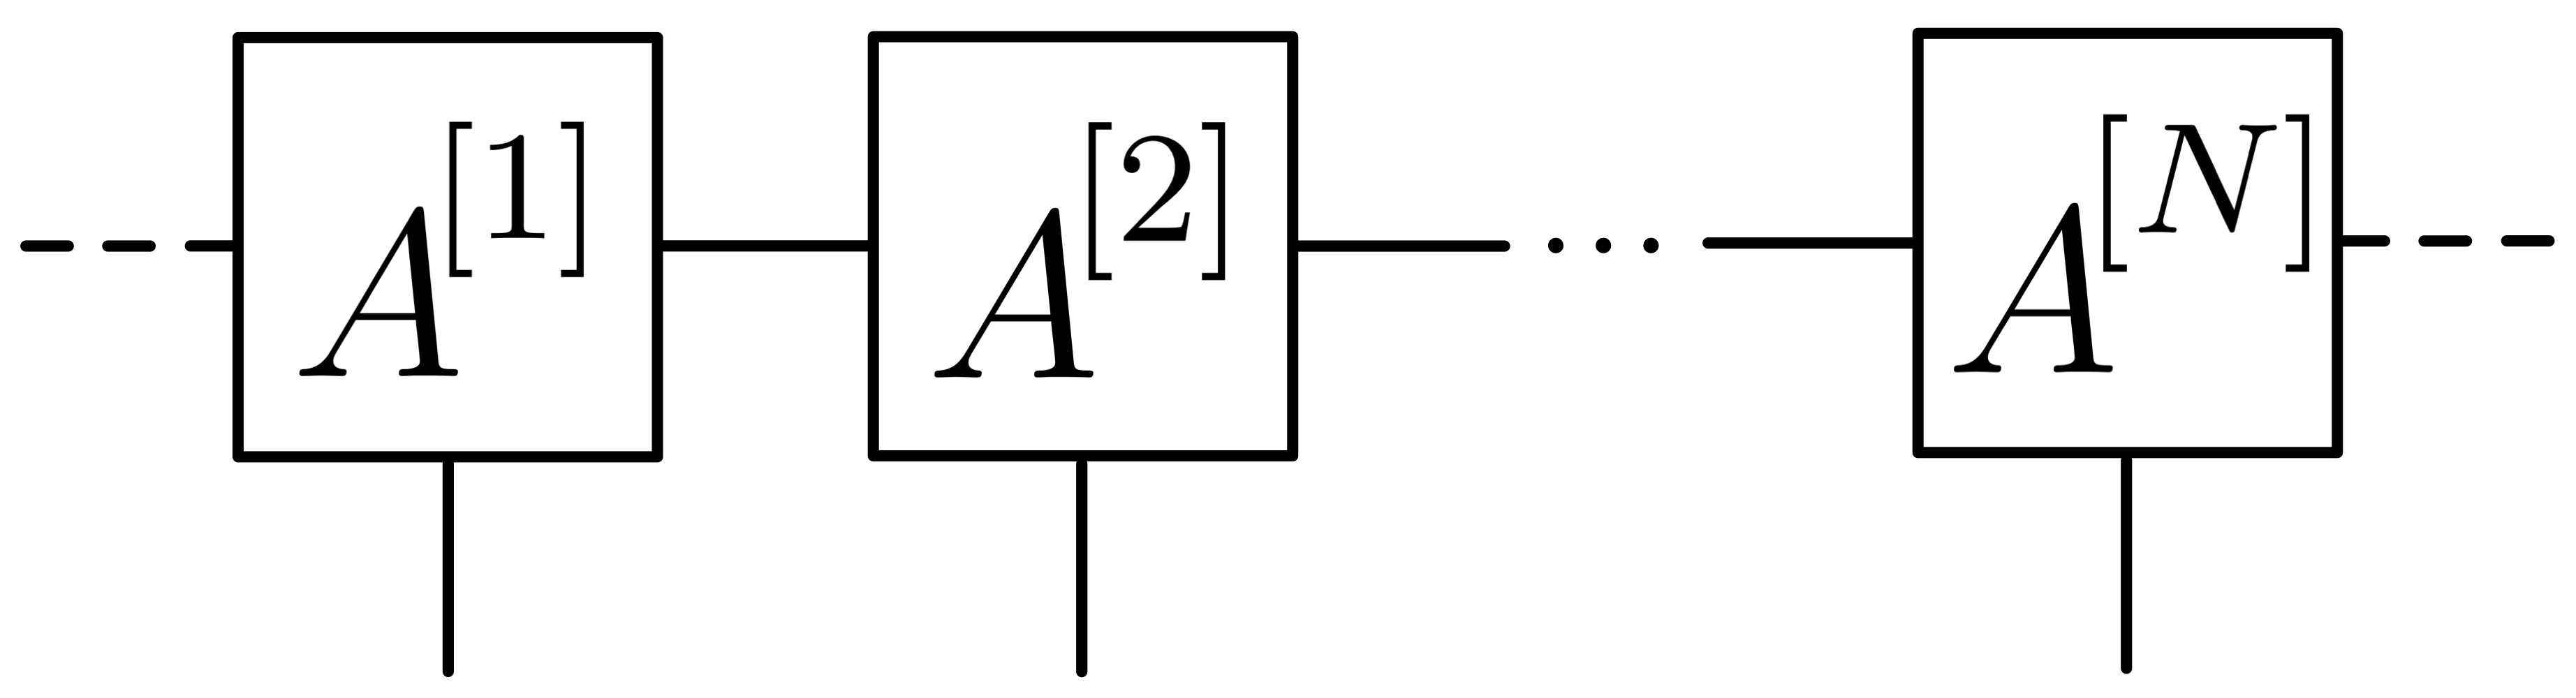
\includegraphics[height=1.3cm]{mps.png}} \hspace{0.2em} .
\end{equation}
Analogous to uMPS, for a fixed set of bond dimensions $\{ D_n \}_{n=1}^{N-1}$, we can define a complex manifold of tensors that is biholomorphic to the manifold of corresponding MPS. This was rigorously established in \cite{haegeman2014geometry}. The necessary restriction (in analogy to primitivity for uMPS) is now to tensors with positive definite \textit{virtual density matrices}. They are defined recursively via
\begin{align}
\begin{split} \label{eq:virtual_density_matrices}
	& l^{[0]} = 1, \hspace{0.5em} l^{[n]} = \sum_{s_n} {(A^{[n]s_n})}^{\dagger} l^{[n-1]} A^{[n]s_n},\\
	& r^{[N]} = 1, \hspace{0.5em} r^{[n-1]} = \sum_{s_n} A^{[n]s_n} r^{[n]} {(A^{[n]s_n})}^{\dagger},
\end{split}
\end{align}
for $n = 1, \ldots, N$. The gauge group is now the product $\prod_{n=1}^{N} \text{GL}(D_n, \mathbb{C})$ with the following transformation leaving the MPS invariant:
\begin{equation}
	B^{[n] s_n} = {(S^{[n-1]})}^{-1} A^{[n] s_n} S^{[n]} \text{ with } S^{[0]} = S^{[N]} \in \mathbb{C}.
\end{equation}
The group elements $\{ \{\alpha \mathbbm{1}_{D_n}\}_{n=1}^N \vert \alpha \in \mathbb{C}\}$ act trivially on the tensors $\{ A^{[n]}\}$ and therefore we have to quotient out $\text{GL}(1, \mathbb{C})$. Since the gauge group is a direct product containing $\text{GL}(D_N, \mathbb{C})$ with $D_N = 1$, we end up with $\prod_{n=1}^{N-1} \text{GL}(D_n, \mathbb{C})$ as the effective gauge group of the MPS manifold. In summary,
\begin{equation}
	\mathcal{A}_{\{D_n\}} = \left\{ \bigoplus_{n=1}^N \mathbb{C}^{D_{n-1} \times d \times D_n} \:\middle\vert\: l^{[n]}, r^{[n]} > 0 \text{ for all } n \right\} \Big / \prod_{n=1}^{N-1} \text{GL}(D_n, \mathbb{C})
\end{equation}
is biholomorphic to
\begin{equation}
	\mathcal{M}_{\{D_n\}} = \left\{ \ket{\psi ( A^{[1]}, \ldots, A^{[N]} )} \in \mathbb{C}^{d^N} \middle\vert \{ A^{[n]}\} \in \mathcal{A}_{\{D_n\}}\right\}.
\end{equation}
In section \ref{sec:dmrg} we will variationally approximate ground states within $\mathcal{M}_{\{D_n\}}$, using the \textit{density matrix renormalization group} (DMRG) algorithm. Then, in section \ref{sec:vqpe}, we will construct quasiparticle excitations on top, by optimizing (a parametrized version of) the tangent space vector
\begin{align} \label{eq:tangent_space_vector_mps}
\begin{split}
	\ket{\psi (B; A)} 
	 &= \sum_{n, \alpha_{n-1}, s_n, \beta_n} B^{[n] s_n}_{\alpha_{n-1}, \beta_n} \left[ \partial_{A^{[n] s_n}_{\alpha_{n-1}, \beta_n}}\ket{\psi (A)} \right] \\
	 &= \sum_n \raisebox{-0.55\height}{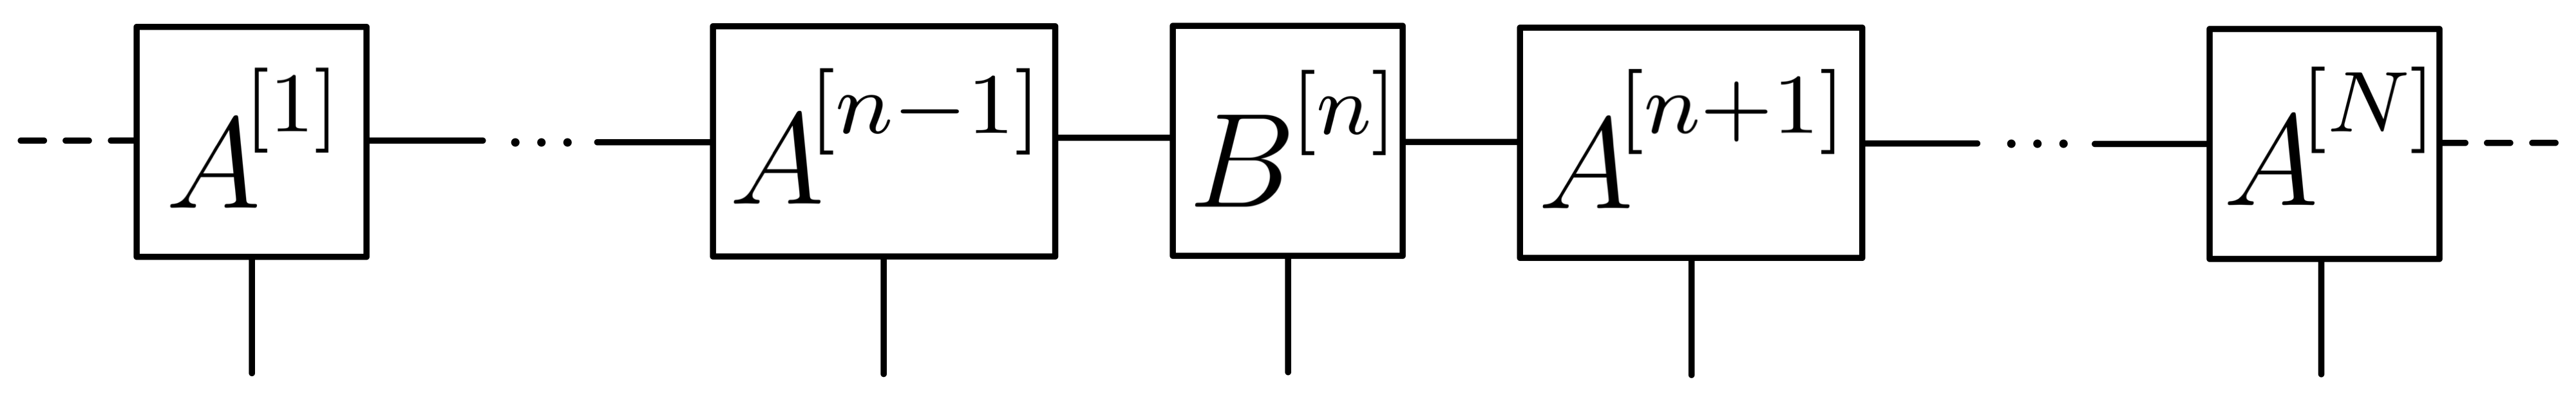
\includegraphics[height=1.2cm]{tangent_vector.png}} \hspace{0.2em}.
\end{split}
\end{align}
But let us first bring the MPS into canonical form, which can always be achieved within the gauge freedom. Note that in this chapter $A$ and $B$ always have to be understood as a set of tensors $\{A^{[n]}\}_{n=1}^N$ and $\{B^{[n]}\}_{n=1}^N$.


% CANONICAL FORM
\section{Intrinsic canonical form}
Our starting point is the general MPS form \eqref{eq:mps}. We initialize the dummy matrix $L^{[N+1]} = ((1)) \in \mathbb{C}^{1 \times 1}$ and successively perform the following LQ decompositions from right to left, i.e. for $n = N, \ldots, 1$:
\begin{equation} \label{eq:mps_canonical_form_lq}
	\raisebox{-0.57\height}{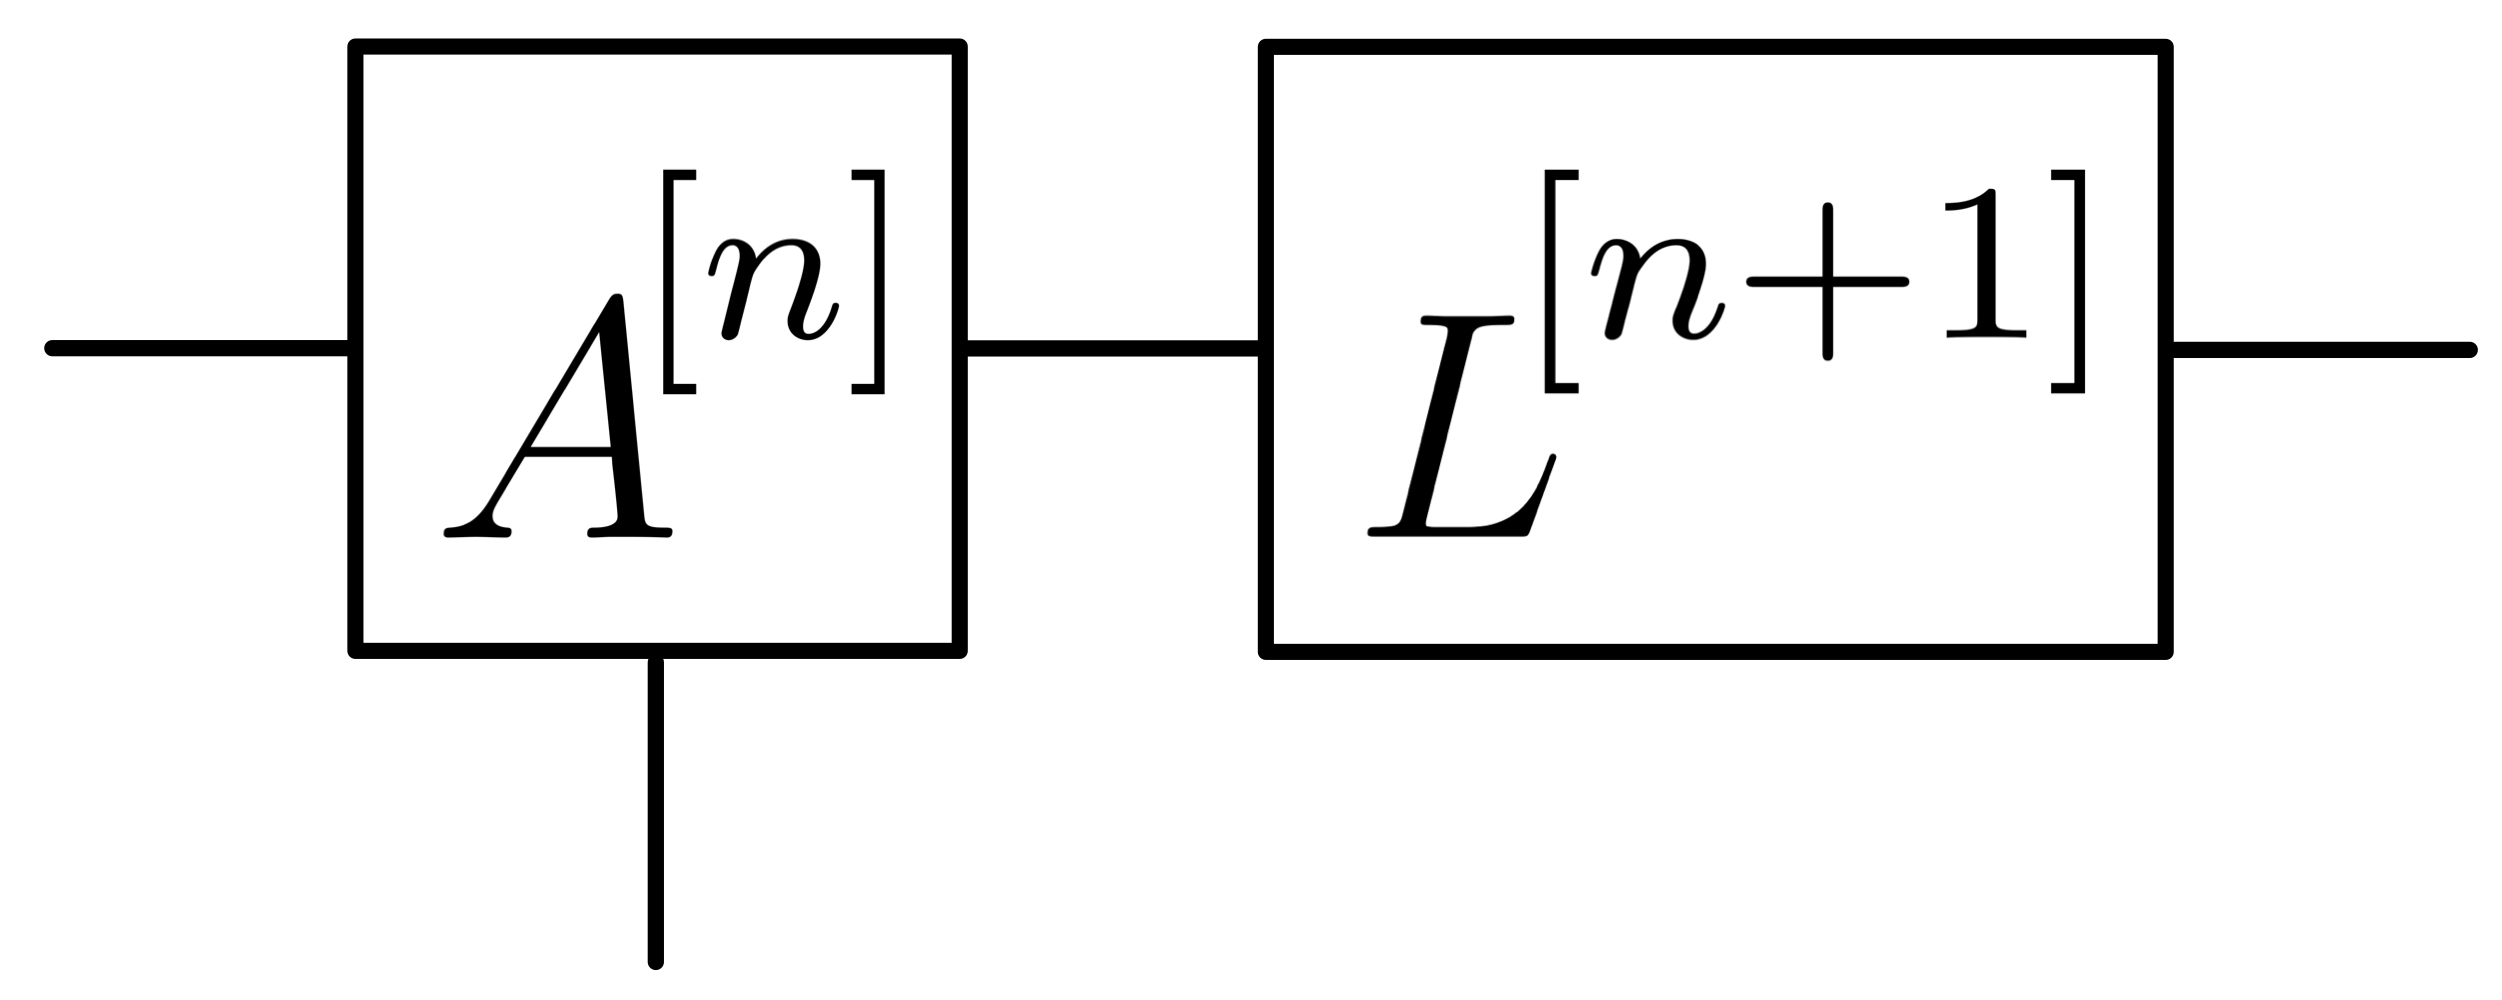
\includegraphics[height=1.3cm]{A_L.png}}
	 \hspace{0.2em} \overset{\mathrm{LQ}}{=} \hspace{0.2em}
	\raisebox{-0.57\height}{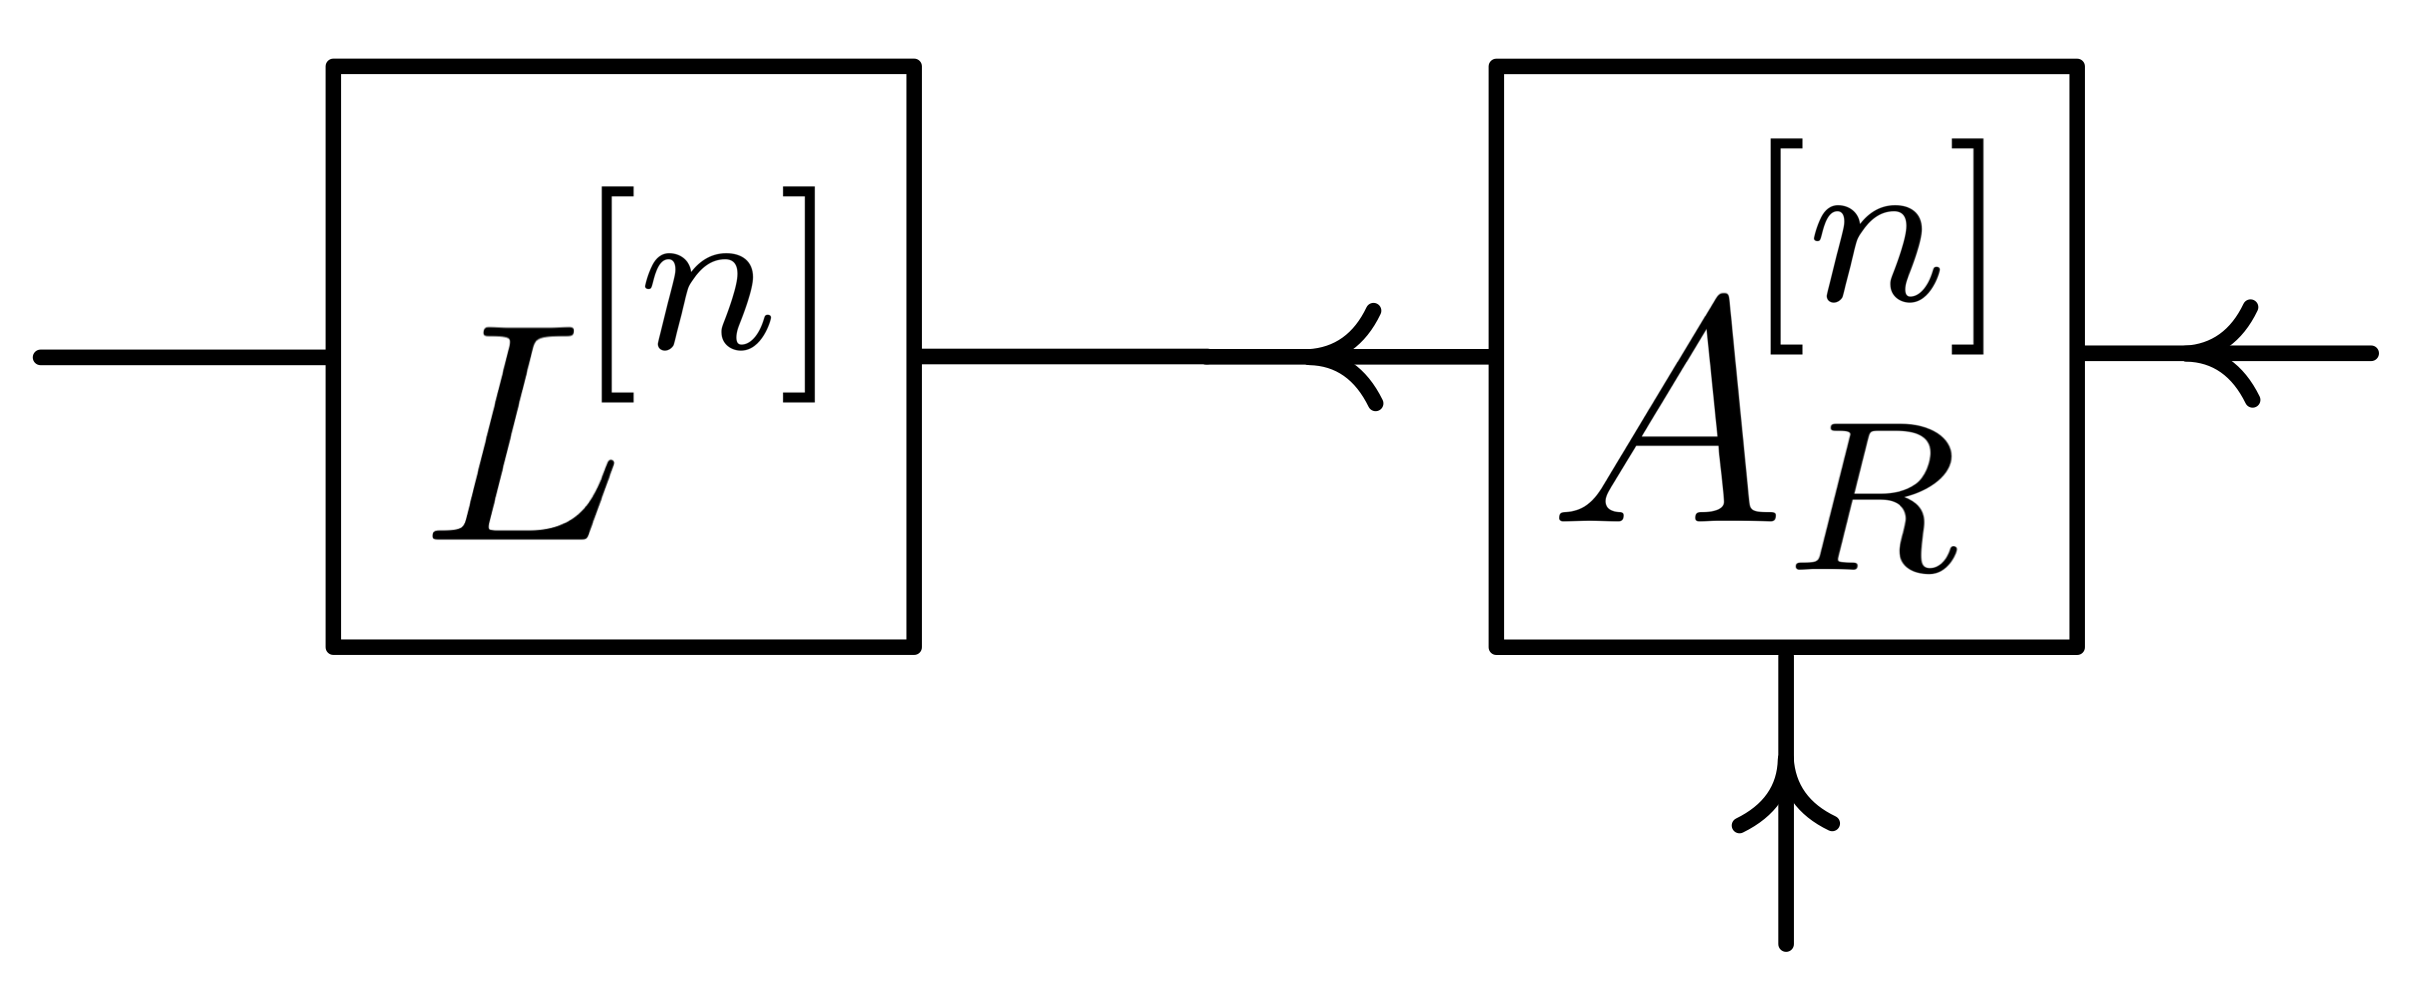
\includegraphics[height=1.3cm]{L_AR.png}} \hspace{0.2em} ,
\end{equation}
where we extract the \textit{right isometric} $A_R^{[n]}$. Since we make the LQ decompositions unique (with positive entries on the main diagonal of the lower triangular matrices $L^{[n]}$), the final $L^{[1]} \in \mathbb{C}^{1 \times 1}$ is positive and equal to the norm of the MPS. In total, the normalized MPS in right isometric form reads
\begin{equation} \label{eq:right_isometric_form_mps}
	\ket{\psi (A)} 
	\hspace{0.2em} = \hspace{0.2em}
	\raisebox{-0.57\height}{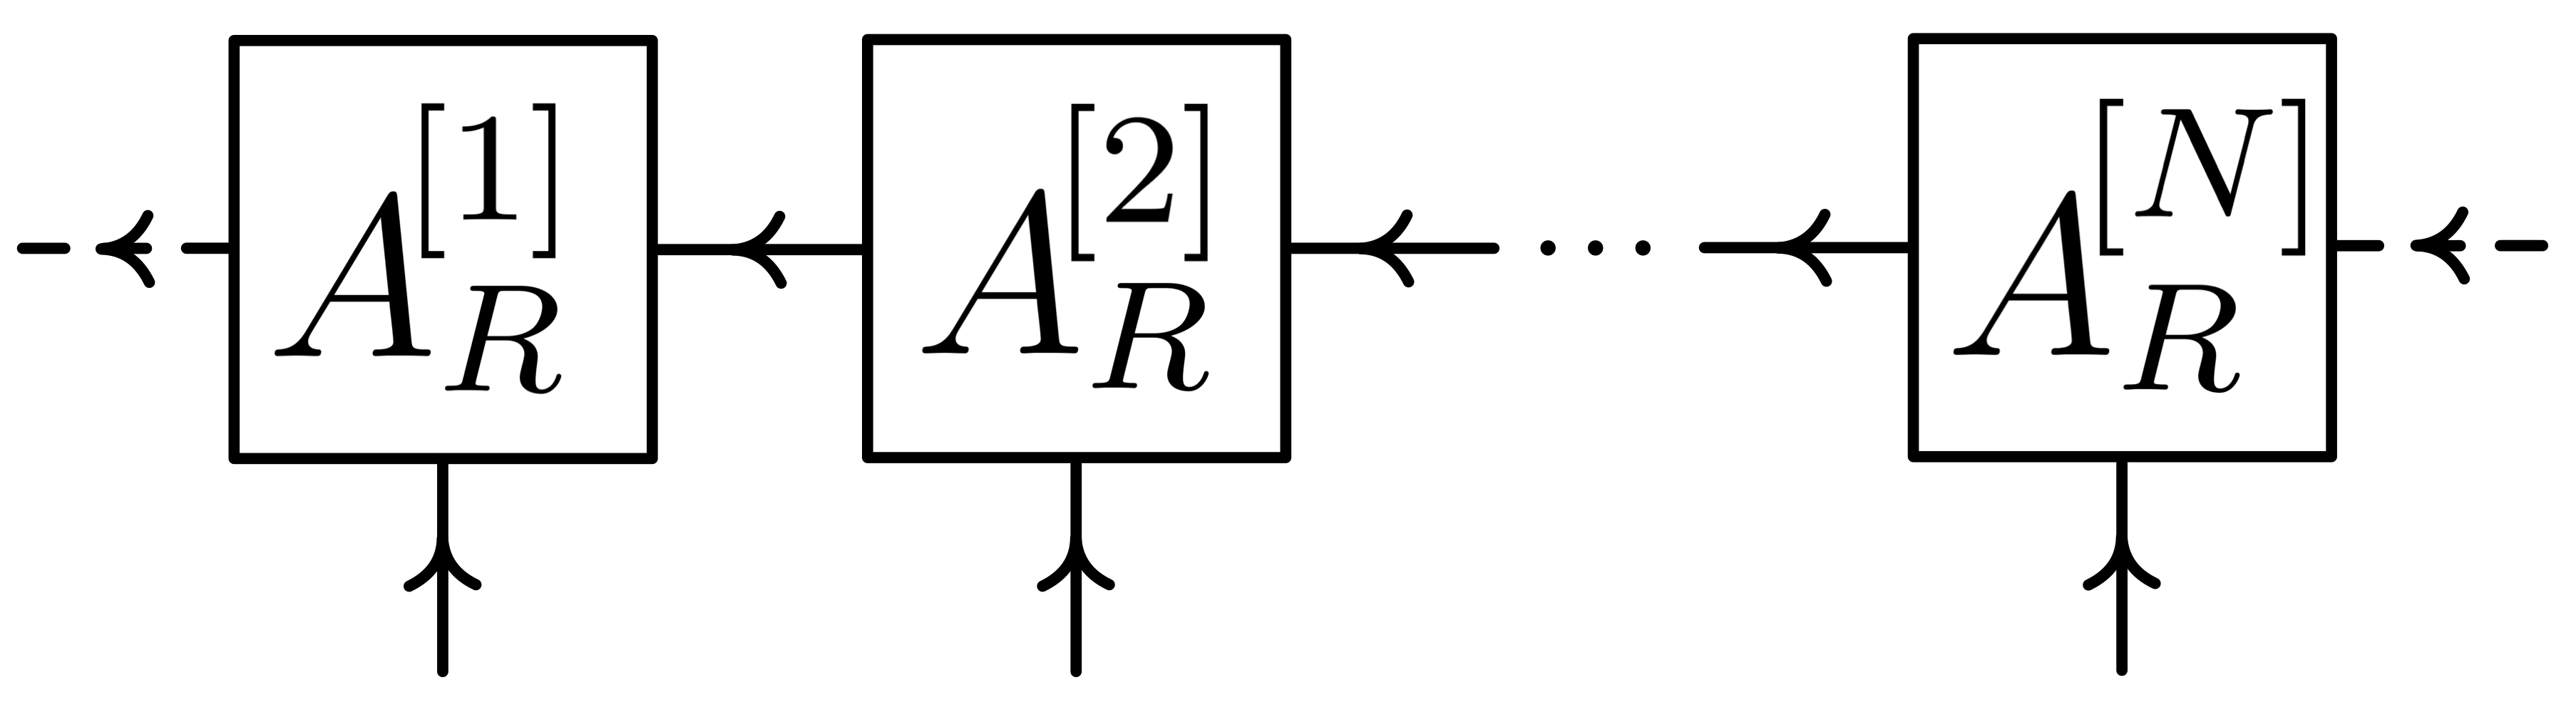
\includegraphics[height=1.3cm]{mps_right_isometric.png}} \hspace{0.2em} .
\end{equation}
Now, we start from the left end of the chain, with dummy matrix $C^{[0]} = ((1)) \in \mathbb{C}^{1 \times 1}$, and perform the following SVDs for $n = 1, \ldots, N$:
\begin{equation} \label{eq:mps_canonical_form_svd}
	\raisebox{-0.57\height}{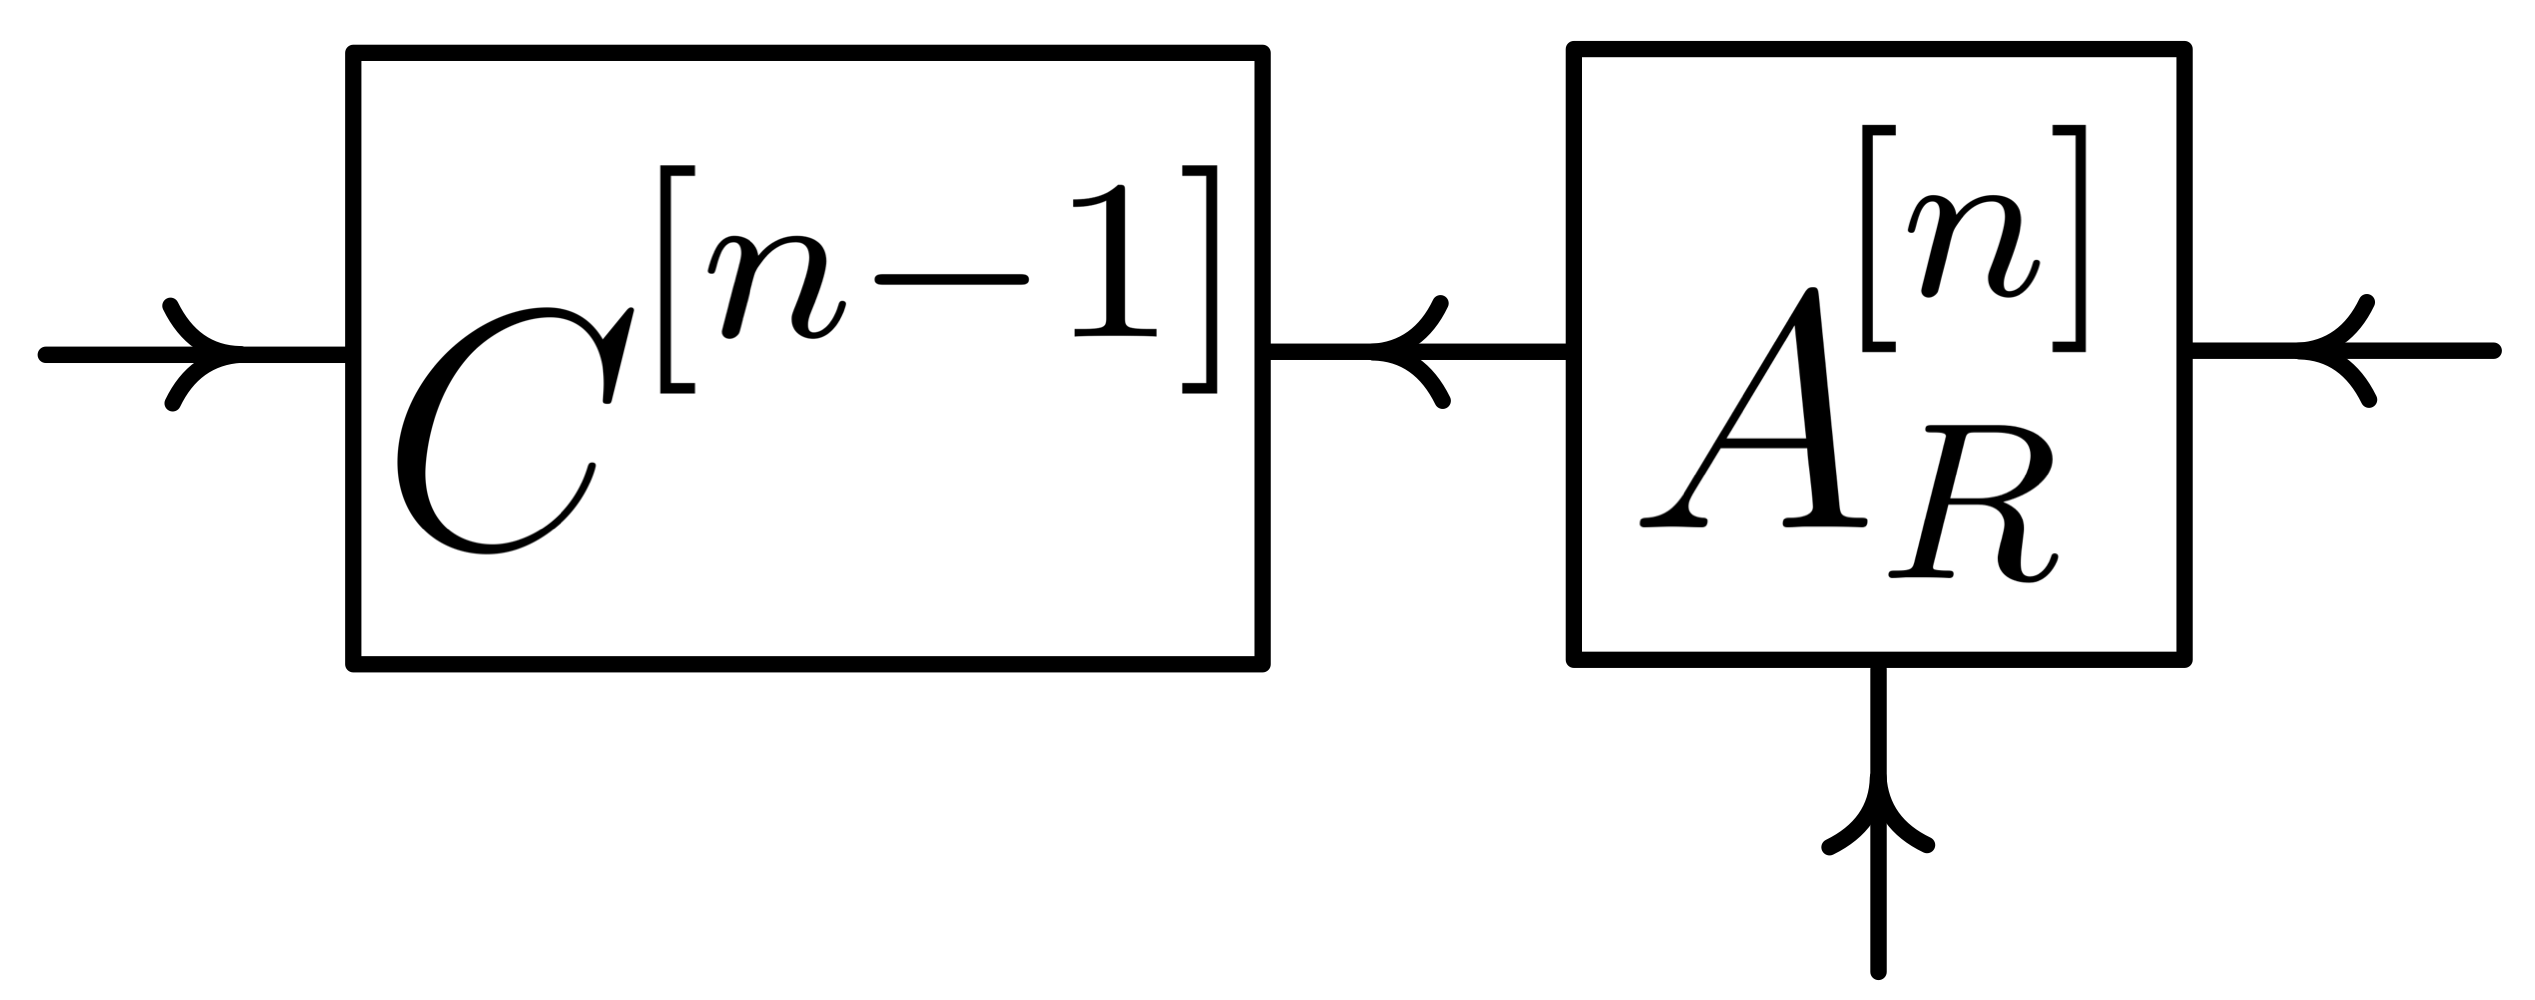
\includegraphics[height=1.3cm]{C_AR.png}}
	 \hspace{0.2em} \overset{\mathrm{SVD}}{=} \hspace{0.2em}
	\raisebox{-0.57\height}{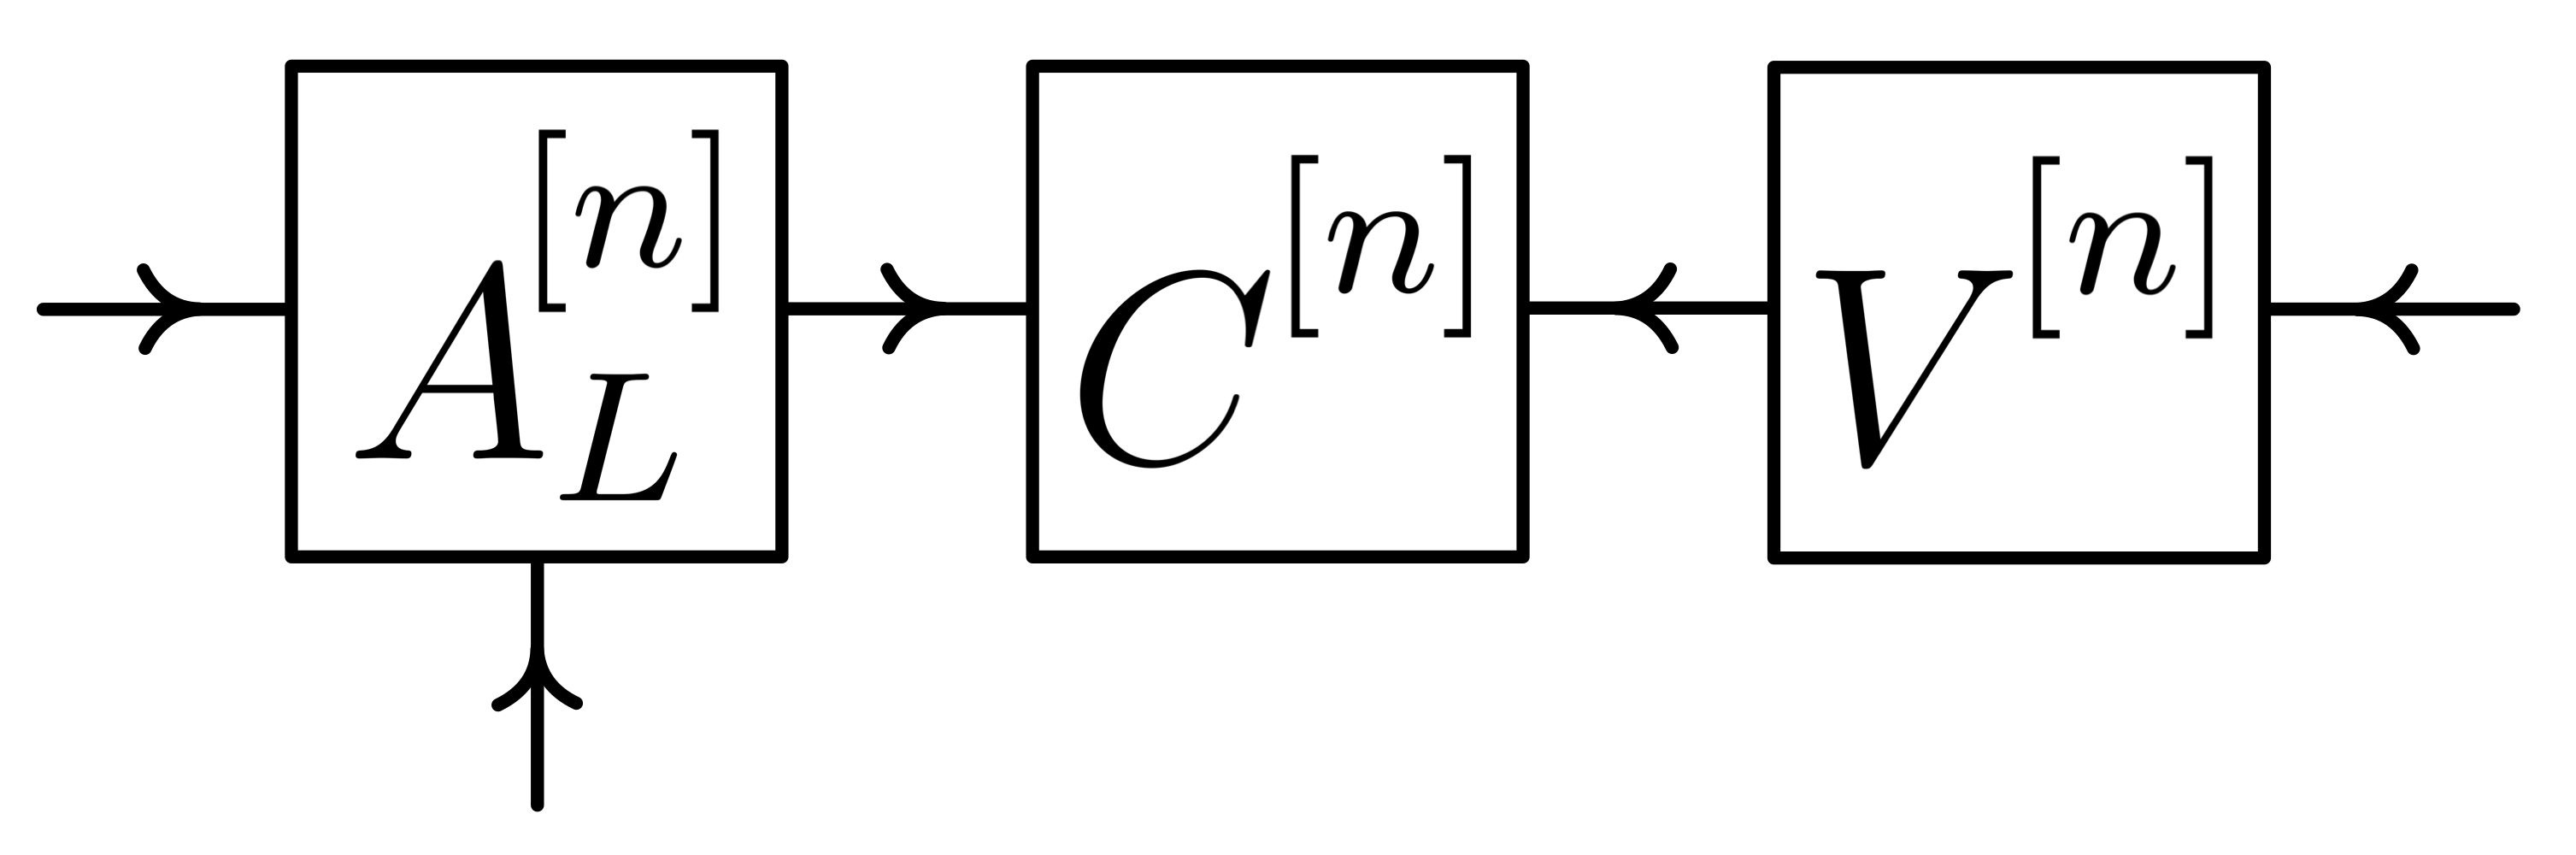
\includegraphics[height=1.3cm]{AL_C_V.png}} \hspace{0.2em},
\end{equation}
with \textit{left isometric tensor} $A_L^{[n]}$ and normalized, diagonal, positive semidefinite \textit{center matrix} $C^{[n]}$. To stay consistent with the right isometric form, we redefine for all $n < N$:
\begin{equation}
	\raisebox{-0.57\height}{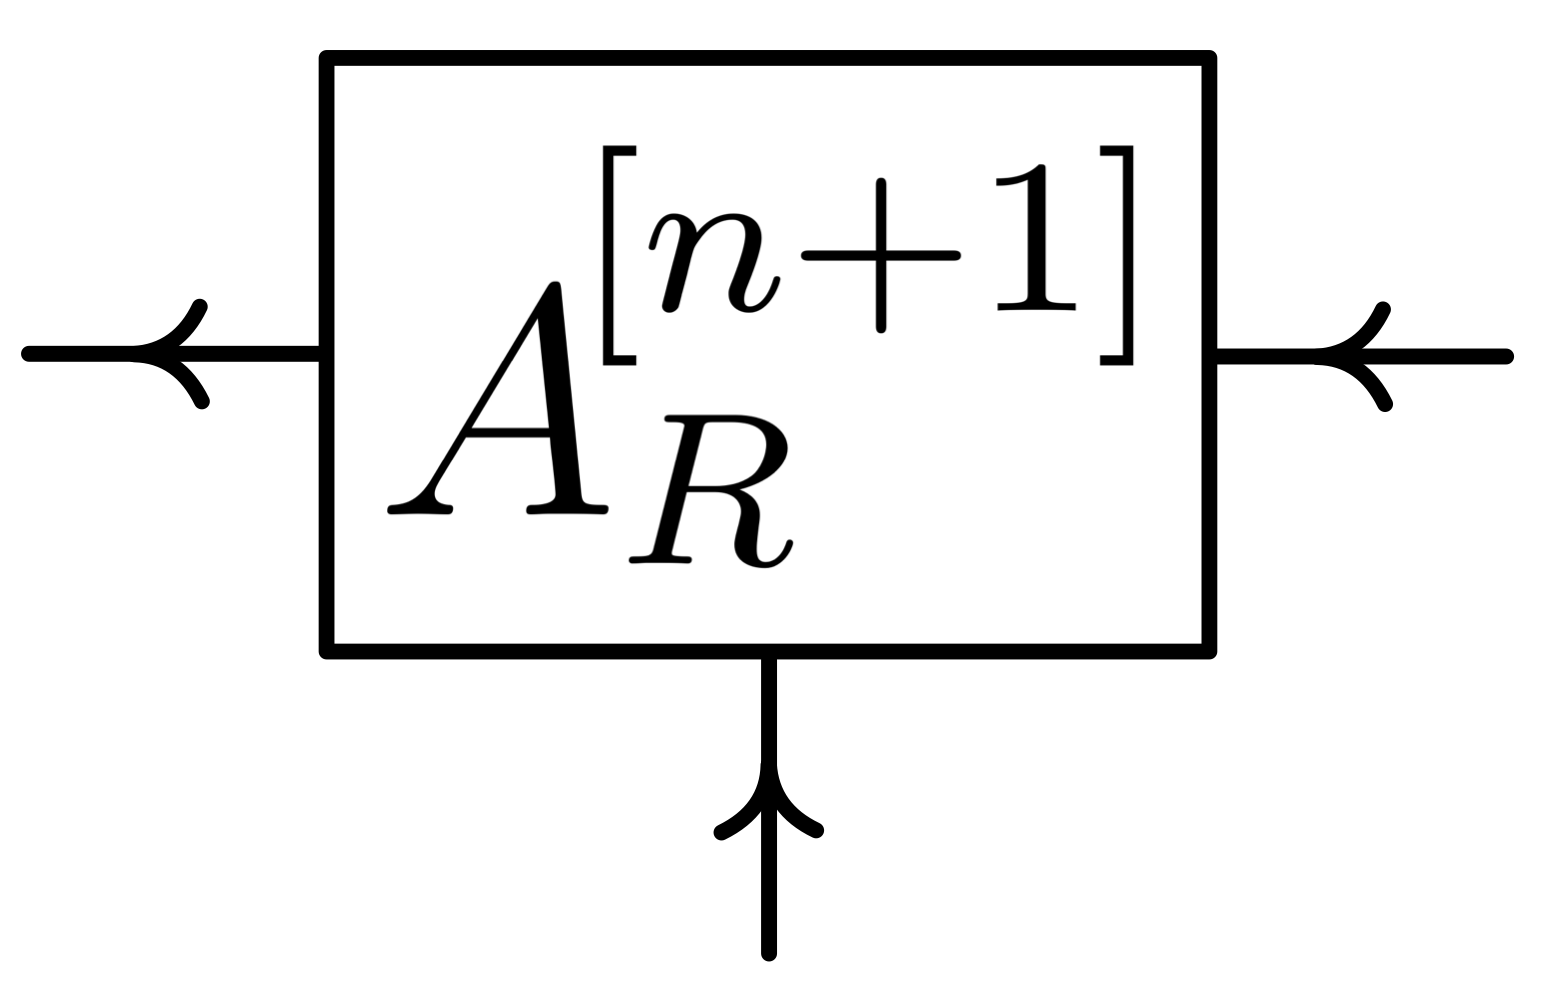
\includegraphics[height=1.3cm]{ARp1.png}}
	\hspace{0.2em} \rightarrow \hspace{0.2em} \hspace{0.2em}
	\raisebox{-0.57\height}{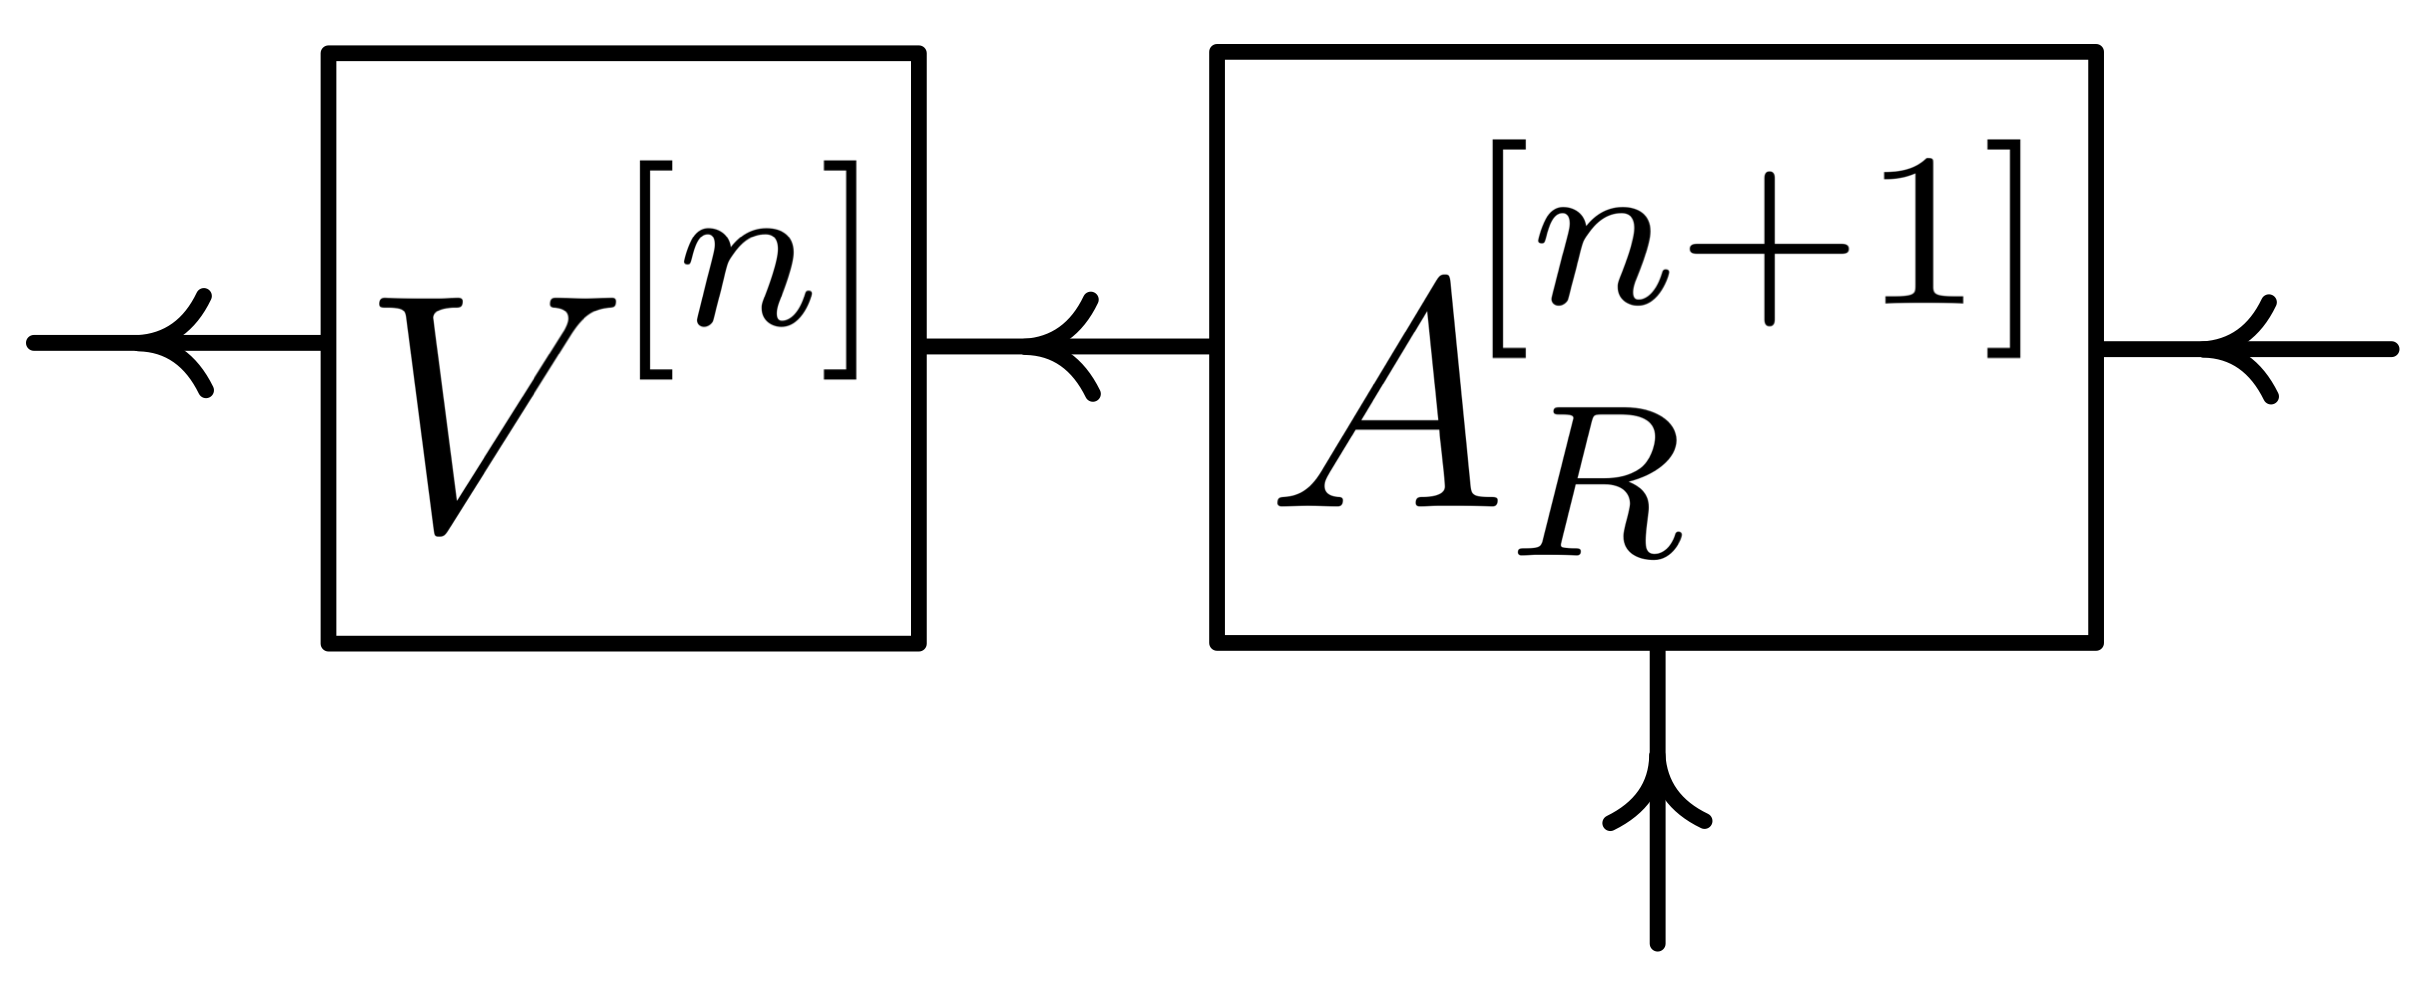
\includegraphics[height=1.3cm]{ARp1_new.png}} \hspace{0.2em},
	\hspace{1em}
	\raisebox{-0.57\height}{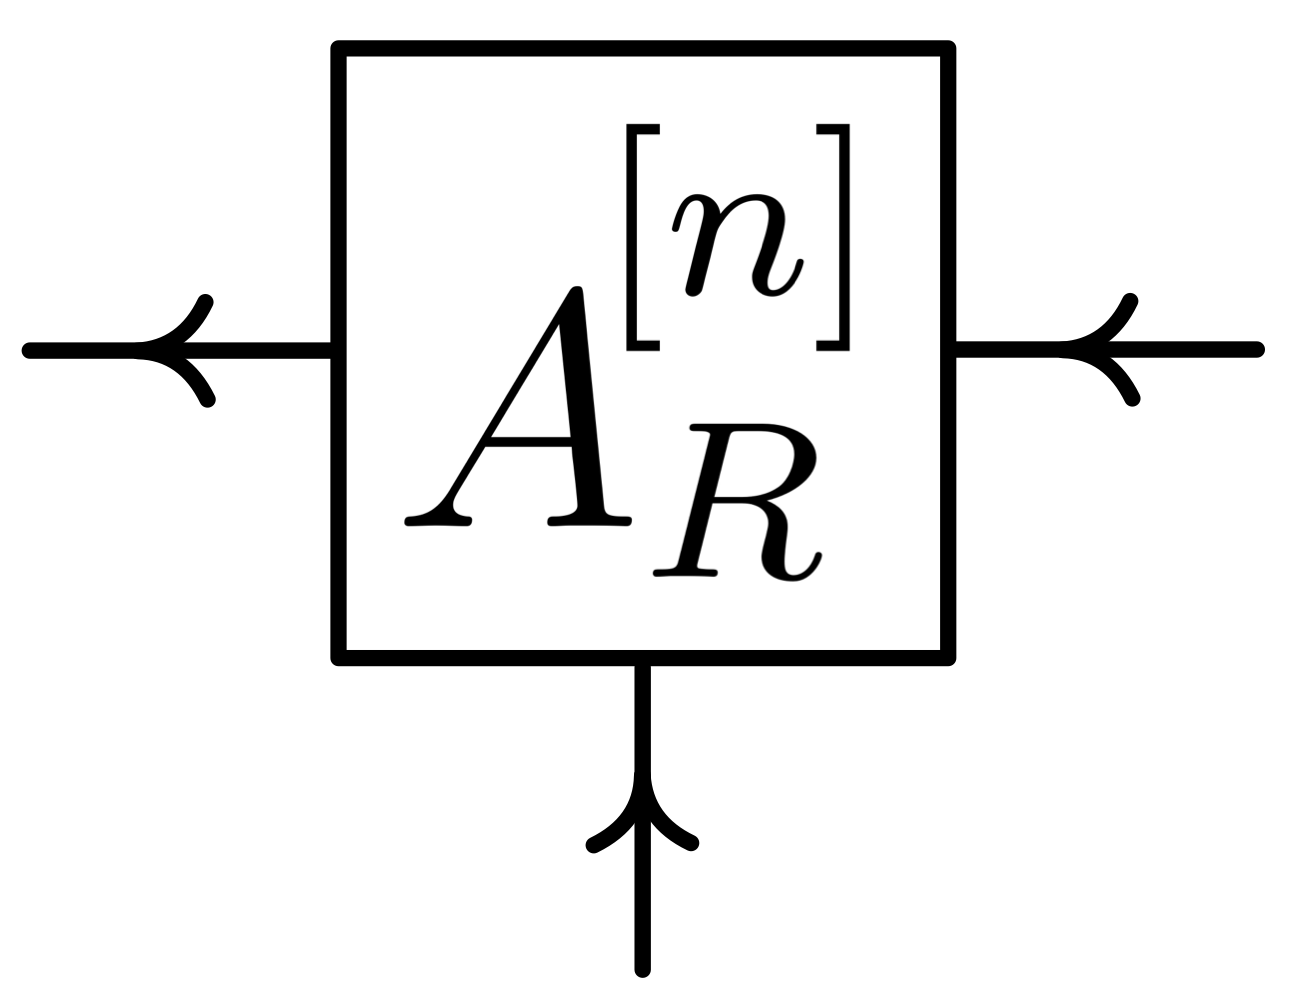
\includegraphics[height=1.3cm]{AR.png}}
	\hspace{0.2em} \rightarrow \hspace{0.2em} \hspace{0.2em}
	\raisebox{-0.57\height}{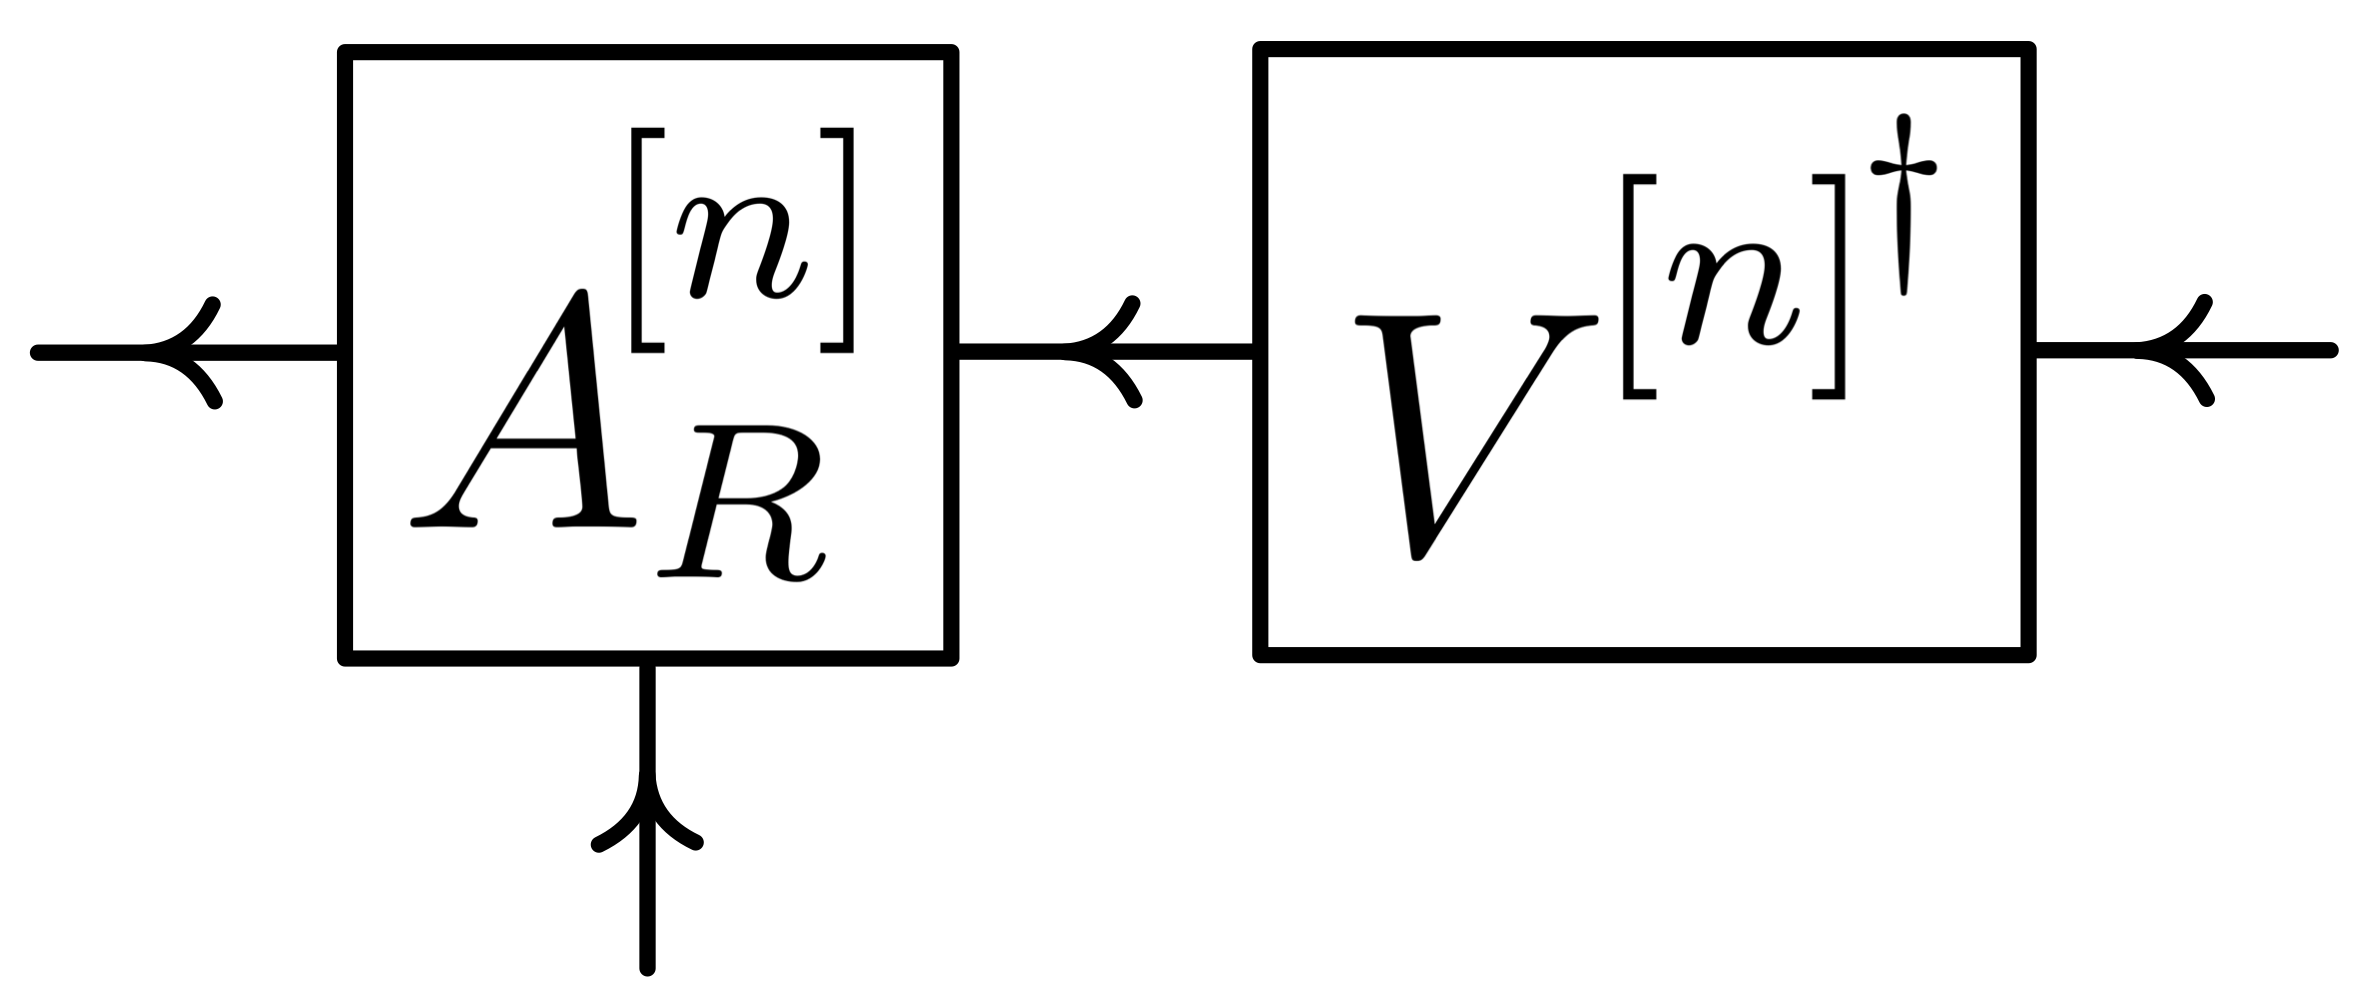
\includegraphics[height=1.3cm]{AR_new.png}} \hspace{0.2em}.
\end{equation}
Sometimes it is convenient to contract $A_L^{[n]}$ and $C^{[n]}$ (or equivalently $C^{[n-1]}$ and $A_R^{[n]}$) into a normalized \textit{center tensor} $A_C^{[n]}$. With this can write the MPS in the following three equivalent ways, for any site $n$ in the chain:
\begin{align} \label{eq:canonical_form_mps}
\begin{split}
	\ket{\psi ( A )} 
	\hspace{0.2em} &= \hspace{0.2em}
	\raisebox{-0.57\height}{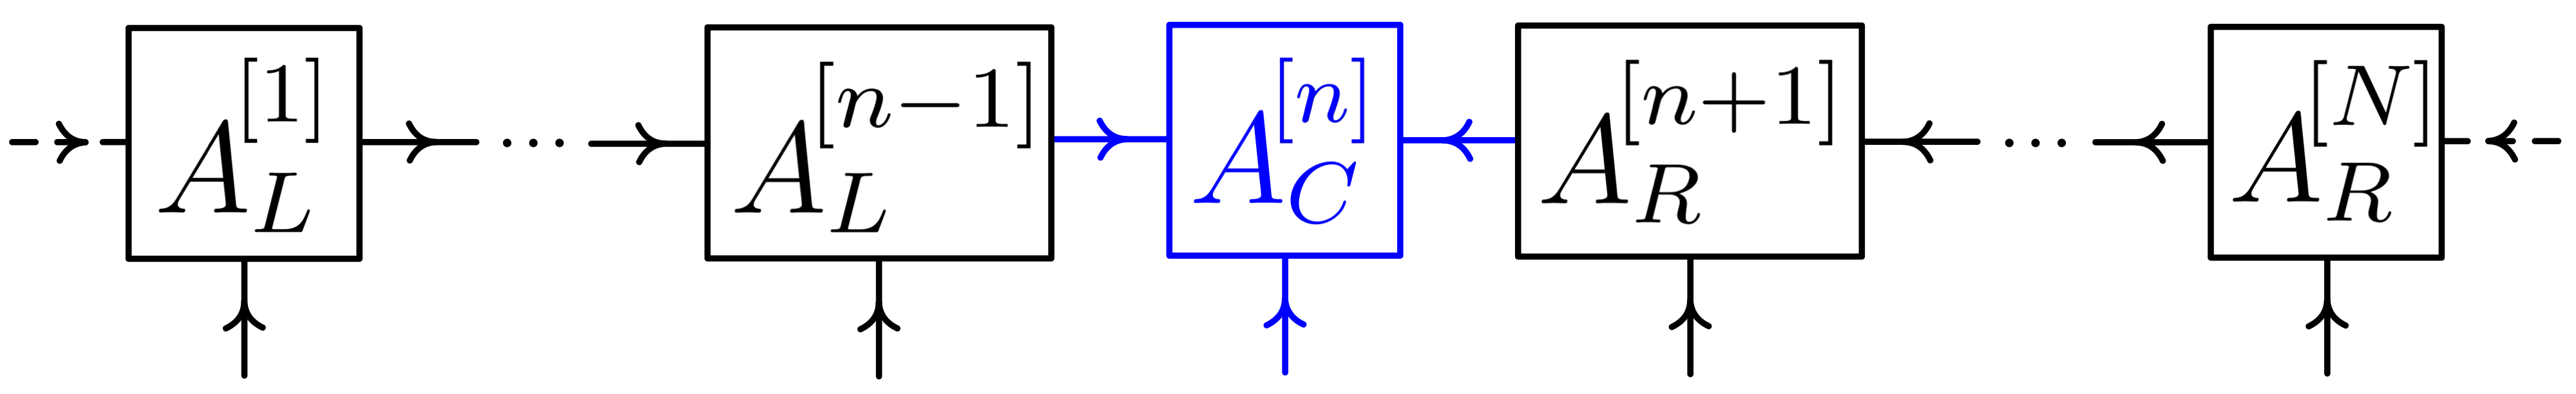
\includegraphics[height=1.3cm]{mps_canonical_1.png}} \\
	\hspace{0.2em} &= \hspace{0.2em}
	\raisebox{-0.57\height}{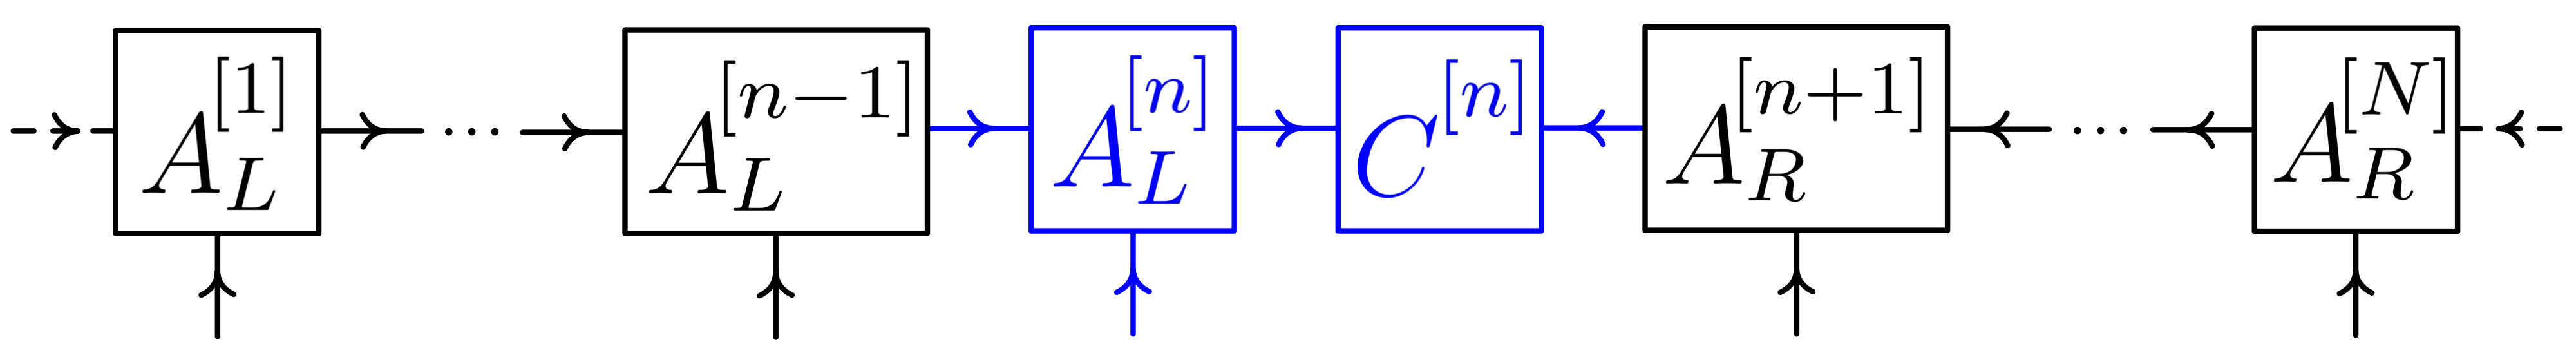
\includegraphics[height=1.3cm]{mps_canonical_2.png}} \\
	\hspace{0.2em} &= \hspace{0.2em}
	\raisebox{-0.57\height}{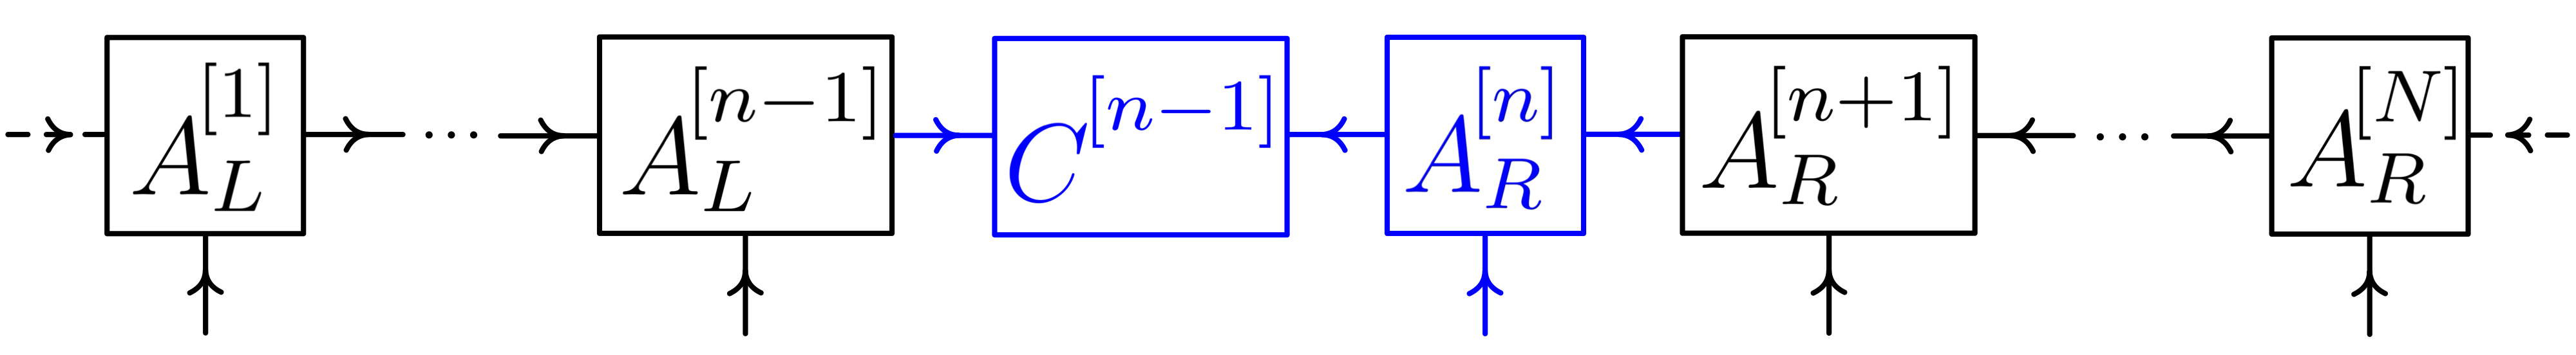
\includegraphics[height=1.3cm]{mps_canonical_3.png}} \hspace{0.2em}.
\end{split}
\end{align}
\noindent This is the \textit{canonical form} for MPS, the finite analog of \eqref{eq:umps_canonical_form}. In particular, it gives direct access to the Schmidt values, on the diagonal of $C^{[n]}$ for a bipartition at bond $n$. This clarifies the restriction of the tensor manifold to positive definite virtual density matrices \eqref{eq:virtual_density_matrices}. In canonical form, they simply become $l^{[n]} = (C^{[n]})^2$ and $r^{[n]} = \mathbbm{1}$, so that positive definiteness becomes equivalent to full Schmidt rank. \\[0.5em]
\noindent At this point, let us also specify the values of the bond dimensions $\{ D_n \}_{n=1}^{N-1}$, appearing in the tensor dimensions as
\begin{equation}
	A_L^{[n]}, A_R^{[n]}, A_C^{[n]} \in \mathbb{C}^{D_{n-1} \times d \times D_n}, \: C^{[n]} \in \mathbb{C}^{D_n \times D_n}.
\end{equation}
In principle, any state $\ket{\psi} \in \mathbb{C}^{d^N}$ can be brought into right isometric MPS form \eqref{eq:right_isometric_form_mps} with successive LQ decompositions. In the generic case, the bond dimensions then satisfy $D_n = \mathrm{min} (d^n, d^{N-n})$ and thus grow exponentially from both sides until they reach $d^{\lfloor N/2 \rfloor}$ in the middle of the chain. However, the area law \eqref{eq:area_law} tells us that ground states of local, gapped Hamiltonians can be faithfully approximated using bond dimensions that remain non-extensive in system size. Accordingly, we impose an upper bound $D_{\text{max}}$ in practical computations:
\begin{equation} \label{eq:bond_dimensions_mps}
	D_n = \mathrm{min} (d^n, d^{N-n}, D_{\mathrm{max}}).
\end{equation}

% DMRG
\section{Density matrix renormalization group (DMRG)} \label{sec:dmrg}
\noindent To minimize the Hamiltonian energy for the MPS in canonical form \eqref{eq:canonical_form_mps}, we want to optimize one center tensor at a time, while keeping all the other isometric tensors fixed. An obvious choice for the center tensor is $A_C^{[n]}$, which leads to the \textit{one site density matrix renormalization group} algorithm. Dependent on the chosen initial state, this variational method is quite prone to getting stuck. The bond dimensions stay fixed throughout the whole optimization, so one is restricted to a single, potentially suboptimal manifold. To circumvent this, we enlarge the center by $A_R^{[n+1]}$ to a two-site tensor which we call $\theta_2^{[n, n+1]}$:
\begin{equation} \label{eq:mps_theta2}
	\ket{\psi ( A )} 
	\hspace{0.2em} = \hspace{0.2em}
	\raisebox{-0.37\height}{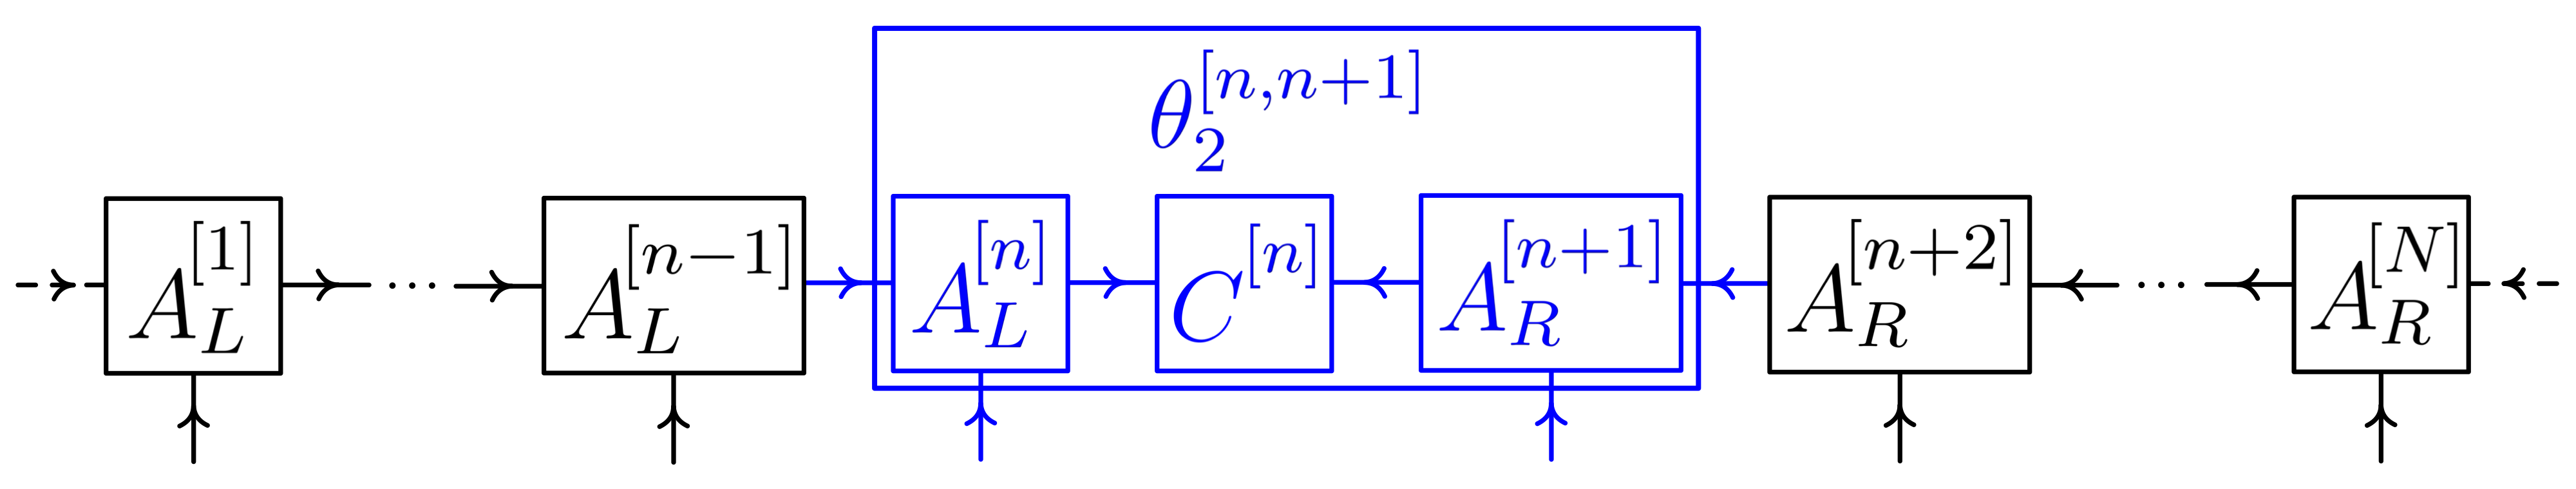
\includegraphics[height=2cm]{mps_canonical_theta2.png}} \hspace{0.2em} .
\end{equation}
This is the variational state for the \textit{two site density matrix renormalization group} algorithm \cite{schollwock2011density}. Let us next express the Hamiltonian in a form that matches the MPS structure. \\[1em]

% mpo Hamiltonian
\noindent \underline{MPO Hamiltonian} \\[0.5em]
\noindent In the same way we can represent any state $\ket{\psi} \in \mathbb{C}^{d^N}$ as an MPS, we can represent any Hamiltonian $H \in \mathbb{C}^{d^N \times d^N}$ as a \textit{matrix product operator} (MPO). More precisely, we can find $N$ four leg tensors 
\begin{equation}
	W^{[n]} \in \mathbb{C}^{\chi_{n-1} \times \chi_{n} \times d \times d} \text{ with } \chi_0 = \chi_N = 1,
\end{equation}
such that
\begin{equation} \label{eq:mpo}
	H = \sum_{\{s_n\}} \sum_{\{\Tilde{s}_n\}} W^{[1] s_1, \Tilde{s}_1} W^{[2] s_2, \Tilde{s}_2} \cdots W^{[N] s_N, \Tilde{s}_N} \ket{s_1 \ldots s_N} \bra{\Tilde{s}_1 \ldots \Tilde{s}_N} 
	= \raisebox{-0.44\height}{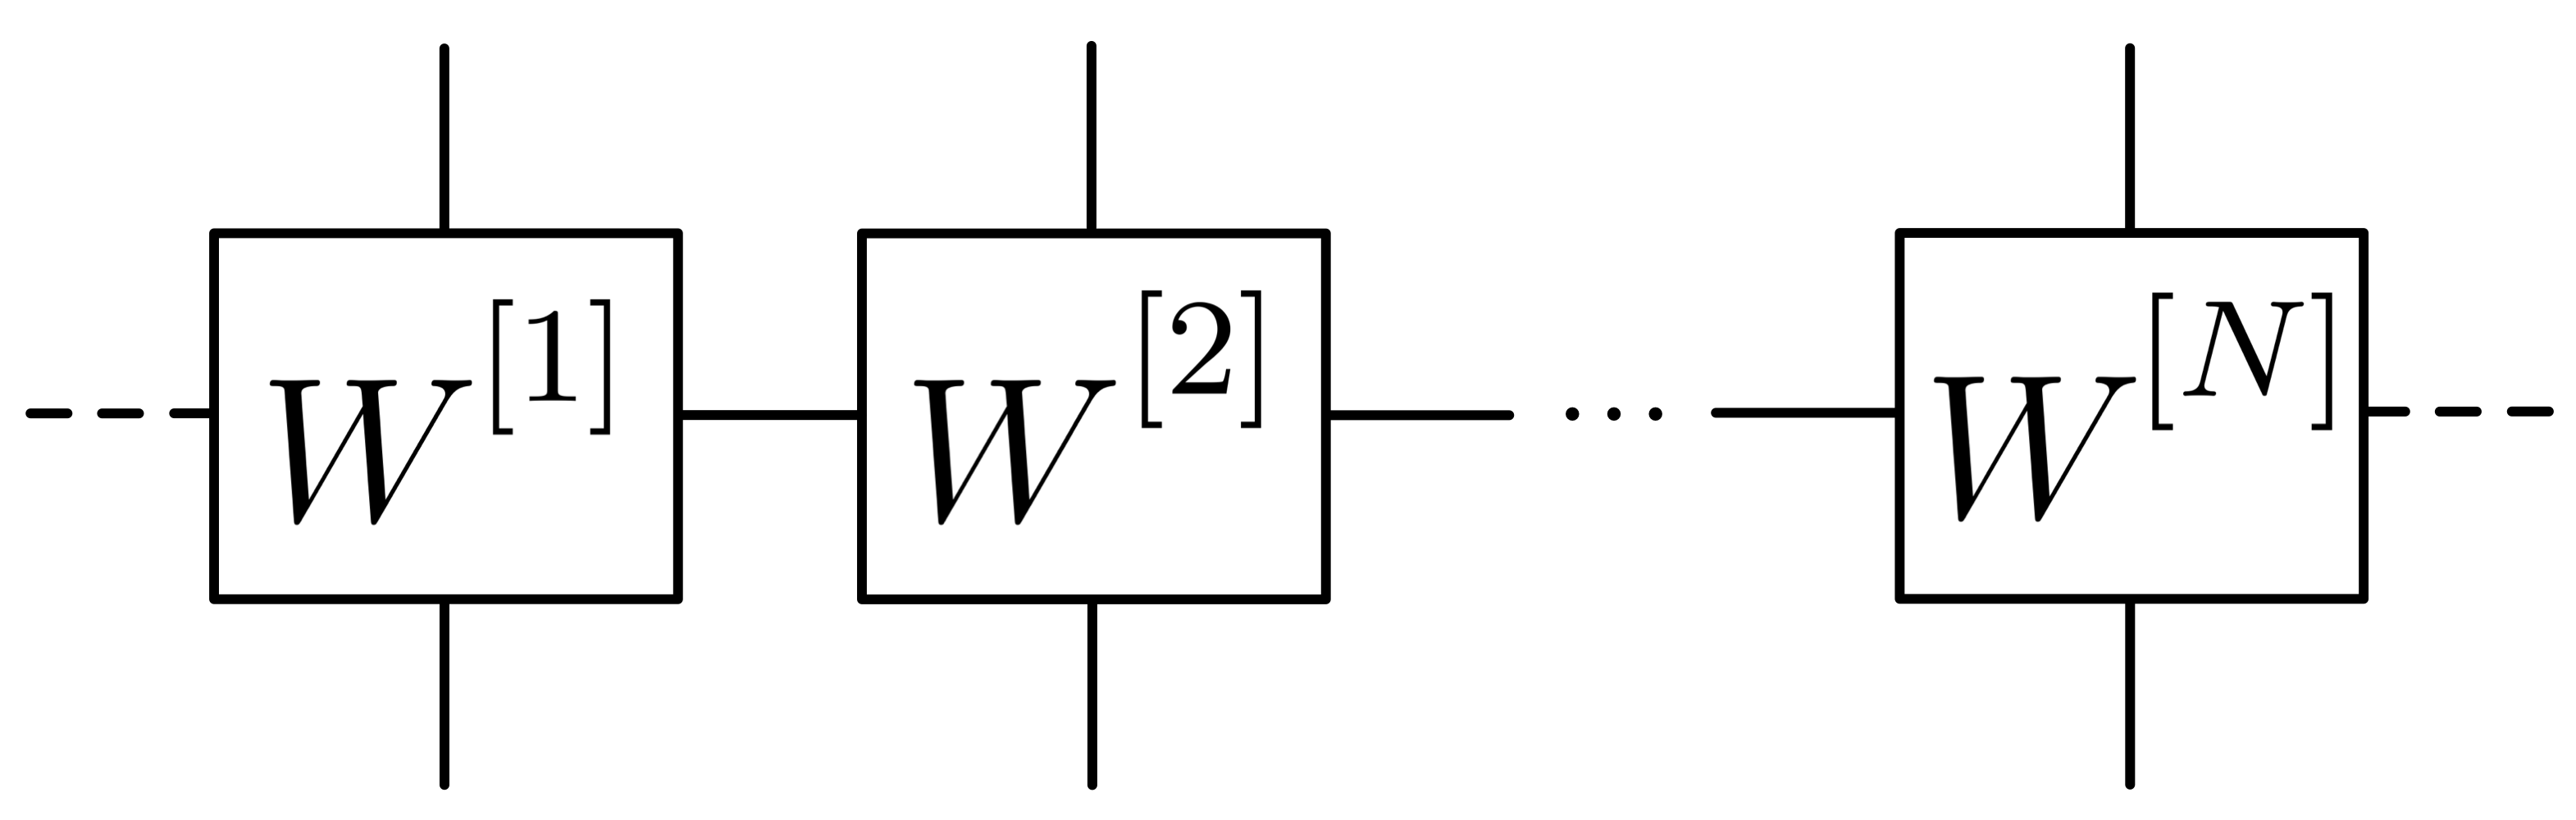
\includegraphics[height=1.7cm]{mpo.png}} \hspace{0.2em} .
\end{equation}
The key limitation for efficient algorithms involving such MPOs lies in the bond dimensions $\chi_{n}$. In the worst case, they scale exponentially in system size $N$. This is not the case for local Hamiltonians, which we want to demonstrate for the transverse field Ising model. Since our MPS \eqref{eq:canonical_form_mps} has open boundary conditions by construction, they are the most natural choice for the Hamiltonian as well. \\[0.75em]
\noindent 1) Open boundary conditions (OBC) \\[0.5em]
We start from the Hamiltonian in the normal form, namely as a sum of Kronecker products involving $N$ spin operators each:
\begin{align} \label{eq:1d_tfi_obc}
\begin{split}
	H = -J \sum_{n=1}^{N-1} \sigma^x_n \sigma^x_{n+1} - g \sum_{n=1}^N \sigma^z_n 
	= & \hspace{0.5em} 
	\sigma^x \otimes (-J \sigma^x) \otimes \mathbbm{1} \otimes \cdots \otimes \mathbbm{1} \\[-0.4em]
	& + \hspace{0.5em} 
	(- g \sigma^z) \otimes \mathbbm{1} \otimes \cdots \otimes \mathbbm{1} \\[0.5em]
	&+ \hspace{0.5em}
	\mathbbm{1} \otimes \sigma^x \otimes (-J \sigma^x) \otimes \mathbbm{1} \otimes \cdots \otimes \mathbbm{1} \\[0.5em]
	& + \hspace{0.5em} 
	\mathbbm{1} \otimes (- g \sigma^z) \otimes \mathbbm{1} \otimes \cdots \otimes \mathbbm{1} \\[0.5em]
	& + \hspace{0.5em} \ldots \hspace{0.5em} .
\end{split}
\end{align}
To derive the corresponding MPO, it is useful to start a so called \textit{final state machine} (FSM) \cite{motruk2016density}. It is a graph whose nodes represent states and whose directed edges indicate transitions between those states. In the \textit{ready state} $R$ no nontrivial operator has yet been applied, in the \textit{final state} $F$ a whole nontrivial action has been completed. For every summand in the Hamiltonian, there is one path from the leftmost ready state to the rightmost final state, consisting of $N$ transitions. Every transition adds a spin operator to the Kronecker product. As an example, let us consider the interaction term $-J \sigma^x_1 \otimes \sigma^x_2$ between the first two spins. We transition from $R$ to $X_1$ by applying $\sigma^x$ on the first site. The transition from $X_1$ to $F$ completes the interaction with the application of the operator $-J \sigma^x$ on site 2. The rest of the path consists of $F$ to $F$ transitions under application of the identity $\mathbbm{1}$. In total we get the following FSM:
\begin{equation}
	\raisebox{-0.4\height}{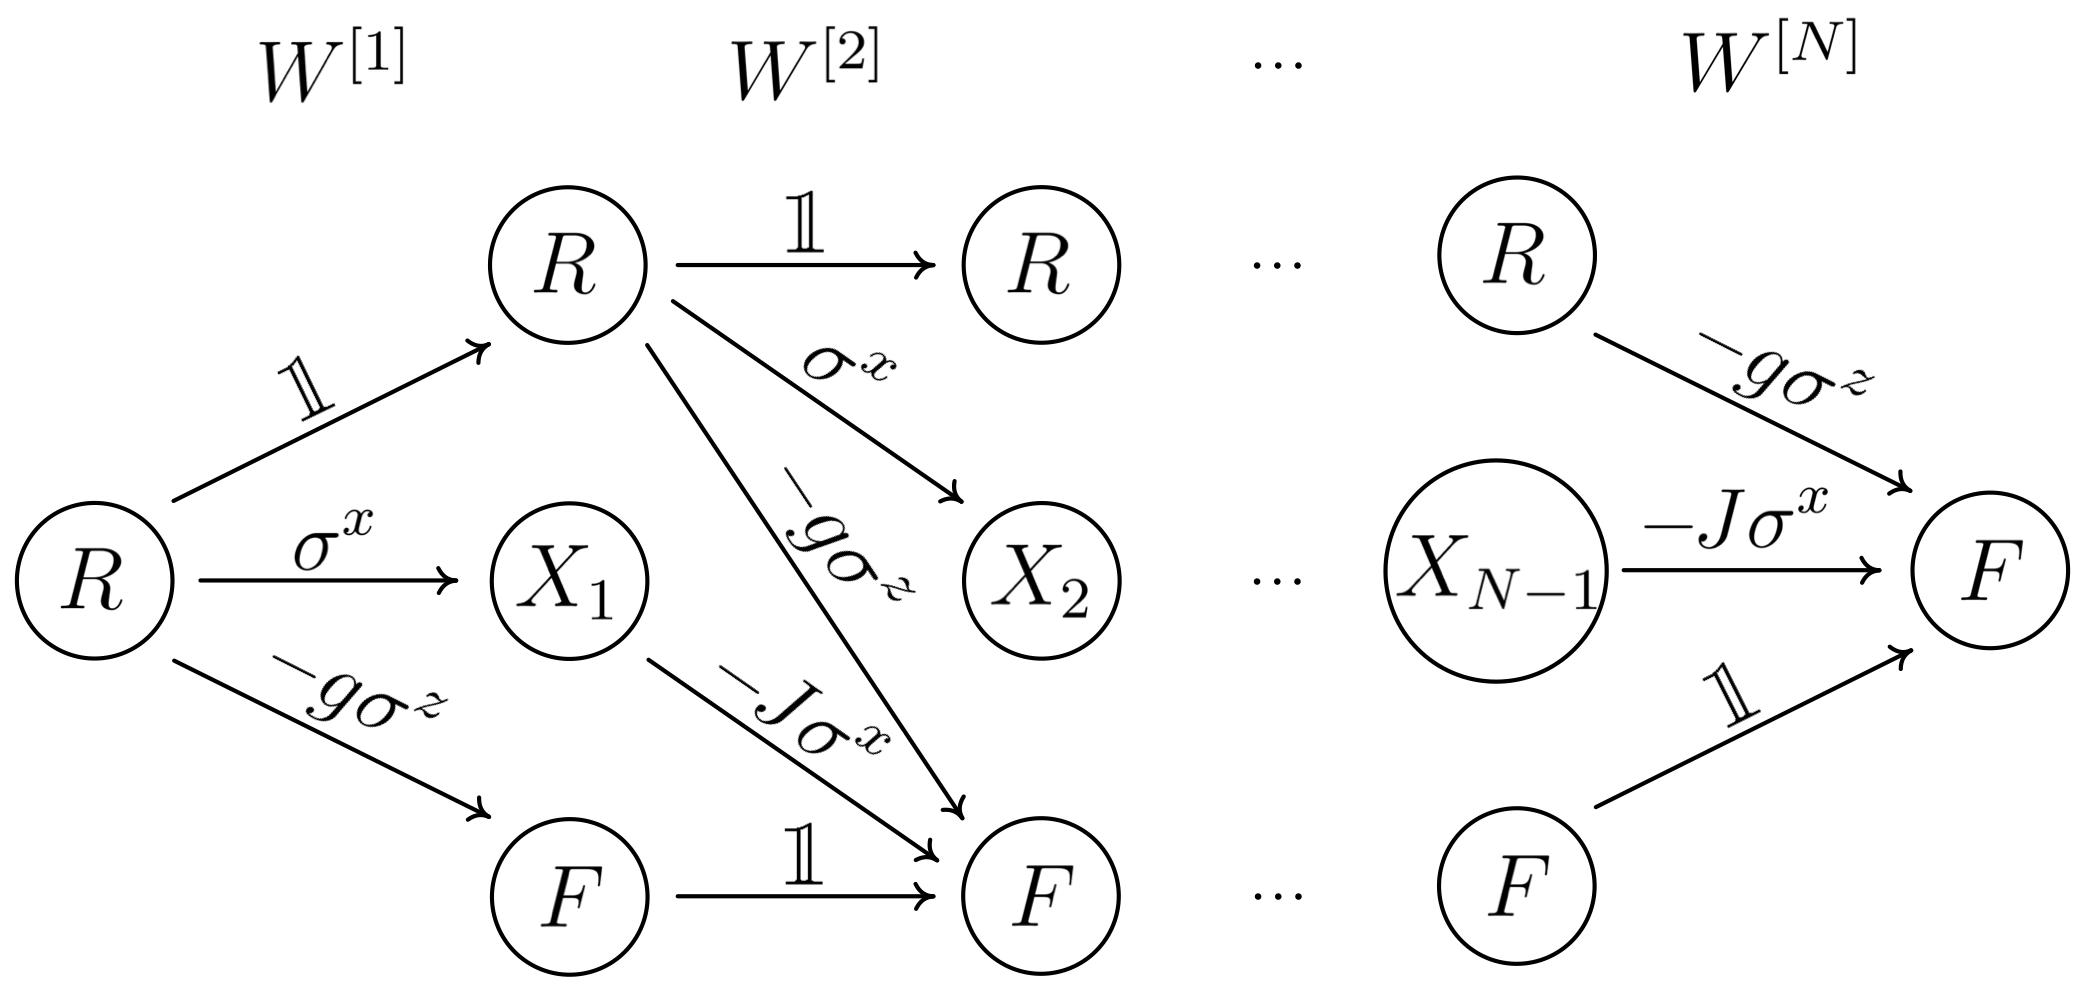
\includegraphics[height=4.5cm]{finite_state_automaton_obc.png}} \:.
\end{equation}
Seeing the four leg tensor $W^{[n]}$ as matrix (virtual legs) with spin operators (physical legs) as entries, the matrix lines are indexed by the states before the transition $n$, the columns by the states afterwards, and the matrix elements are defined by the transition operators. This gives us the following MPO tensors for the Hamiltonian \eqref{eq:1d_tfi_obc}:
\begin{equation} \label{eq:mpo_obc}
	\overset{\raisebox{0.5em}{$W^{[1]}$}}{\begin{pmatrix} \mathbbm{1} & \sigma^x & -g \sigma^z \end{pmatrix}}, 
	\hspace{0.5em}
	\overset{\raisebox{0.5em}{$W^{[2]}, \ldots, W^{[N-1]}$}}{\begin{pmatrix}  \mathbbm{1} & \sigma^x & -g \sigma^z \\ 0 & 0 & -J \sigma^x \\ 0 & 0 & \mathbbm{1} \end{pmatrix}}, 
	\hspace{0.5em}
	\overset{\raisebox{0.5em}{$W^{[N]}$}}{\begin{pmatrix} -g \sigma^z \\ -J \sigma^x \\ \mathbbm{1} \end{pmatrix}}.
\end{equation}
\noindent 2) Periodic boundary conditions (PBC) \\[0.5em]
With regard to the quasiparticle excitations we will create later, we would like to have MPS eigenstates with a definite momentum. In order to commute with the translation operator, the Hamiltonian must have periodic boundary conditions (PBC). In principle, we could also construct the MPS with PBC. But the resulting closed loop in the virtual legs would prevent a canonical form, making the optimization significantly harder. As a practical compromise, we take the Hamiltonian to be periodic and try to restore momentum as a good quantum number for our MPS with open boundaries. The Hamiltonian, finite state machine and MPO tensors for PBC are:
\begin{equation}\label{eq:1d_tfi_pbc}
	H = -J \sum_{n=1}^{N-1} \sigma^x_n \sigma^x_{n+1} - g \sum_{n=1}^N \sigma^z_n - J \sigma^x_N \sigma^x_{1},
\end{equation}
\begin{equation}
	\raisebox{-0.4\height}{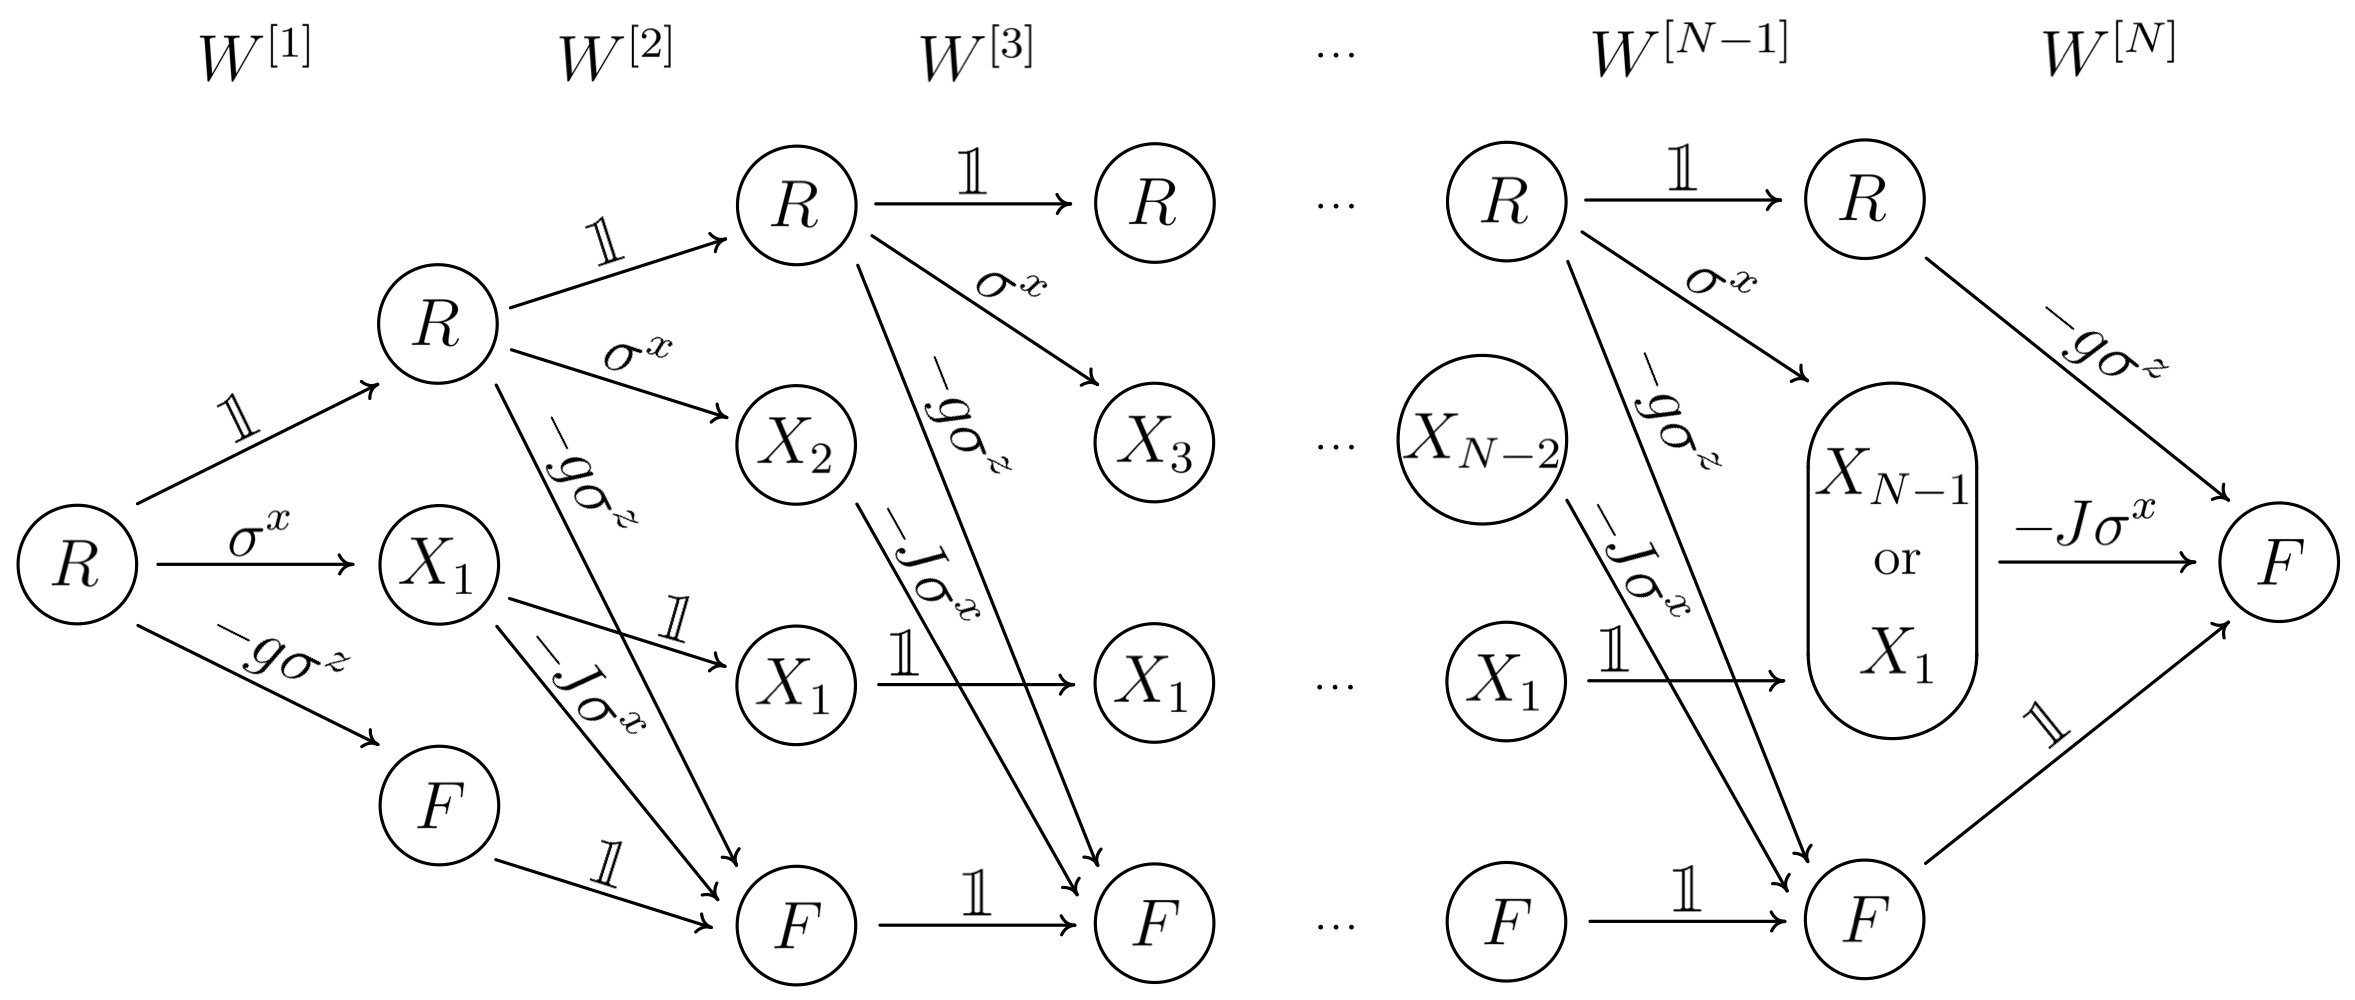
\includegraphics[height=6cm]{finite_state_automaton_pbc.png}} \:,
\end{equation}
\begin{equation} \label{eq:mpo_pbc}
	\overset{\raisebox{0.5em}{$W^{[1]}$}}{\begin{pmatrix} \mathbbm{1} & \sigma^x & -g \sigma^z \end{pmatrix}}, \:\: 
	\overset{\raisebox{0.5em}{$W^{[2]}$}}{\begin{pmatrix}  \mathbbm{1} & \sigma^x & 0 & -g \sigma^z \\ 0 & 0 & \mathbbm{1} & -J \sigma^x \\ 0 & 0 & 0& \mathbbm{1} \end{pmatrix}}, \:\:
	\overset{\raisebox{0.5em}{$W^{[3]}, \ldots, W^{[N-2]}$}}{\begin{pmatrix}  \mathbbm{1} & \sigma^x & 0 & -g \sigma^z \\ 0 & 0 & 0 & -J \sigma^x \\ 0 & 0 & \mathbbm{1} & 0 \\ 0 & 0 & 0& \mathbbm{1} \end{pmatrix}}, \:\:
	\overset{\raisebox{0.5em}{$W^{[N-1]}$}}{\begin{pmatrix}  \mathbbm{1} & \sigma^x & -g \sigma^z \\ 0 & 0 & -J \sigma^x \\ 0 & \mathbbm{1} & 0  \\ 0 & 0& \mathbbm{1} \end{pmatrix}}, \:\:
	\overset{\raisebox{0.5em}{$W^{[N]}$}}{\begin{pmatrix} -g \sigma^z \\ -J \sigma^x \\ \mathbbm{1} \end{pmatrix}}.
\end{equation}

% dmrg
\noindent \underline{DMRG} \\[0.5em]
We are now ready to formulate the \textit{density matrix renormalization group} (DMRG) algorithm \cite{schollwock2011density}. The optimization \eqref{eq:optimization} over a single center tensor boils down to an effective eigenvalue equation \eqref{eq:effective_eigenvalue_equation}. For the MPS \eqref{eq:mps_theta2} with two-site center tensor $\theta_2^{[n, n+1]}$ and the MPO Hamiltonian \eqref{eq:mpo} the effective Hamiltonian acts as
\begin{equation} \label{eq:dmrg}
	H_{\mathrm{eff}, 2}^{[n, n+1]} \textcolor{blue}{\tket{\theta_2^{[n, n+1]}}} 
	\hspace{0.2em} = \hspace{0.2em}
	\raisebox{-0.5\height}{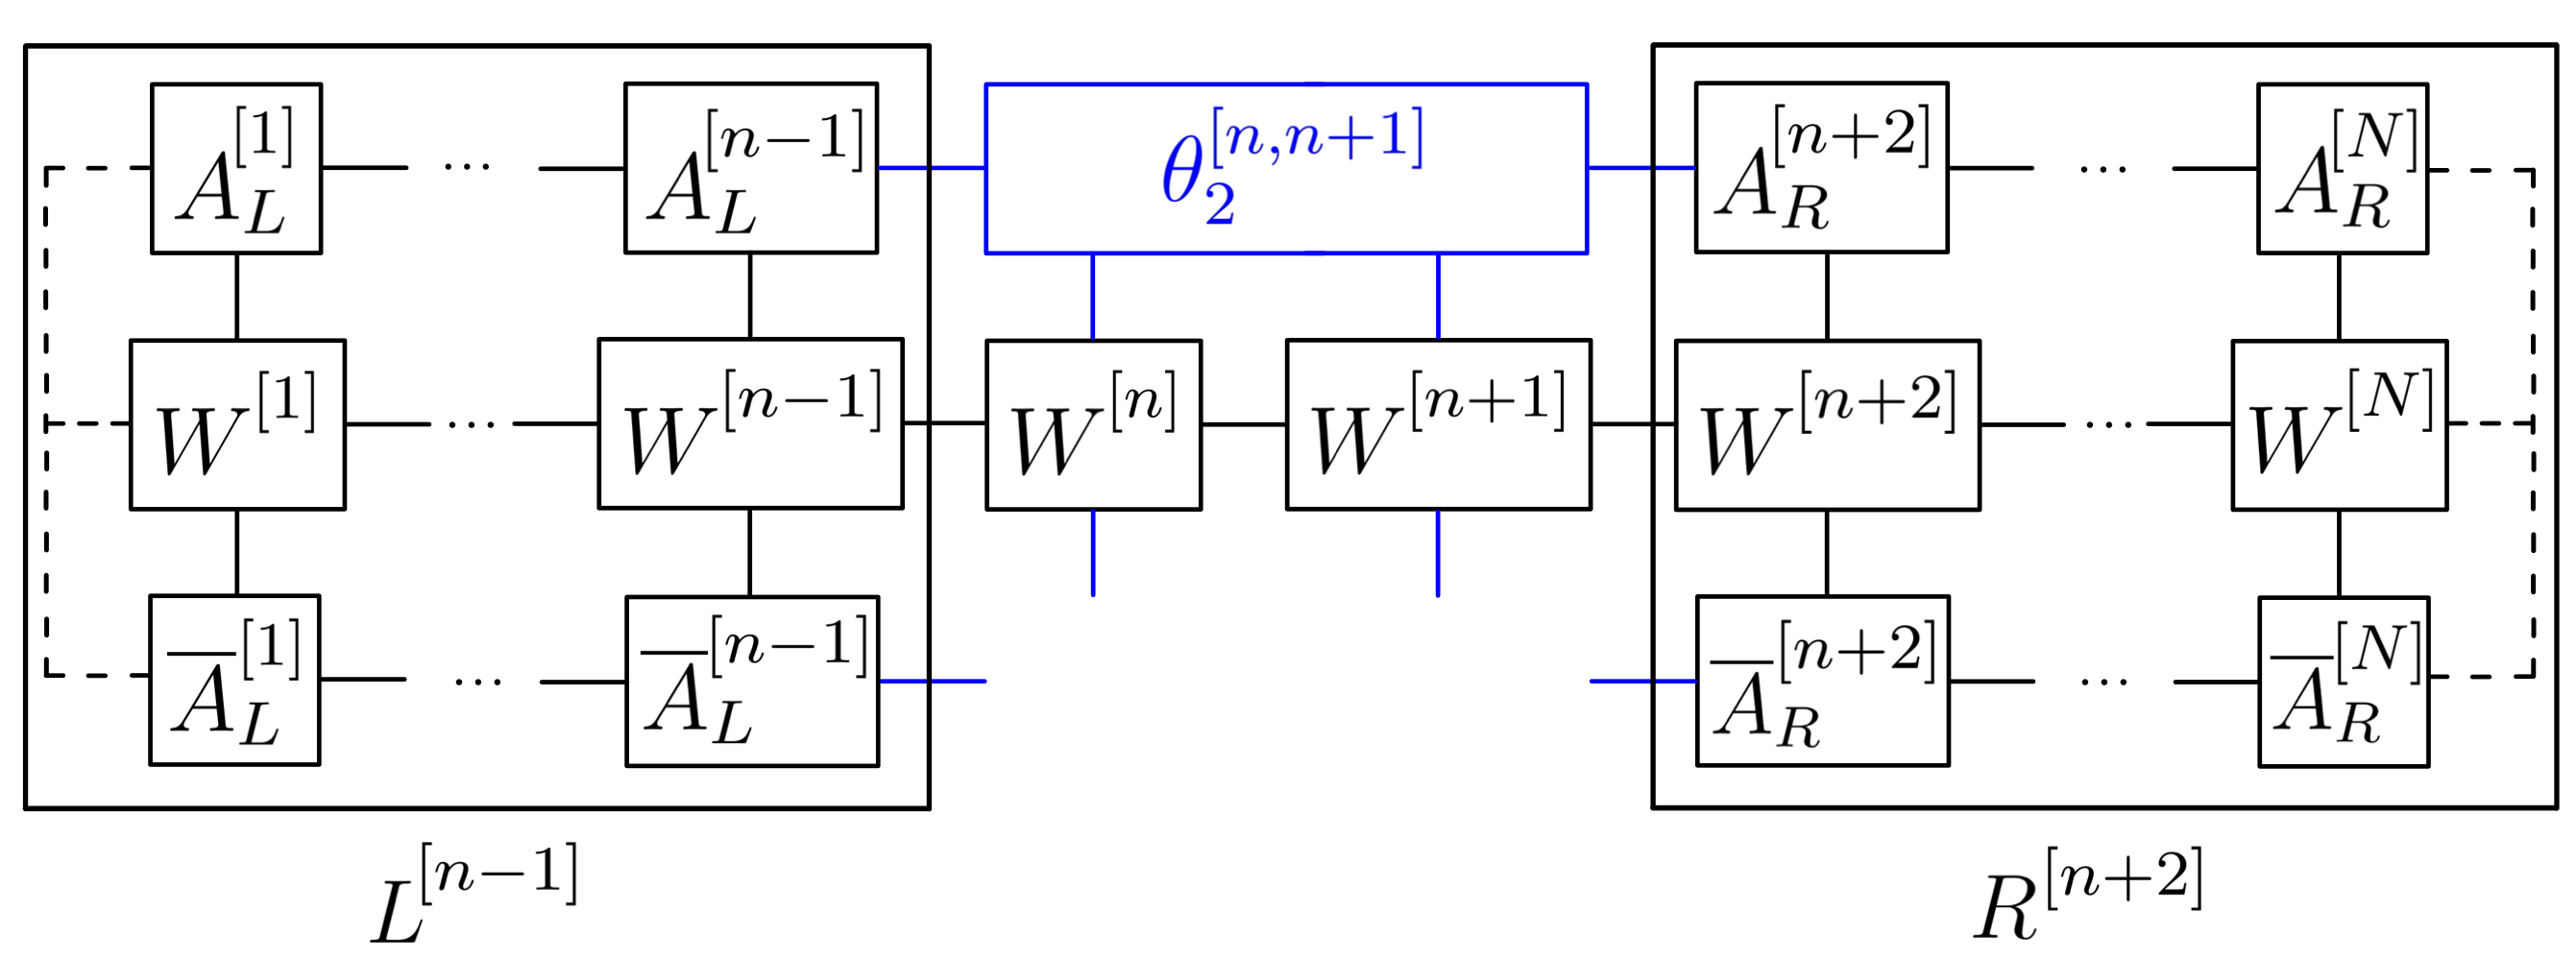
\includegraphics[height=4cm]{Heff2_theta2.png}} \hspace{0.2em}.
\end{equation}
We initialize the MPS with tensors $\{C^{[n]}\}_{n=0}^{N-1}$ and $\{A_R^{[n]}\}_{n=1}^{N}$. Since our two-site algorithm allows dynamical growth of entanglement, we can start from a product state, such as $\ket{\Rightarrow}$ with $C^{[n]} = ((1)) \in \mathbb{C}^{1 \times 1}$ and $A_R^{[n] \uparrow} = A_R^{[n] \downarrow} = ((1/\sqrt{2})) \in \mathbb{C}^{1 \times 1}$. To not compute recurrent parts of the network over and over again, it is good practice to store partial contractions as environment tenors $L^{[n]}$ and $R^{[n]}$. We initialize $L^{[0]} = R^{[N+1]} = (((1))) \in \mathbb{C}^{1 \times 1 \times 1}$ and compute $R^{[n]}$ for all $n = N, \ldots 3$ from $\{A_R^{[n]}\}_{n=N}^{3}$ and $\{W^{[n]}\}_{n=N}^{3}$. Then we sweep through the chain from left to right ($n = 1, \ldots, N-1$) and back from right to left ($n = N-2, \ldots, 1$) while performing the following updates:
\begin{enumerate}[leftmargin=4em]
	\item[A1)] With the current $\theta_2^{[n, n+1]} = C^{[n-1]} A_R^{[n]} A_R^{[n+1]}$ as initial guess, compute the ground state $\Tilde{\theta}_2^{[n, n+1]}$ of $H_{\mathrm{eff}, 2}^{[n, n+1]}$ using an iterative Lanczos method.
	\item[A2)] Split and truncate $\Tilde{\theta}_2^{[n, n+1]}$ by performing an SVD. Keep only singular values larger than $\epsilon$ and maximally $D_{\text{max}}$ of them:
\begin{equation}
	\raisebox{-0.5\height}{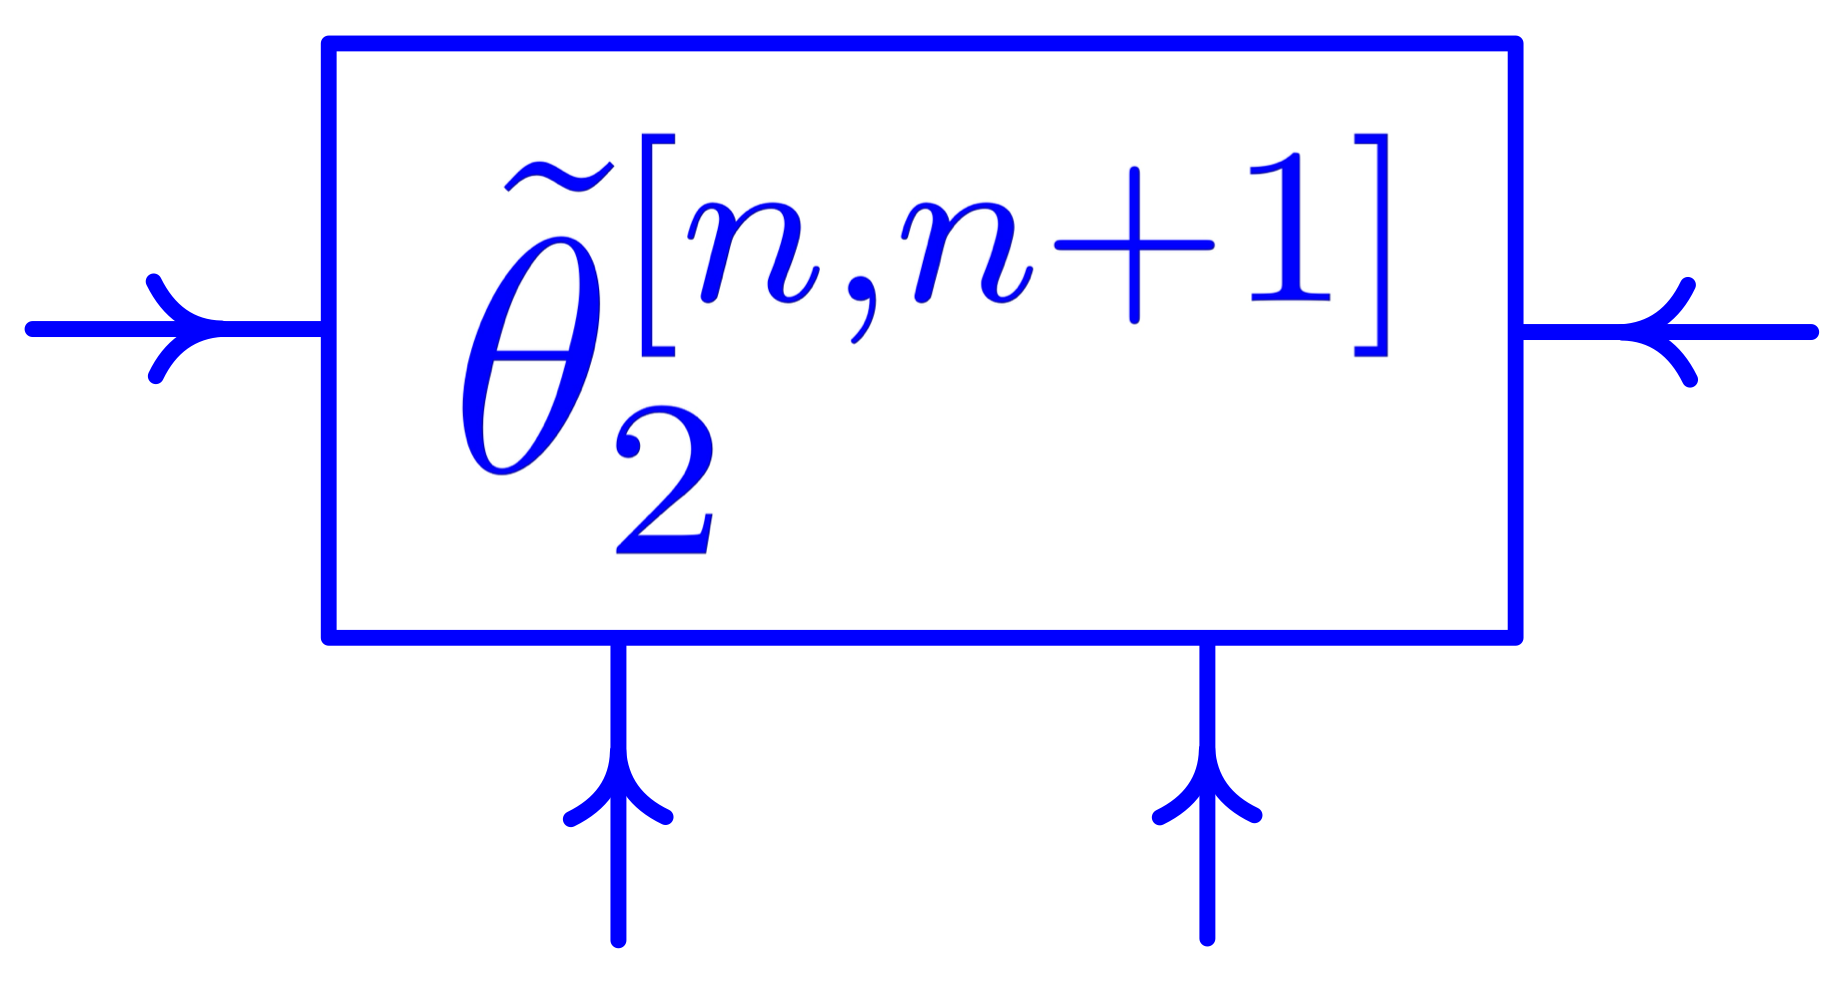
\includegraphics[height=1.3cm]{theta2_new.png}}
	\hspace{0.2em} \overset{\mathrm{\textcolor{red}{t}SVD}}{\rightarrow} \hspace{0.2em}
	\overset{\textcolor{red}{\mathrm{min}\left( \# \{ \Tilde{C}^{[n]}_{\alpha} > \epsilon\}, \: D_{\mathrm{max}} \right)}}{\raisebox{-0.5\height}{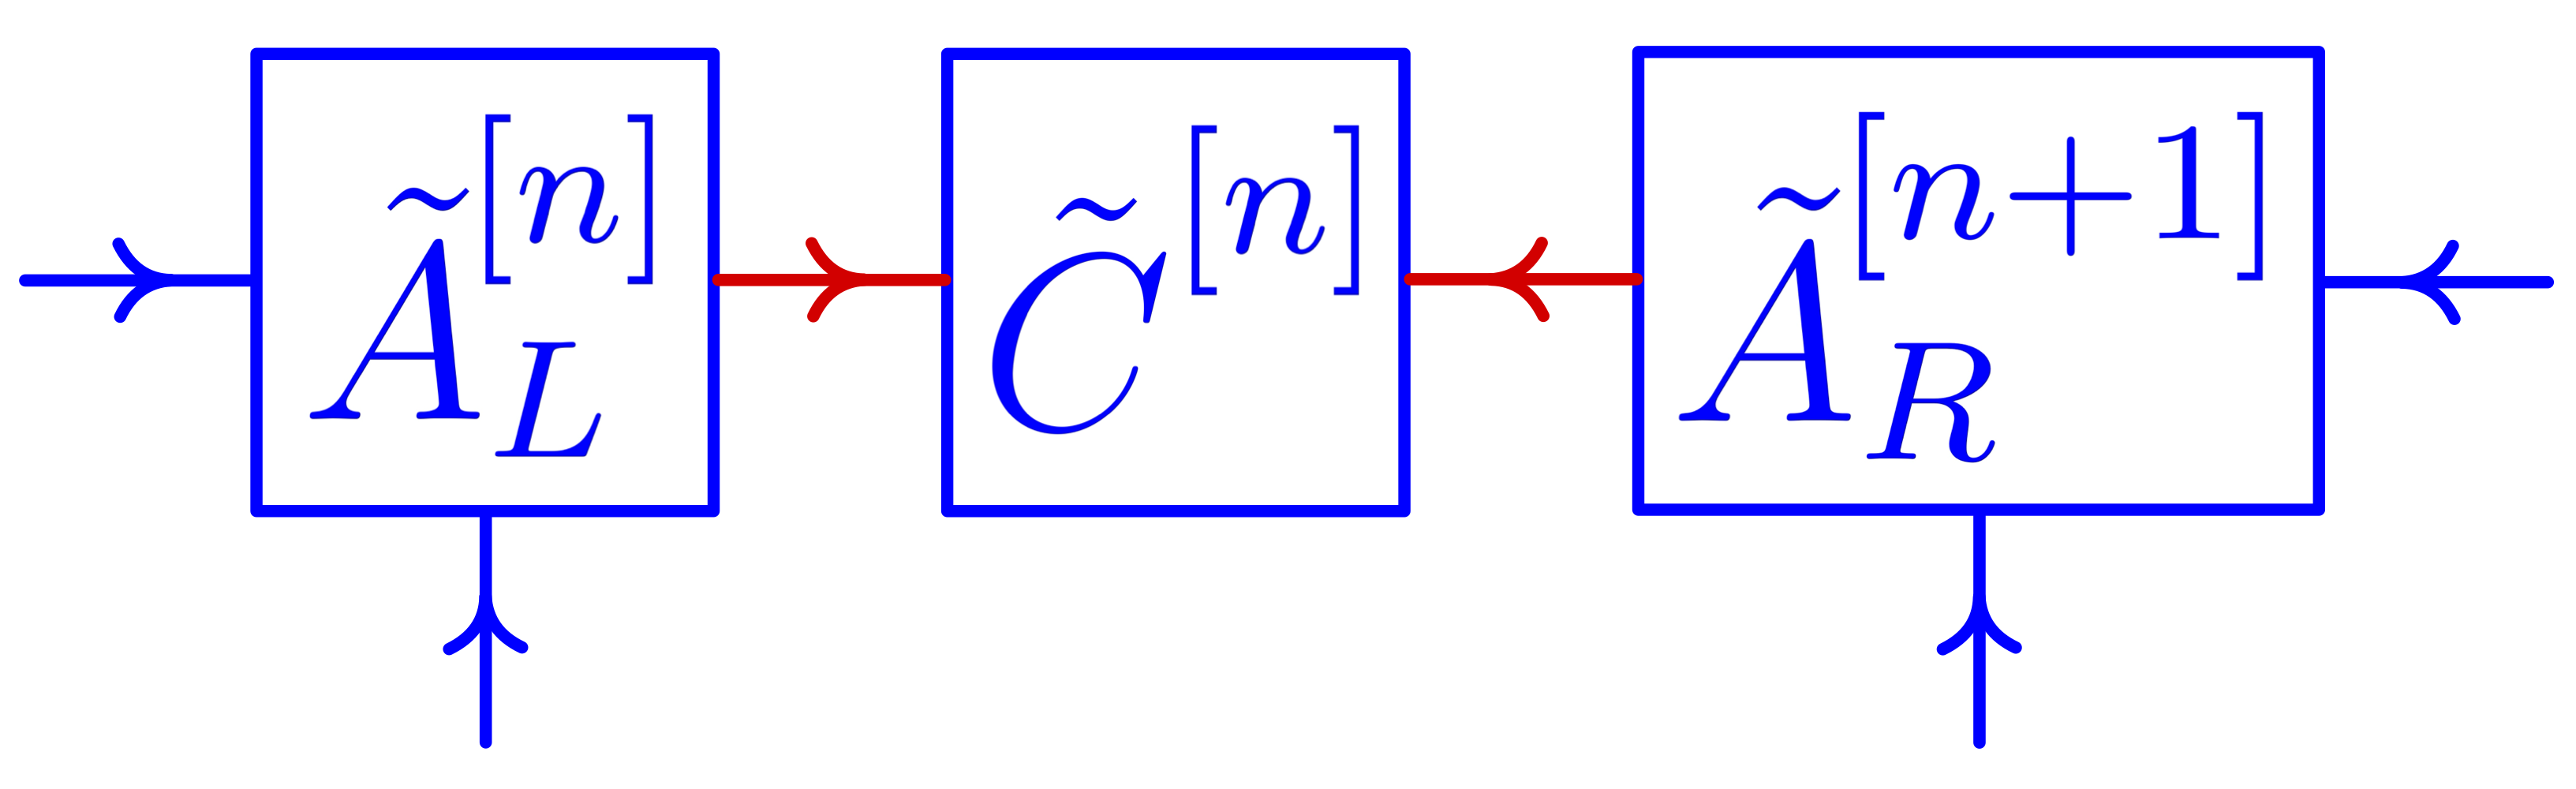
\includegraphics[height=1.3cm]{theta2_new_tsvd.png}}} \hspace{0.2em}.
\end{equation}
From this update the MPS according to:
\begin{equation} \label{eq:dmrg_mps_update}
A_R^{[n]} \rightarrow {(C^{[n-1]})}^{-1} \Tilde{A}_L^{[n]} \Tilde{C}^{[n]}	
\footnote{In general one should avoid inverting small singular values. In this case the inversion in $\Tilde{A}_R^{[n]} = {(C^{[n-1]})}^{-1} \Tilde{A}_L^{[n]} \Tilde{C}^{[n]}$ is effectively undone after computing $\Tilde{\theta}_2^{[n, n+1]} = C^{[n-1]} \Tilde{A}_R^{[n]} \Tilde{A}_R^{[n+1]}$ at a later point.}, \hspace{0.5em}
C^{[n]} \rightarrow \Tilde{C}^{[n]}, \hspace{0.5em}
A_R^{[n+1]} \rightarrow \Tilde{A}_R^{[n+1]}.
\end{equation}
	\item[A3)] Update the environments $L^{[n]}$ and $R^{[n+1]}$ using $\Tilde{A}_L^{[n]}$ and $\Tilde{A}_R^{[n+1]}$ respectively and move to the next site.
\end{enumerate}

% benchmark
\newpage
\noindent \underline{Benchmark} \\[0.5em]
For the TFI Hamiltonian \eqref{eq:mpo_pbc} with PBC and $N = 20$, we run $10$ of the just described DMRG sweeps with a singular value cutoff $\epsilon = 10^{-14}$. Of the final ground state approximation, we compute the translation expectation value
\begin{equation}
	\bra{\psi ( \overline{A} )}T \ket{\psi ( A )} =
	\raisebox{-0.5\height}{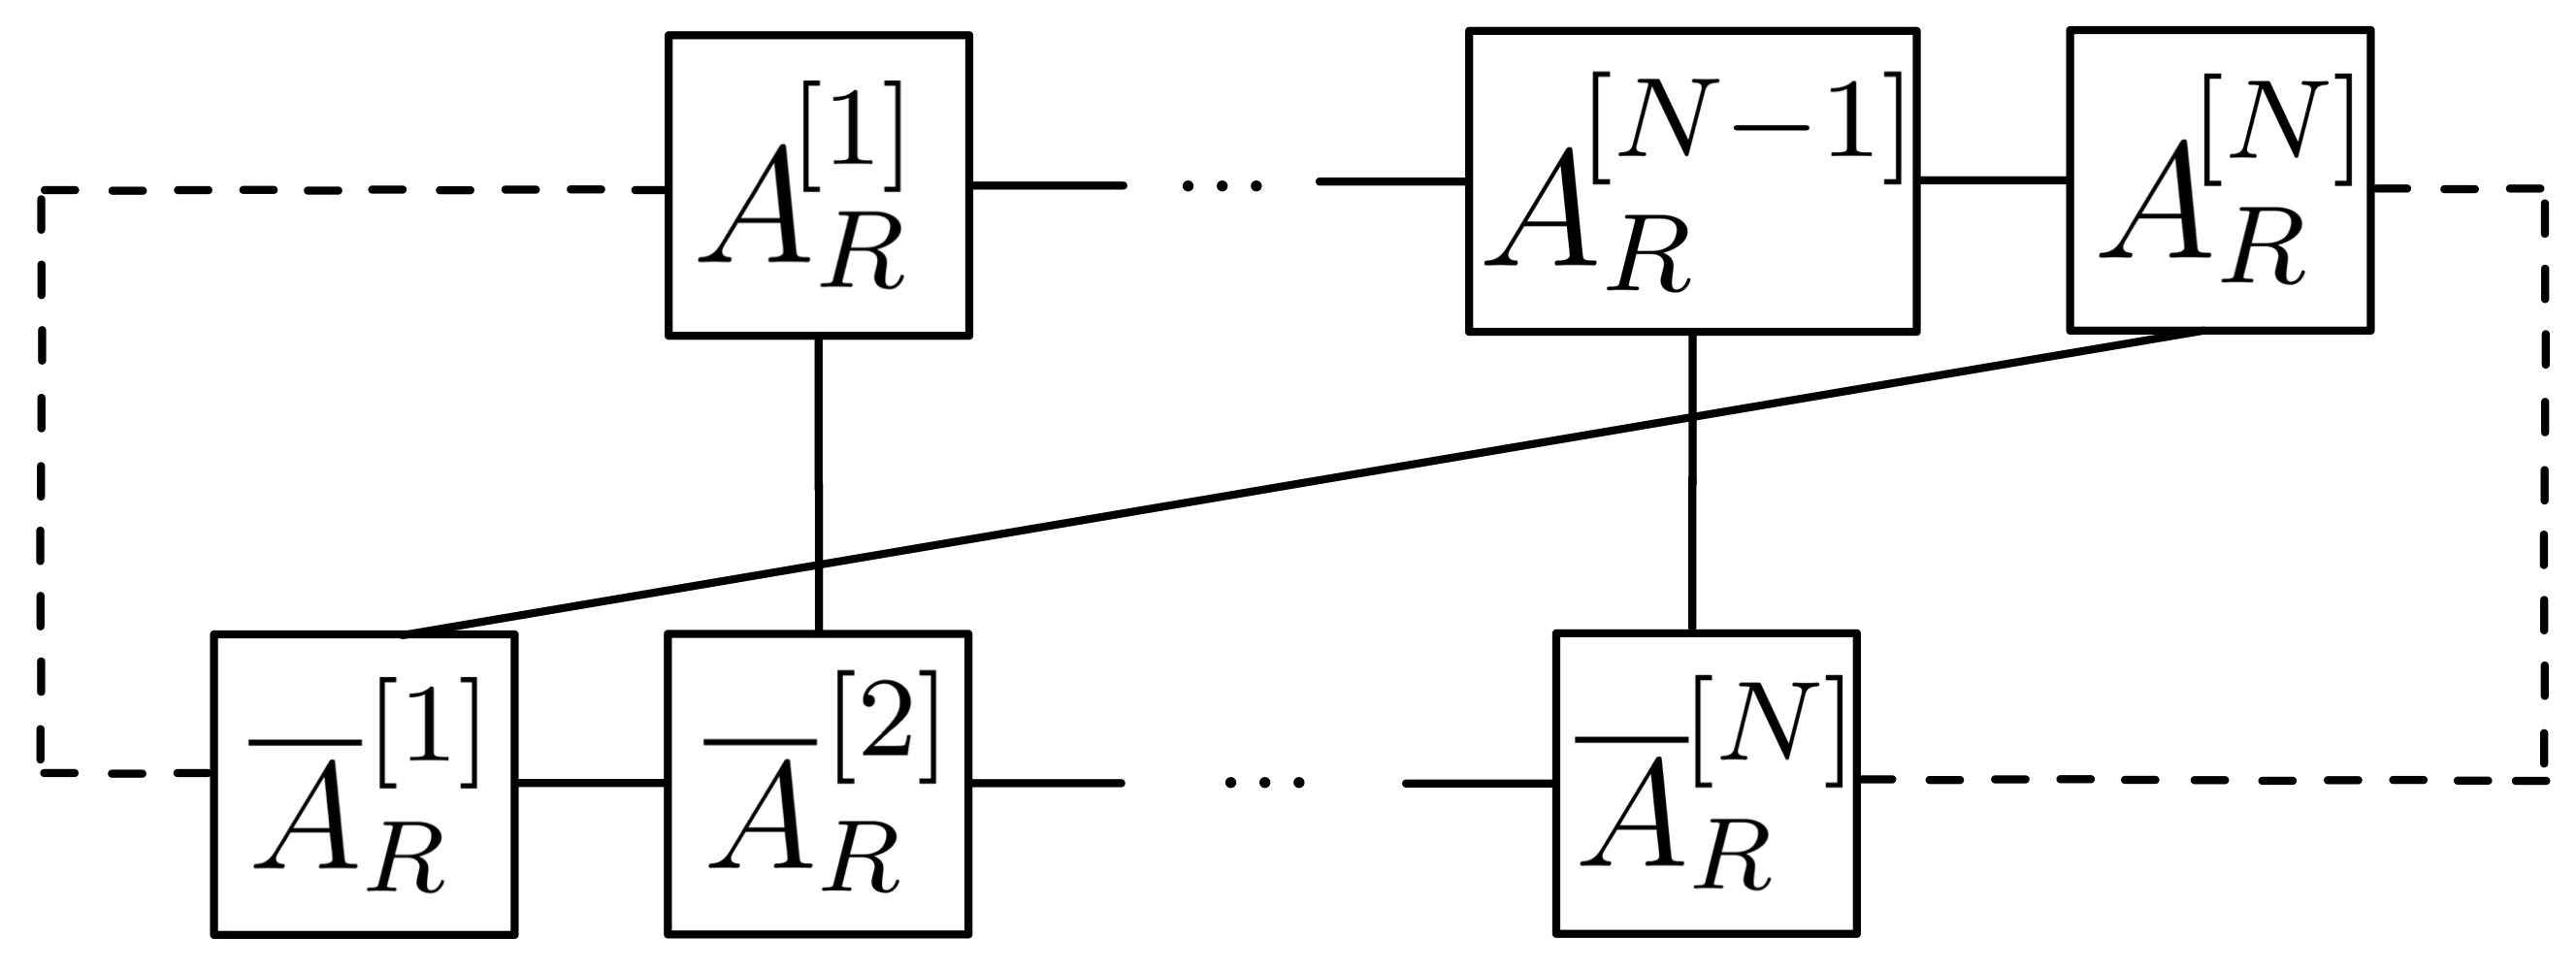
\includegraphics[height=2.5cm]{translation_ground_state.png}} \hspace{0.2em},
\end{equation}
its variance, and the variance of the Hamiltonian. In the left panels (a) of figure \ref{fig:dmrg} we plot the results against the maximal bond dimension $D_{\text{max}}$. Even though the MPS has OBC, the variances of the PBC Hamiltonian and the translation operator fall below $10^{-10}$ for $D_{\text{max}} \gtrsim 64$. This restores momentum as a good quantum number, with a value zero for the ground state.
\begin{figure}[t]
  \centering
  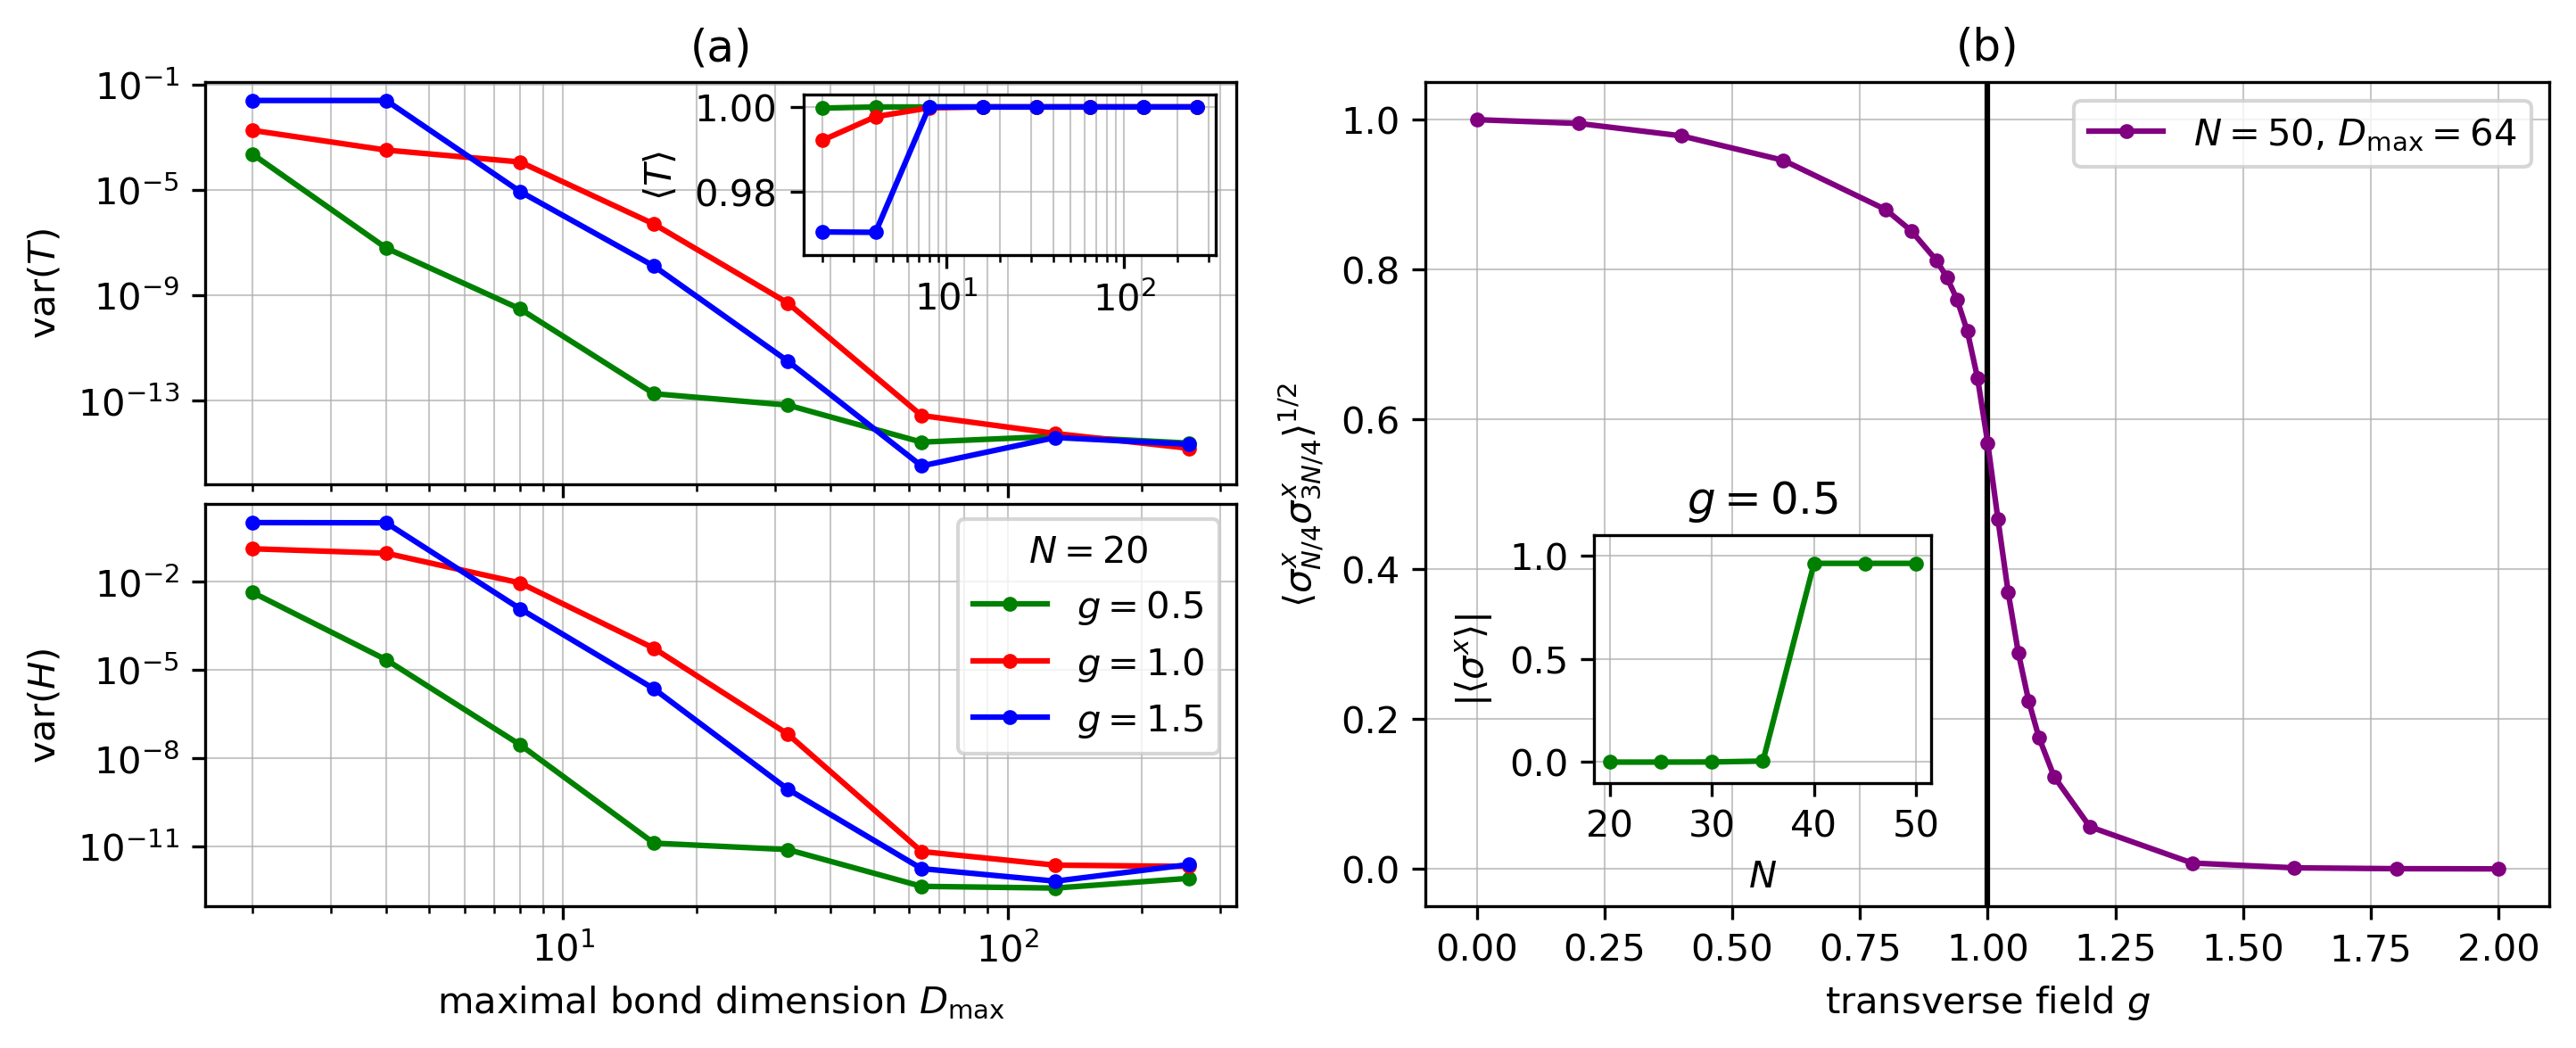
\includegraphics[width=1.0\linewidth]{dmrg.png}
  \caption{TFI benchmark for the DMRG algorithm with periodic Hamiltonian. For the left plots (a), we take a chain of length $N = 20$ and perform $10$ DMRG ground state sweeps with a singular value cutoff $\epsilon = 10^{-14}$ and various maximal bond dimensions $D_{\text{max}}$. Even though the MPS has OBC, the variances of the PBC Hamiltonian and the translation operator fall below $10^{-10}$ for $D_{\text{max}} \gtrsim 64$. This restores momentum as a good quantum number, with value zero for the ground state (concluded from the inset plot that converges to $\langle T \rangle = 1$). In the inset of the right panel (b), we show that for system sizes $N \lesssim 35$ (at $g = 0.5$), DMRG is able to resolve the exponentially small energy splitting $\delta E_{\pm} = \mathcal{O}(g^N)$ between the symmetric superpositions $\frac{1}{\sqrt{2}}(\ket{\Rightarrow} \pm \ket{\Leftarrow})$. For $N=50$, we plot the magnetization order parameter $m = \langle \sigma^x_{N/4} \sigma^x_{3N/4} \rangle^{1/2}$ against $g$. Compared to the sharp transition in the infinite case, $m$ goes to zero smoothly around $g = 1$.}
\label{fig:dmrg}
\end{figure}

% VQPE
\newpage
\section{Variational quasiparticle excitations (VQPE)} \label{sec:vqpe}
Completely analogous to the uniform case \eqref{eq:uexcitation_ansatz}, but without the explicit momentum phase, we create a quasiparticle excitation above an MPS ground state $\ket{\psi(A)}$ by inserting local tensor perturbations $\{B^{[n]} \in \mathbb{C}^{D_{n-1} \times d \times D_n}\}_{n=1}^N$ for the center tensors $\{A_C^{[n]}\}_{n=1}^N$ in canonical form \cite{van2021efficient}:
\begin{equation} \label{eq:excitation_ansatz}
	\ket{\psi(B; A)} = \sum_{n=1}^N \raisebox{-0.55\height}{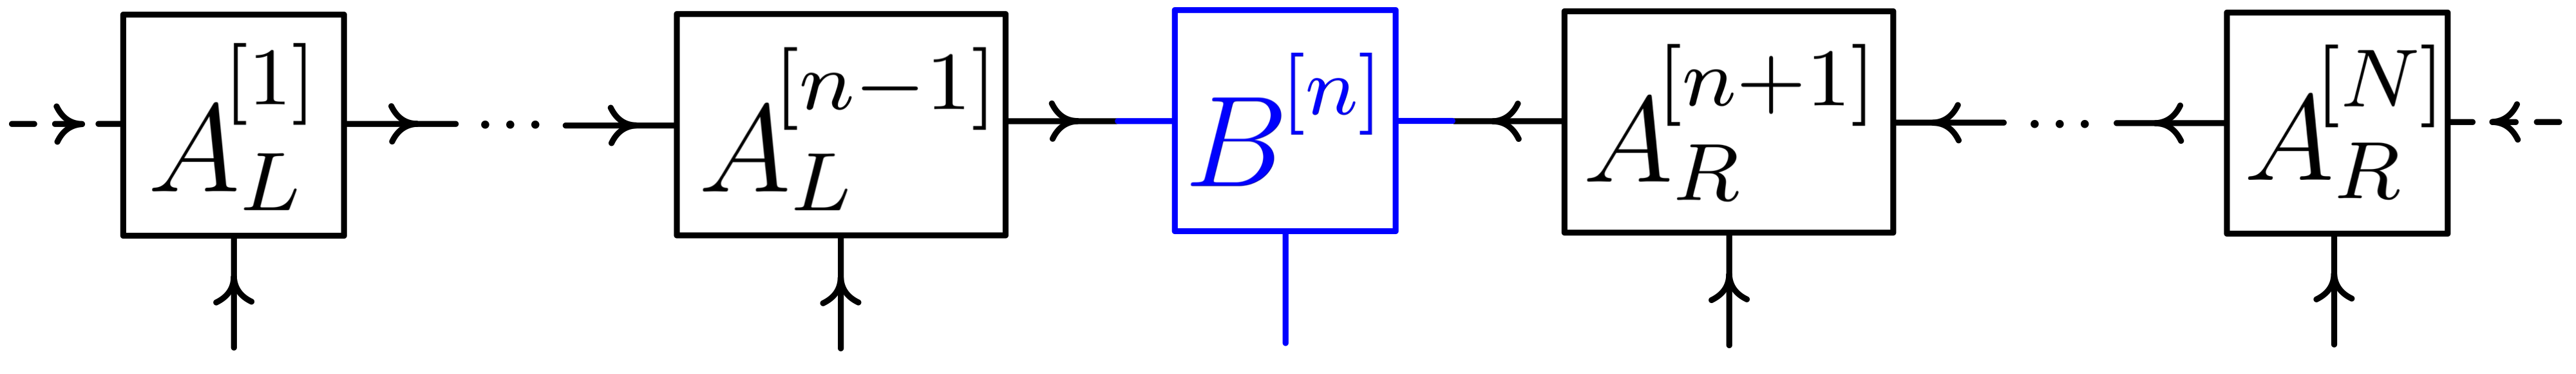
\includegraphics[height=1.25cm]{emps.png}} \hspace{0.2em}.
\end{equation}
This can be interpreted as a tangent space vector, by applying the definition \eqref{eq:tangent_space_vector_mps} to the left isometric tensors $\{A_L^{[n]}\}_{n=1}^N$ and then, for each term in the sum, moving the full rank center matrix from the very right to the perturbation tensor and absorbing it therein. \\[1em]

% gauge fixing
\noindent \underline{Gauge fixing} \\[0.5em]
\noindent For any set of matrices $\{Y^{[n]} \in \mathbb{C}^{D_n \times D_n}\}_{n=1}^N$, the state \eqref{eq:excitation_ansatz} does not change under the additive gauge transformation
\begin{equation} 
	B^{[n]} \rightarrow B^{[n]} + A_L^{[n]} Y^{[n]} - Y^{[n-1]} A_R^{[n]} \text{ with } Y^{[0]} = Y^{[N]} \in \mathbb{C}.
\end{equation}
We fix the $\sum_{n=1}^N D_n^2$ gauge parameters by setting $B^{[n]} = 0$ if $D_{n-1} d = D_n$ and
\begin{equation} \label{eq:excitation_gauge}
	\text{if } D_{n-1} d > D_n: \hspace{0.5em}
	\raisebox{-0.55\height}{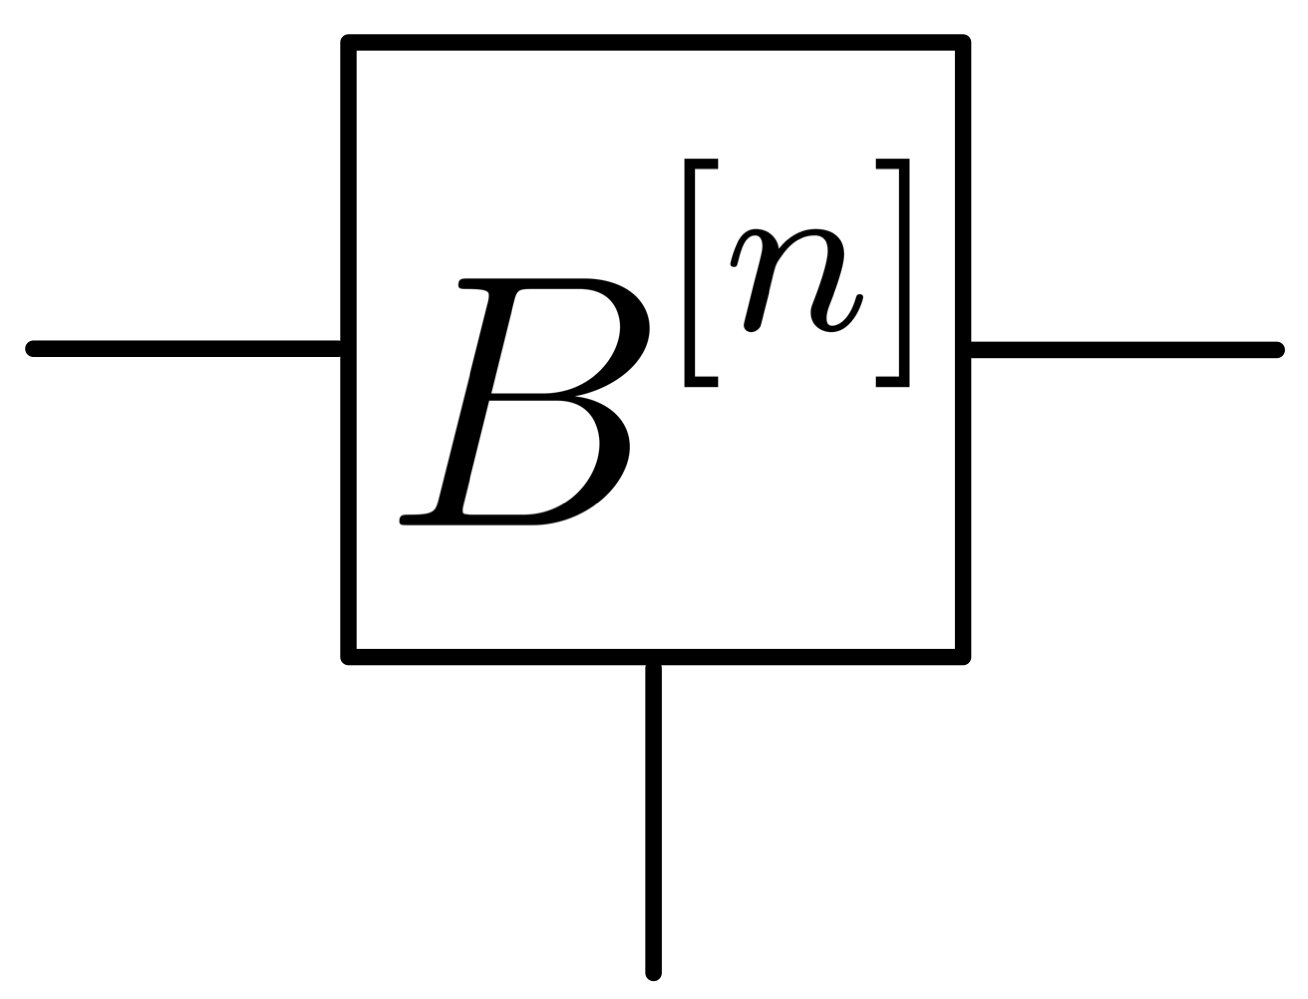
\includegraphics[height=1.2cm]{B.png}} 
	\:=\: 
	\raisebox{-0.45\height}{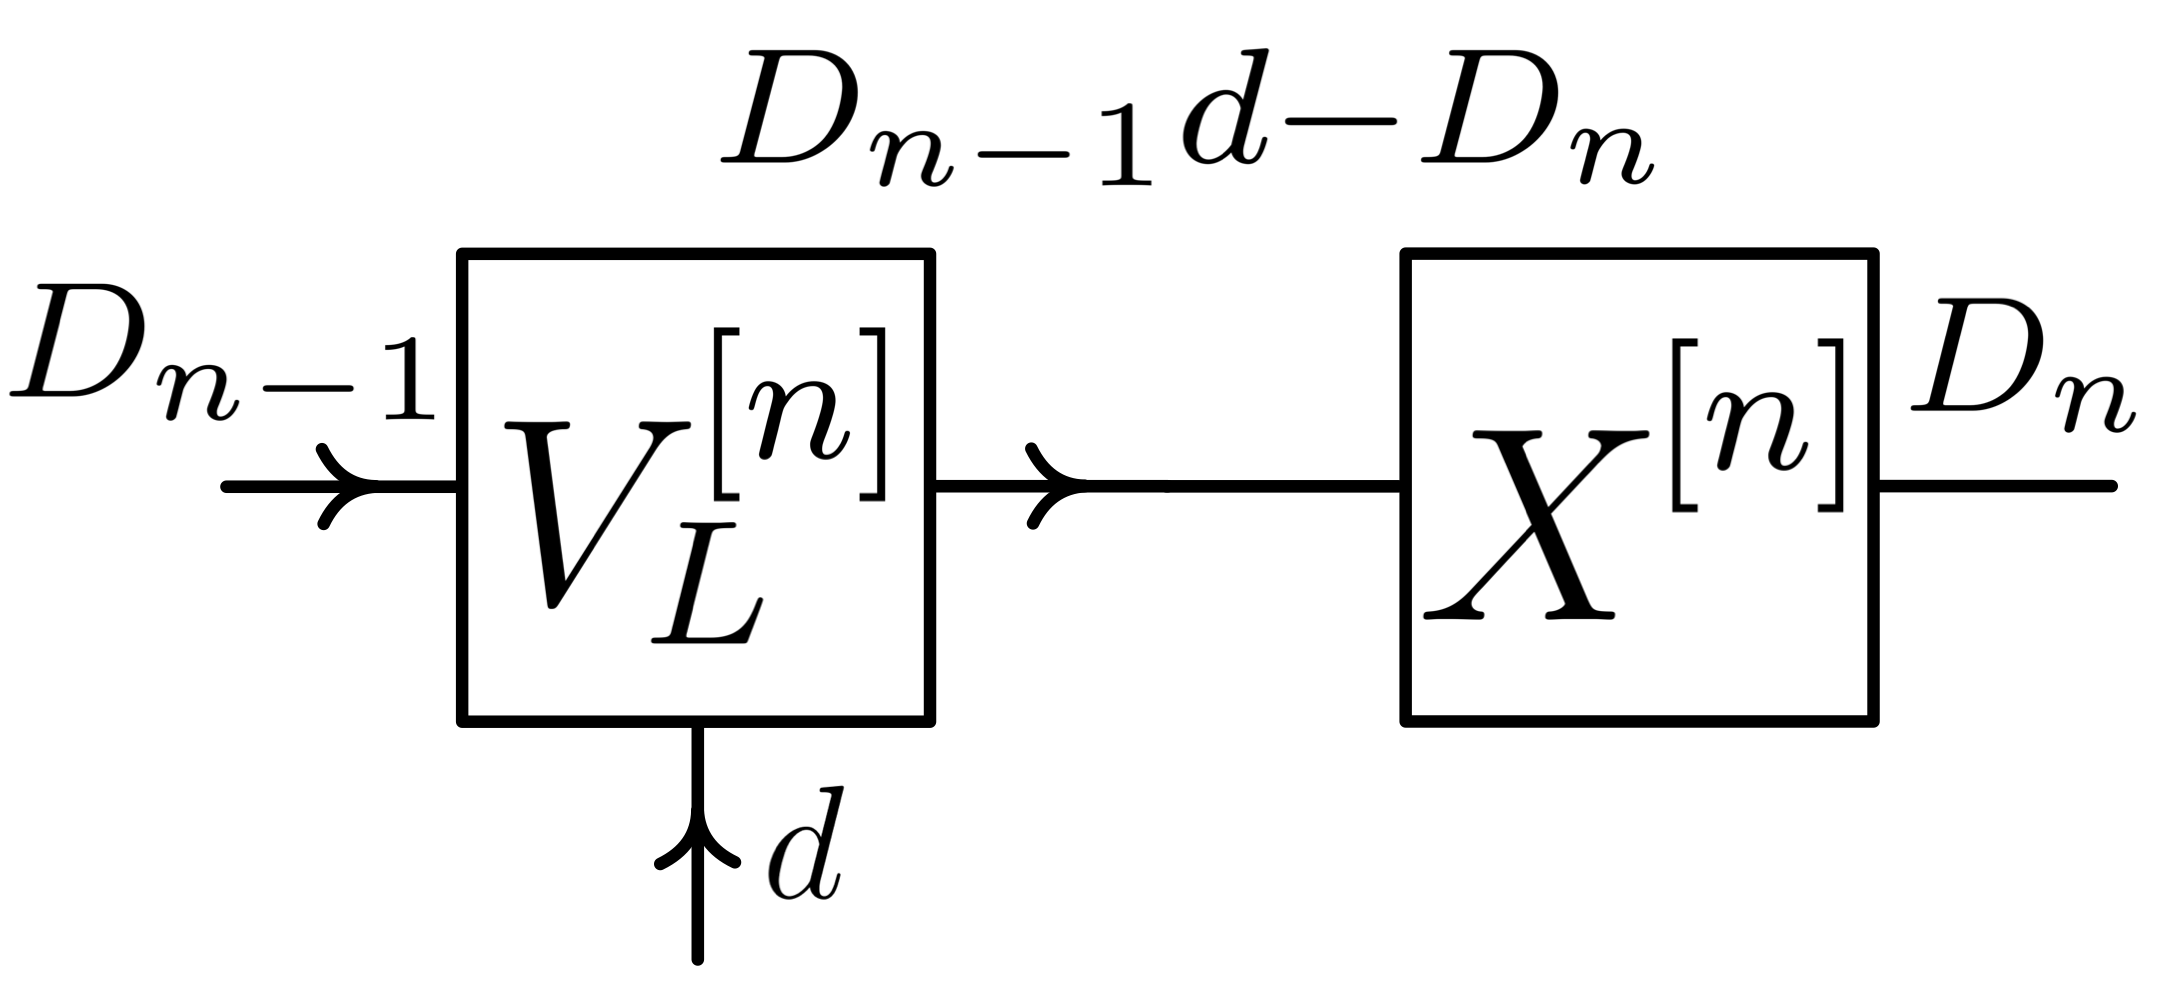
\includegraphics[height=1.6cm]{VL_X.png}} 
	\:\:\text{ with }\:\: 
	\raisebox{-0.45\height}{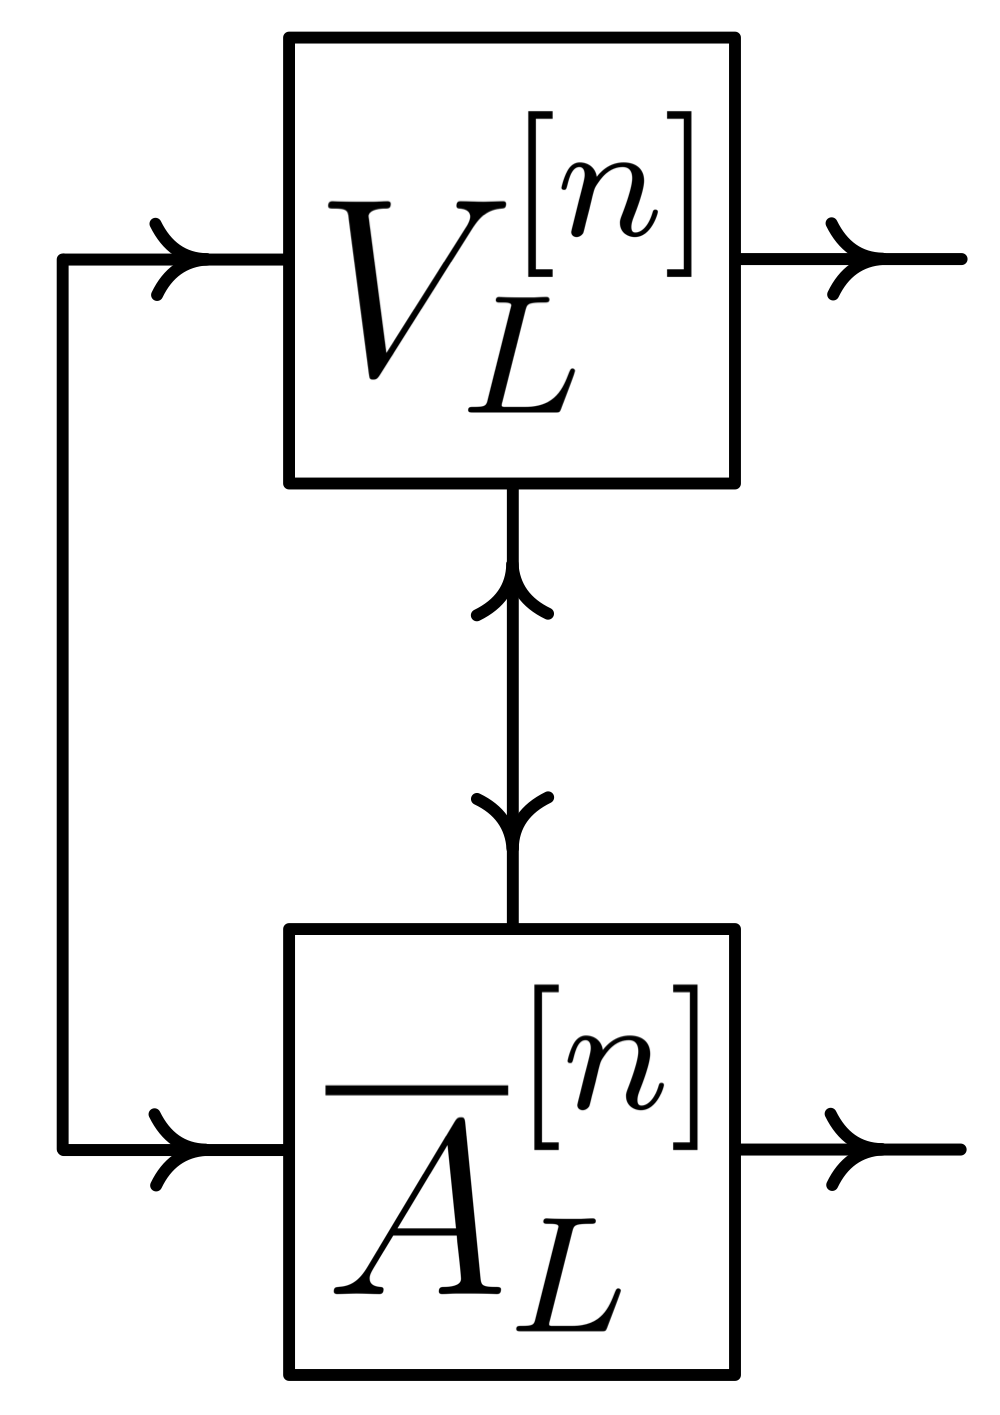
\includegraphics[height=2.35cm]{VL_AL.png}} 
	= 0.
\end{equation}
This ensures that the individual states $\ket{\psi(X^{[n]}; A)}$ in the superposition
\begin{equation} \label{eq:emps_X}
	\ket{\psi(X; A)} = \sum_{n=1}^N \ket{\psi(X^{[n]}; A)} = \sum_{n=1}^N \raisebox{-0.5\height}{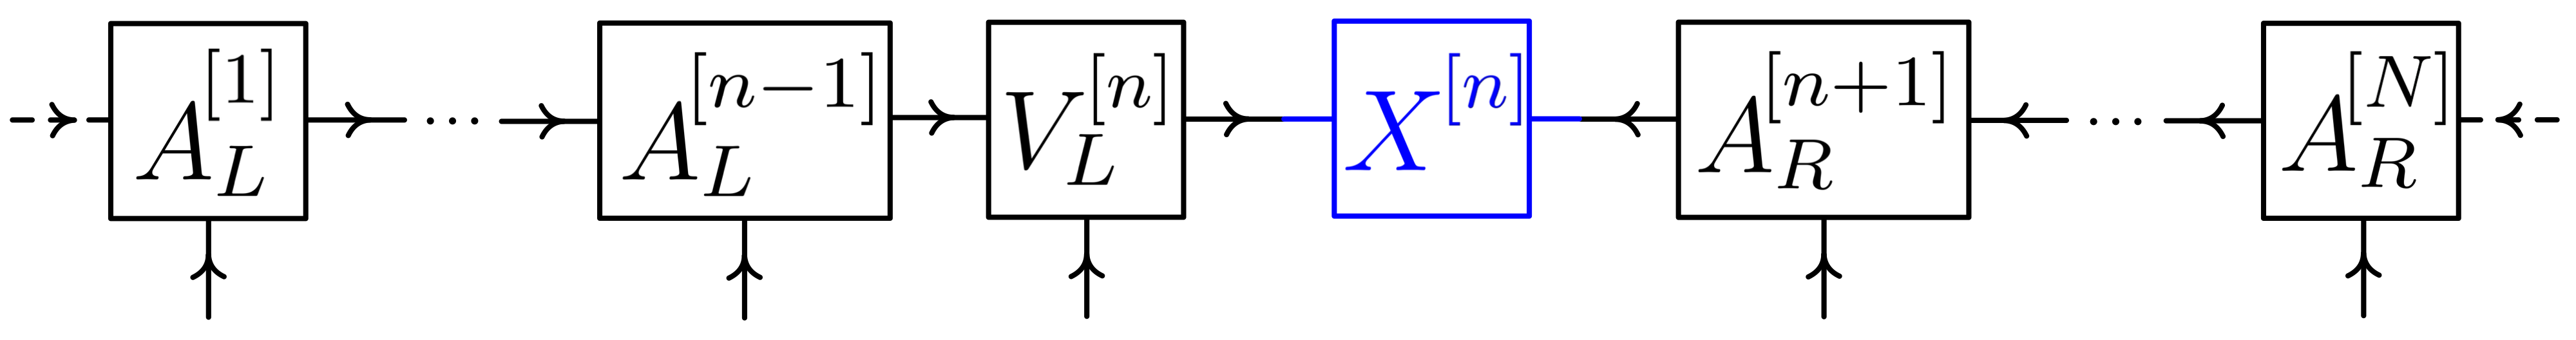
\includegraphics[height=1.3cm]{emps_X.png}}
\end{equation}
are orthogonal to the ground state and pairwise to each other:
\begin{equation} \label{eq:emps_orthogonality}
	\langle \psi(\overline{A}) \vert \psi(X^{[n]}; A) \rangle = 0, \hspace{0.5em}
	\langle \psi(\overline{Y}^{[m]}; \overline{A}) \vert \psi(X^{[n]}; A) \rangle = \delta_{nm} ( \overline{Y}^{[m]} \vert X^{[n]} ).
\end{equation}
From the latter relation it follows that the map $X \mapsto \ket{\psi(X; A)}$ is injective with 
\begin{equation} \label{eq:norm_excitation}
	\langle \psi(\overline{X}; \overline{A}) \vert \psi(X; A) \rangle = \sum_n ( \overline{X}^{[n]}  \vert X^{[n]} ). 
\end{equation}

% effective hamiltonian
\newpage
\begin{samepage}
\noindent \underline{Effective Hamiltonian} \\[0.5em]
\noindent Equation \eqref{eq:norm_excitation} further implies an identity norm matrix in the effective eigenvalue equation \eqref{eq:effective_eigenvalue_equation}. We solve it for $X^{[n]}$ by solving
\begin{equation} \label{eq:effective_excitation_equation}
	\partial_{\overline{B}^{[n]}} \tbra{\overline{B}} H_{\text{eff}} \tket{B} = \lambda \tket{B^{[n]}}
\end{equation} 
for $B^{[n]} = V_L^{[n]} X^{[n]}$.\footnote{We implement the effective matrix-vector multiplication by transforming $X \rightarrow B = \{V_L^{[n]}X^{[n]}\}$, computing $\tilde{B}^{[n]} = \partial_{\overline{B}^{[n]}} \tbra{\overline{B}} H_{\text{eff}} \tket{B}$, and transforming back to $\tilde{X} = \{\overline{V}_L^{[n]}\tilde{B}^{[n]}\}$.} For the action of the effective Hamiltonian,
\begin{equation*}
	\textcolor{blue}{\tbra{\overline{B}}} H_{\mathrm{eff}} \textcolor{blue}{\tket{B}} = \sum_{n=1}^N 
	\left[
	\raisebox{-0.47\height}{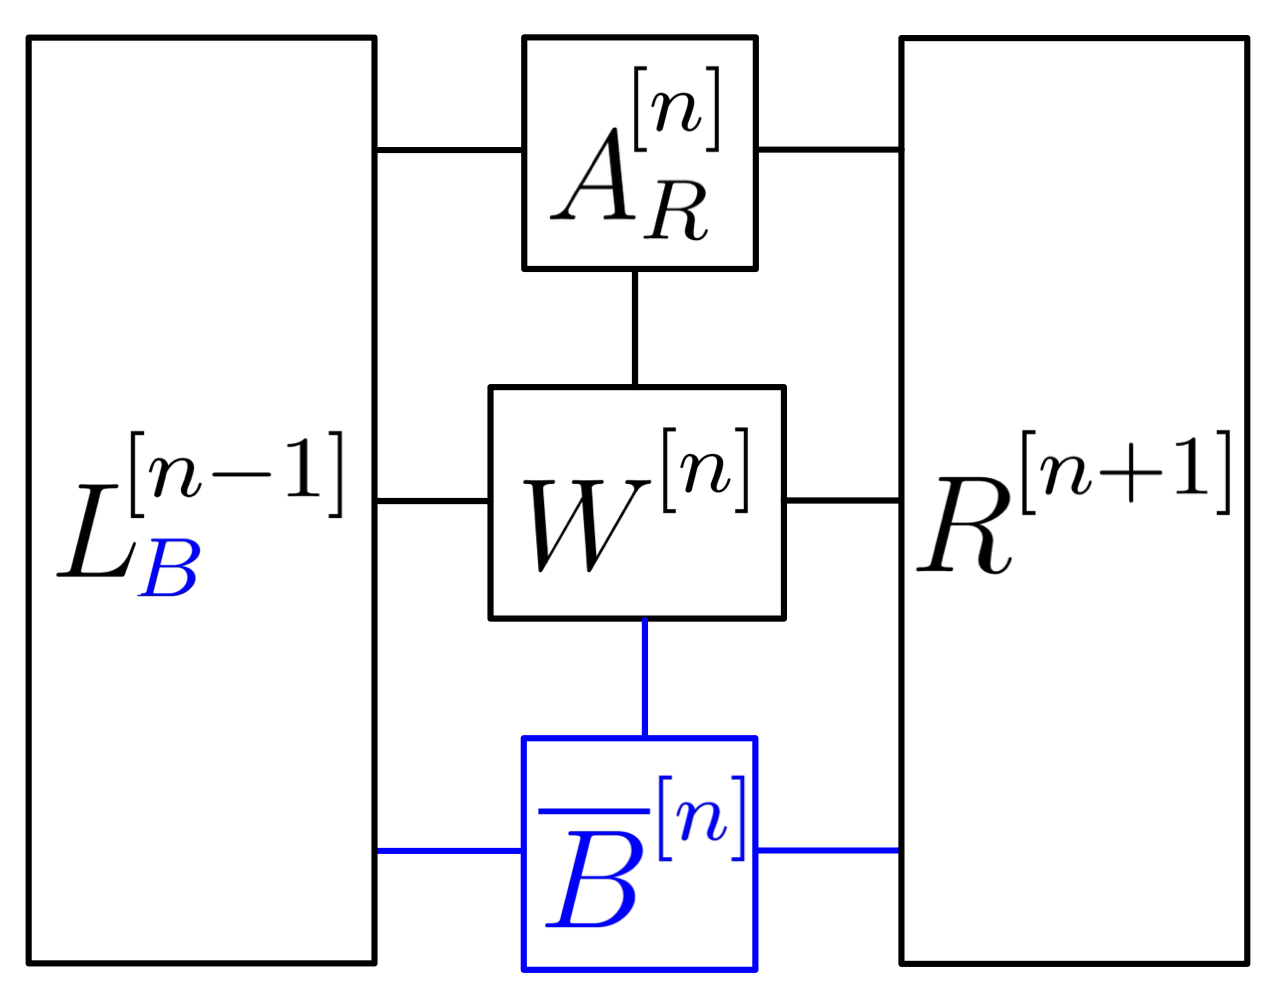
\includegraphics[height=3cm]{Heff1.png}}
	\:+\:
	\raisebox{-0.47\height}{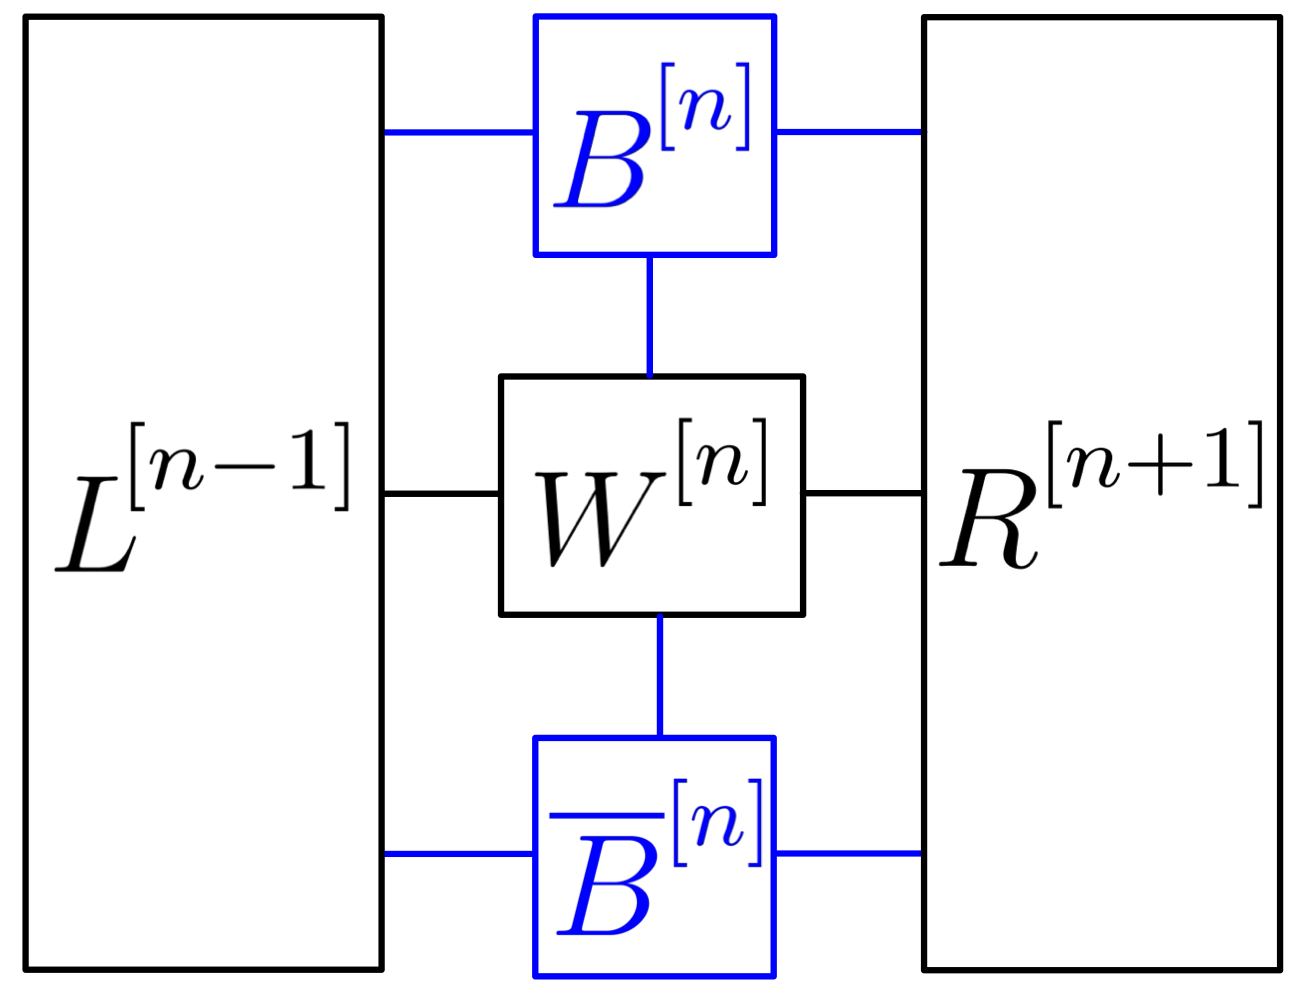
\includegraphics[height=3cm]{Heff2.png}}
	\:+\:
	\raisebox{-0.47\height}{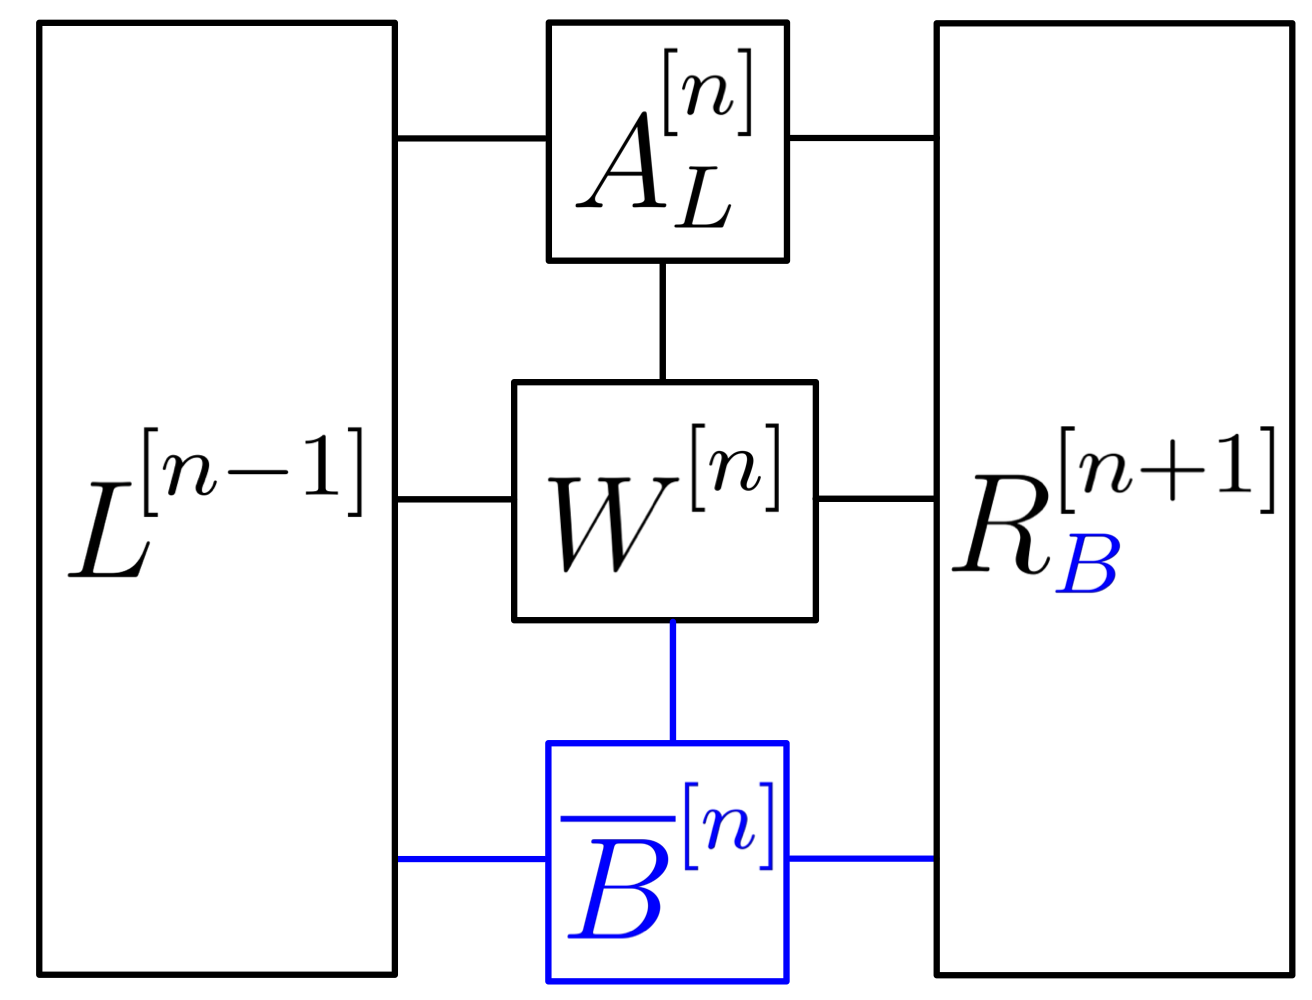
\includegraphics[height=3cm]{Heff3.png}}
	\right],
\end{equation*}
we compute the following boundary tensors iteratively starting from $L^{[0]} = R^{[N+1]} = (((1))) \in \mathbb{C}^{1 \times 1 \times 1}$ and $L_{\textcolor{blue}{B}}^{[0]} = R_{\textcolor{blue}{B}}^{[N+1]} = 0$:
\begin{equation} \label{eq:L_LB_R_RB}
\begin{array}{l c l}
	\raisebox{-0.5\height}{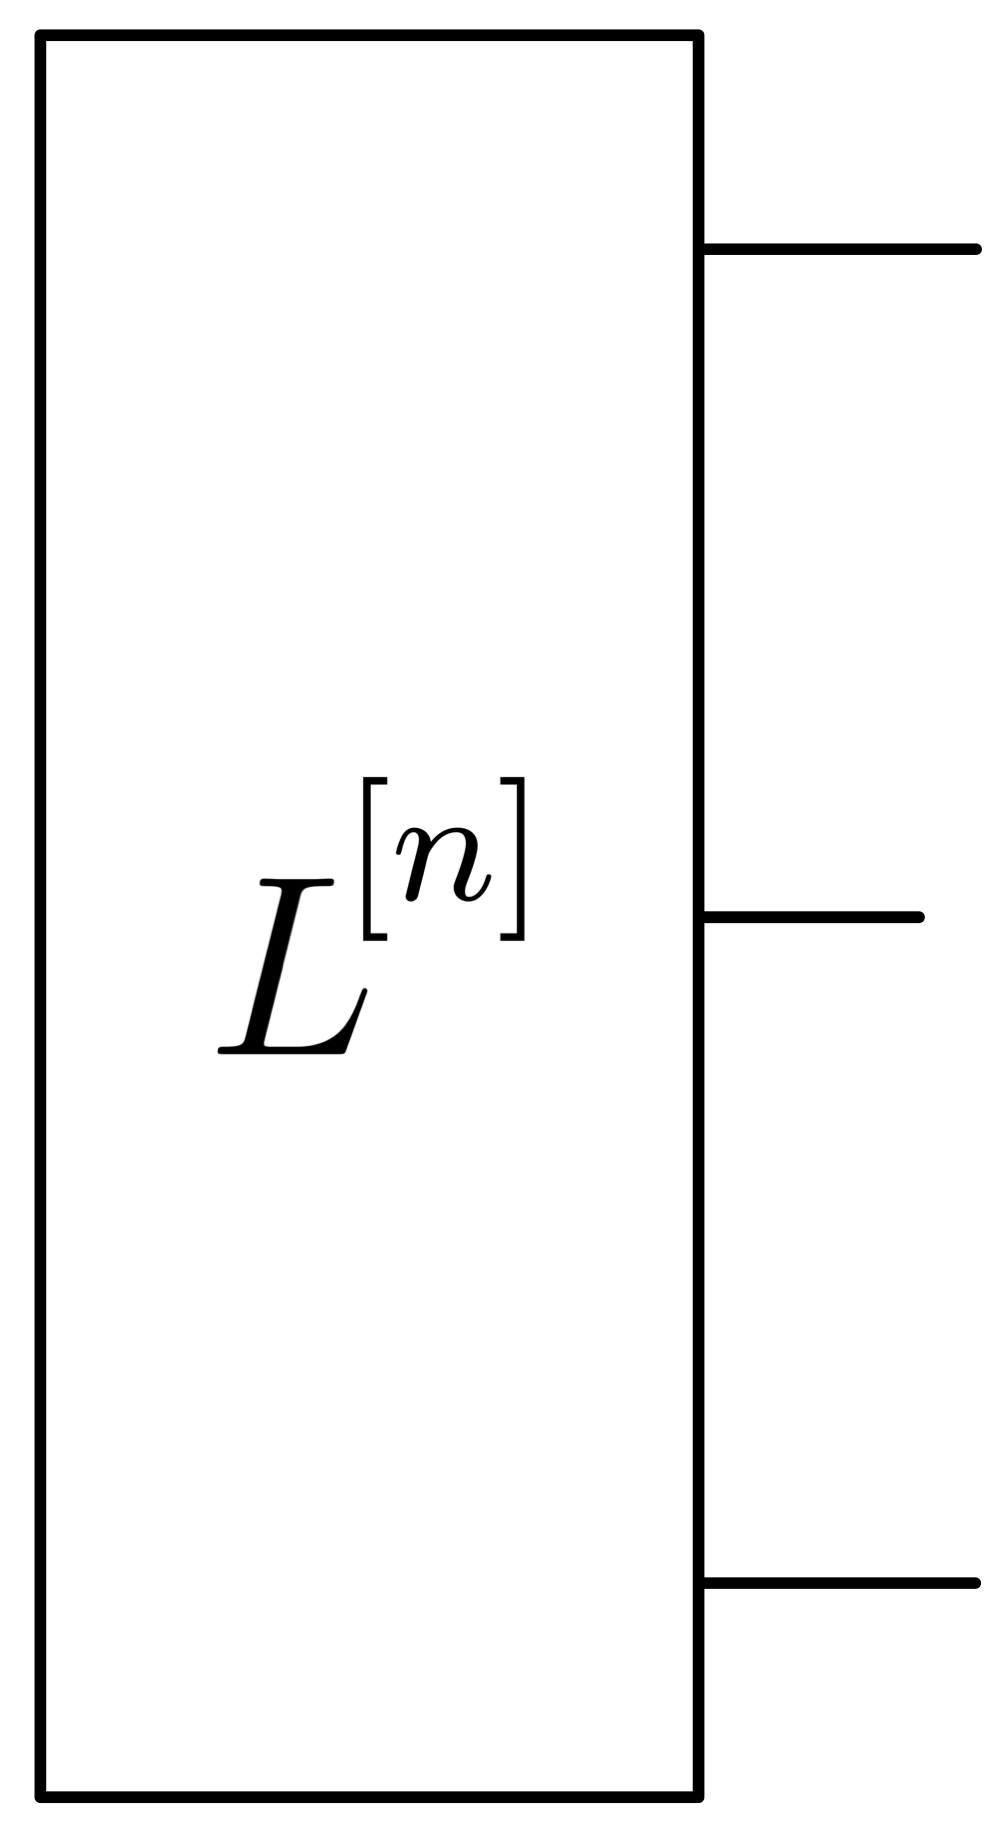
\includegraphics[height=3cm]{L1.png}} 
	\:=\:
	\raisebox{-0.5\height}{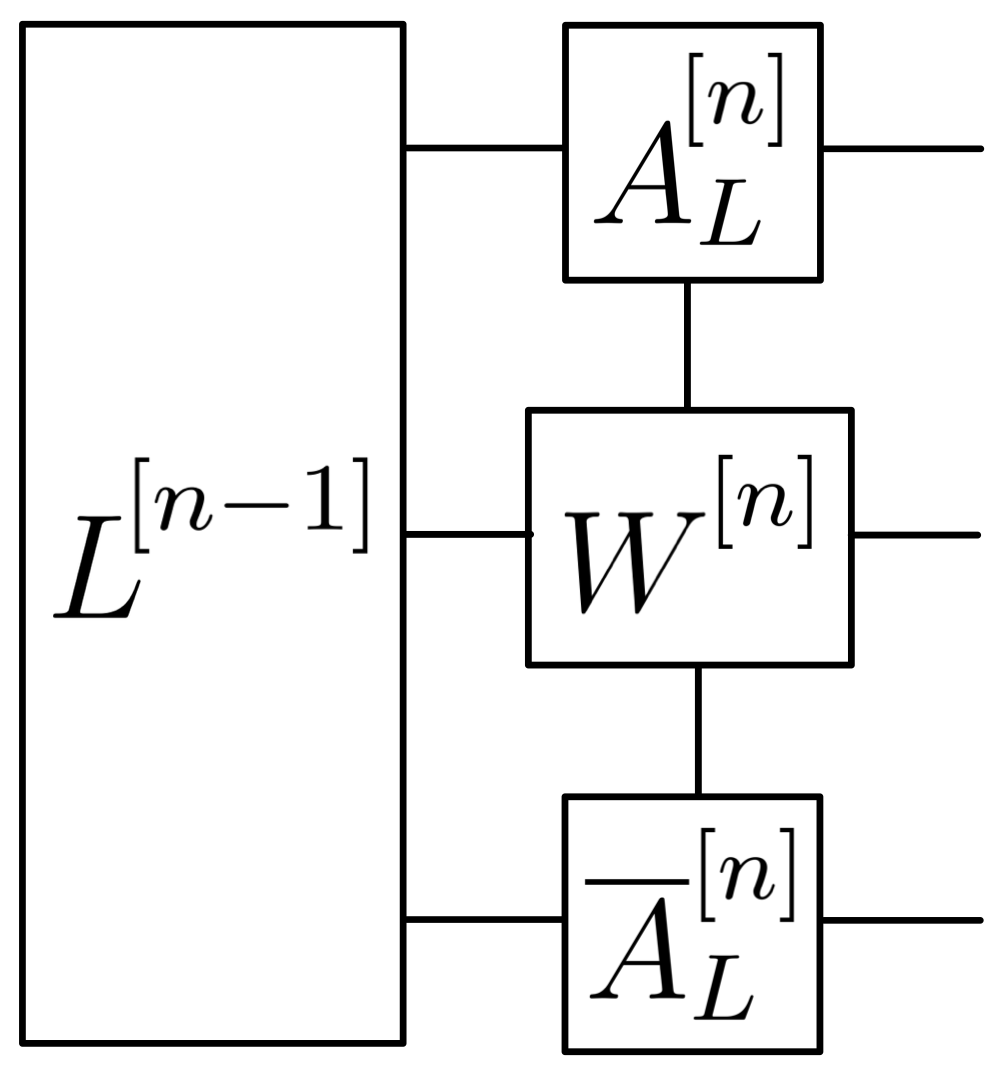
\includegraphics[height=3cm]{L2.png}} 
& ; &
	\raisebox{-0.5\height}{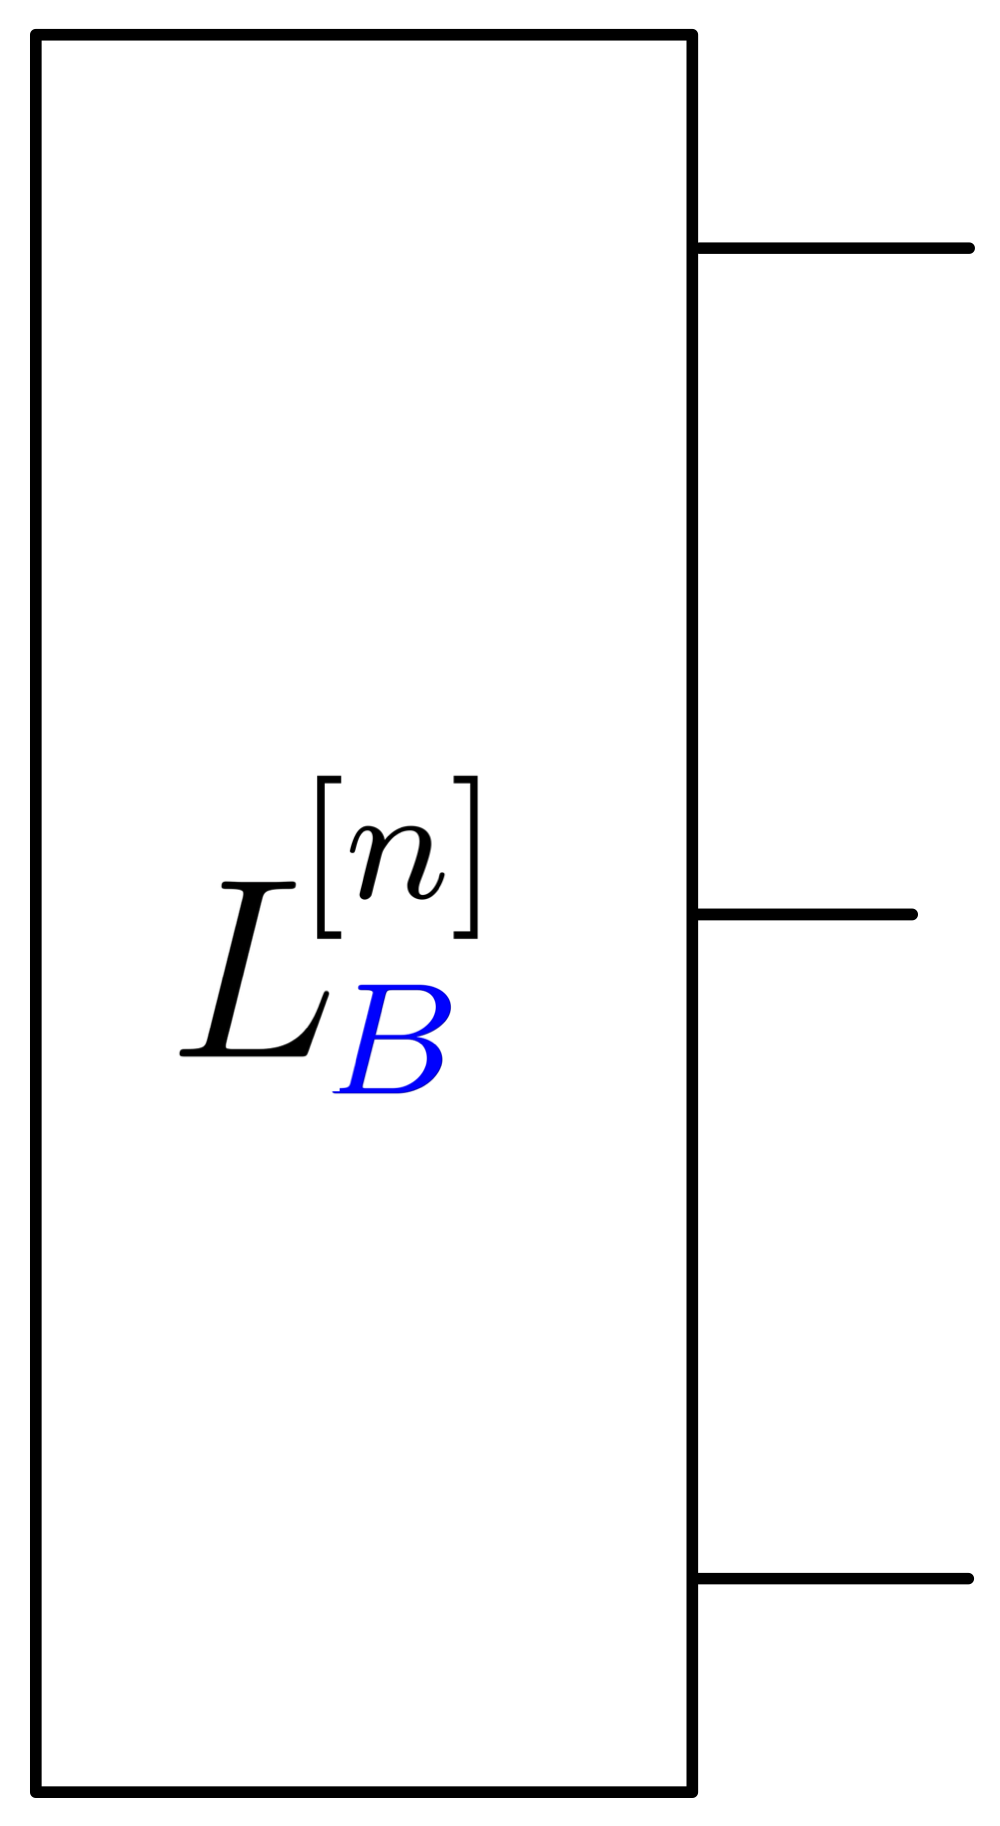
\includegraphics[height=3cm]{LB1.png}} 
	\:=\: 
	\raisebox{-0.5\height}{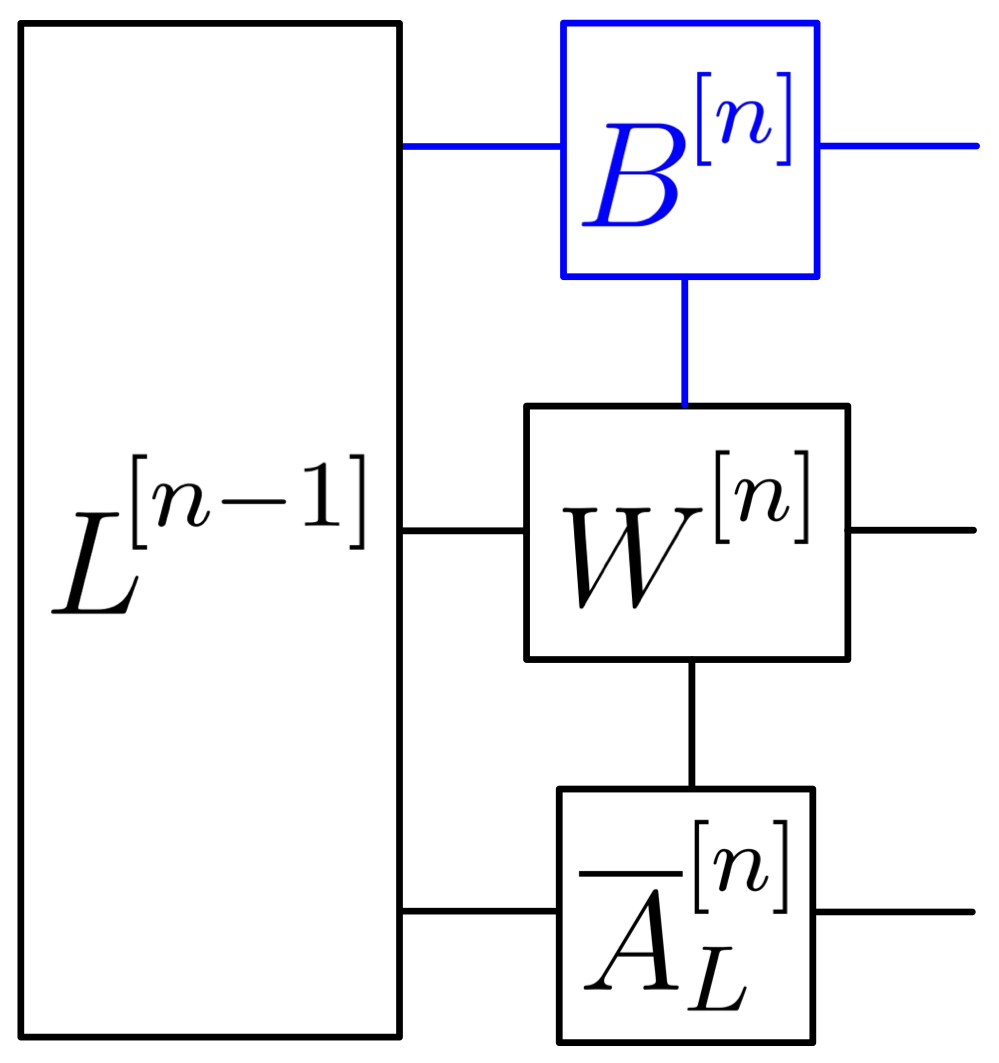
\includegraphics[height=3cm]{LB2.png}}
	\:+\:
	\raisebox{-0.5\height}{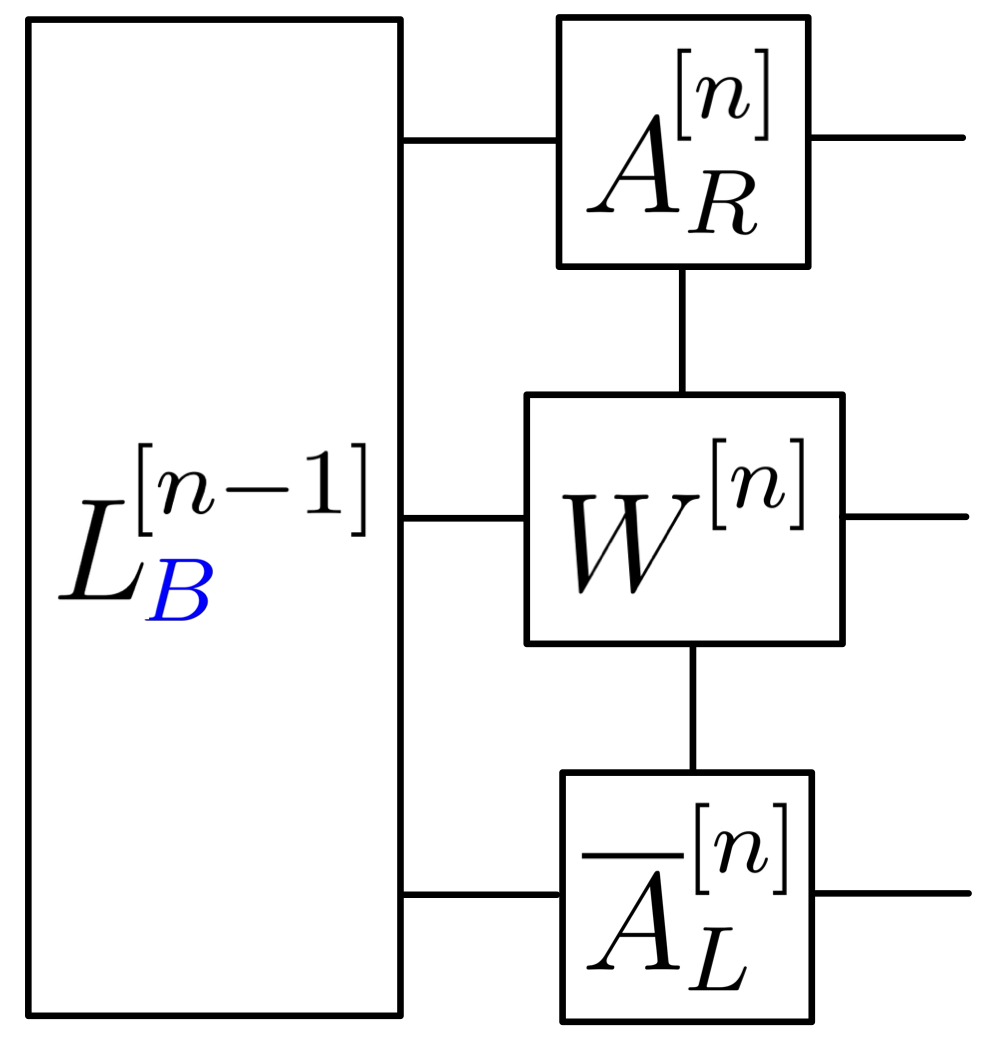
\includegraphics[height=3cm]{LB3.png}}
	\hspace{1em} \text{\scriptsize{$(n = 1, \ldots, N-1)$}},
\\[5em]
	\raisebox{-0.5\height}{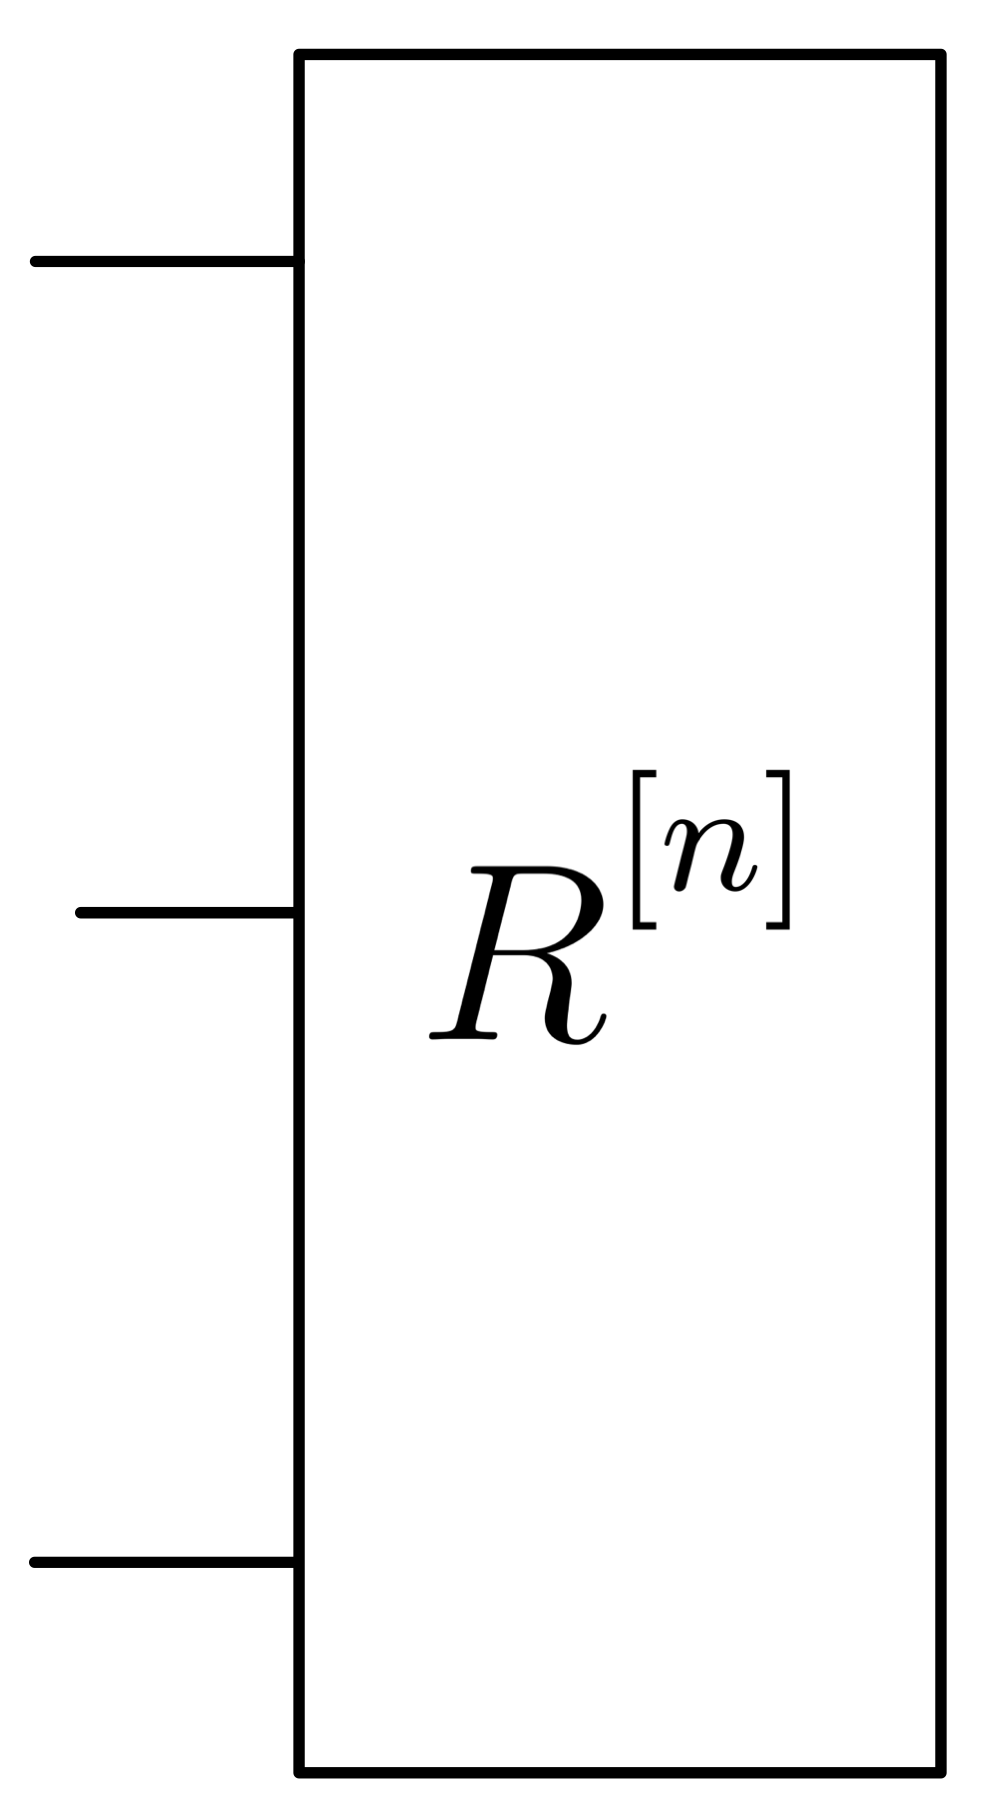
\includegraphics[height=3cm]{R1.png}} 
	\:=\:
	\raisebox{-0.5\height}{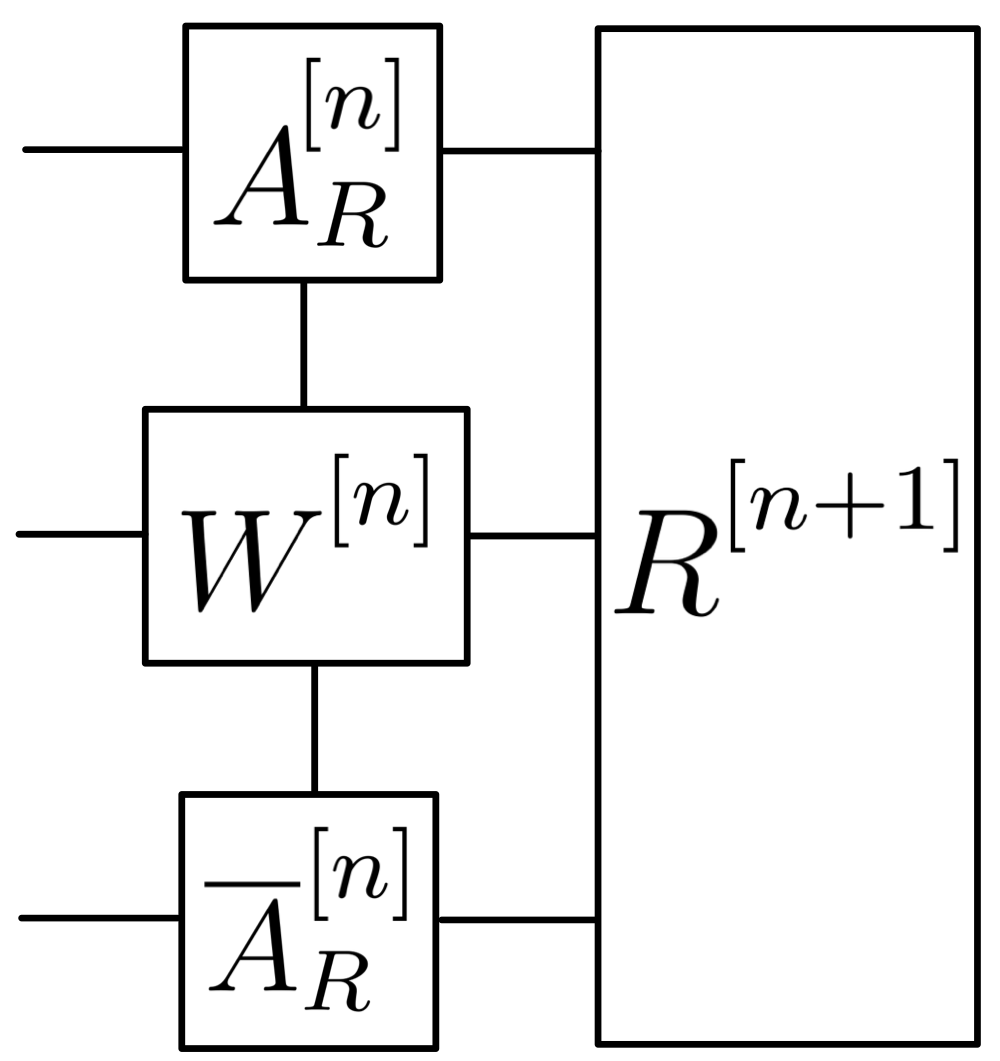
\includegraphics[height=3cm]{R2.png}} 
& ; &
	\raisebox{-0.5\height}{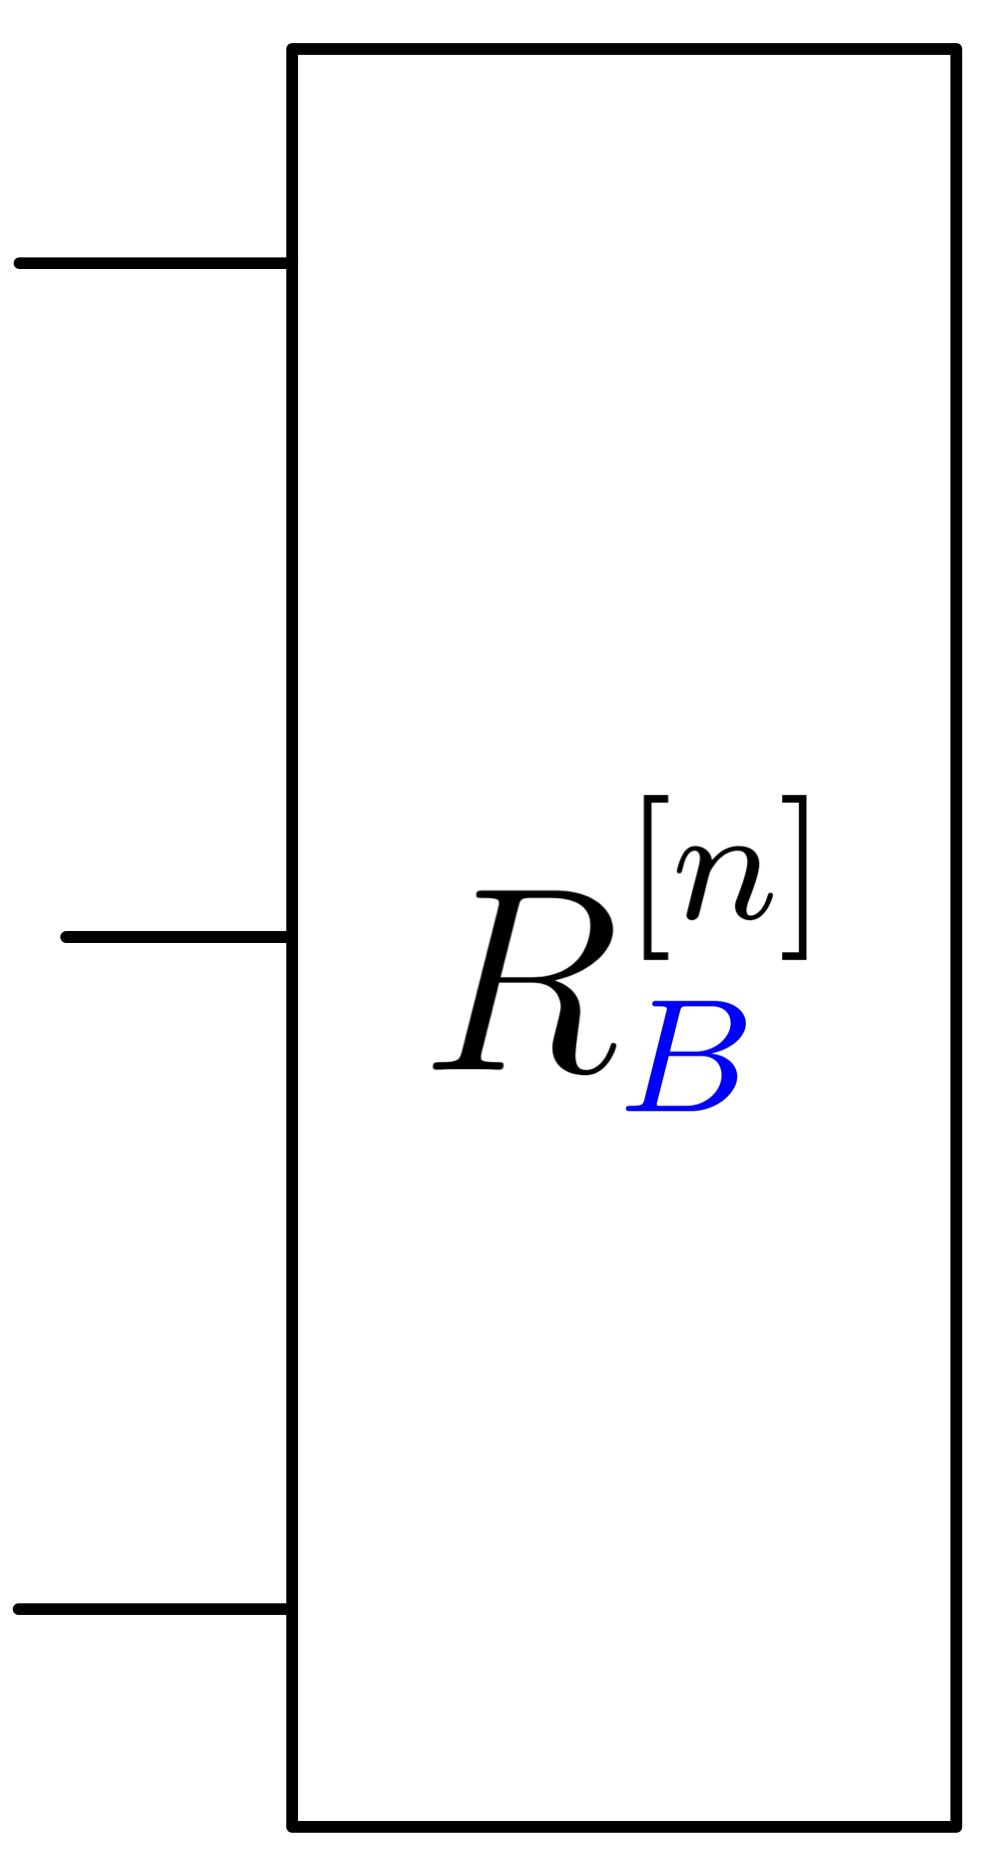
\includegraphics[height=3cm]{RB1.png}} 
	\:=\: 
	\raisebox{-0.5\height}{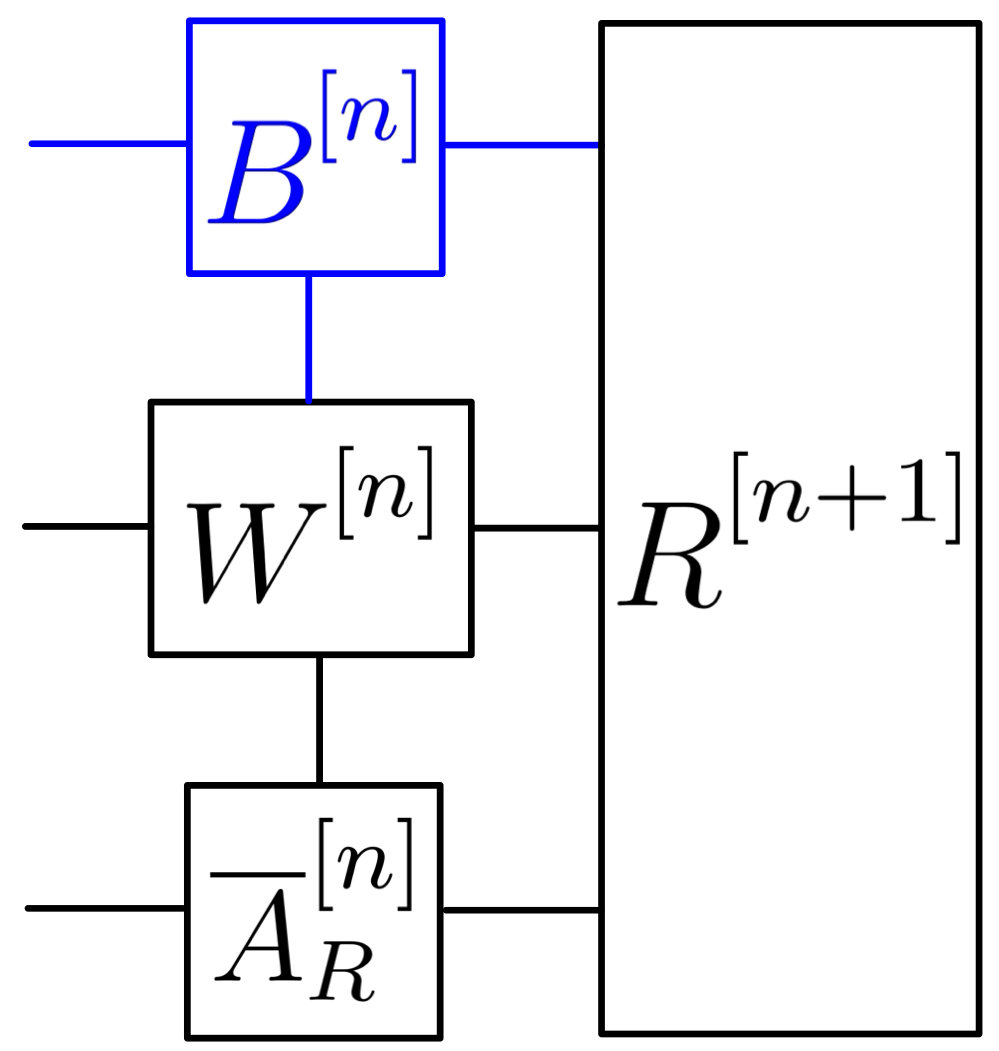
\includegraphics[height=3cm]{RB2.png}}
	\:+\:
	\raisebox{-0.5\height}{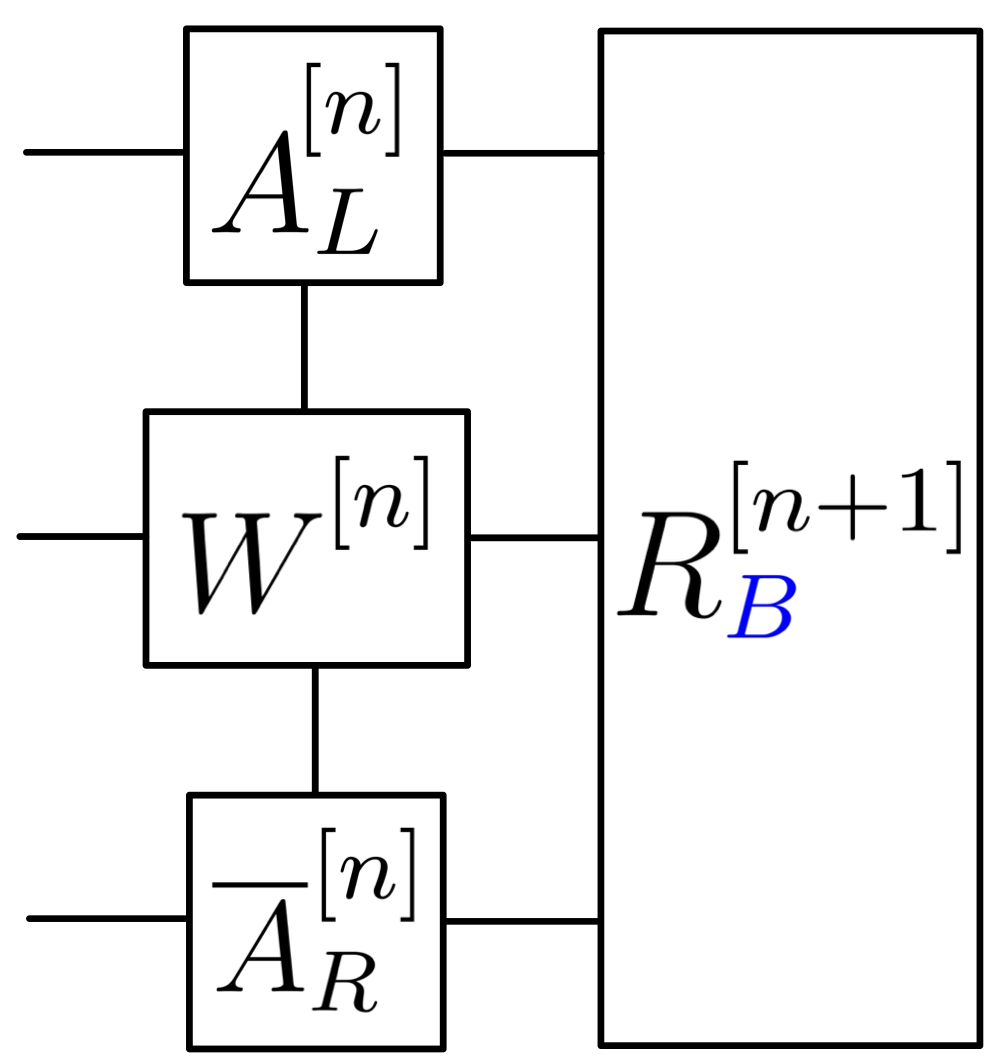
\includegraphics[height=3cm]{RB3.png}}
	\hspace{1em} \text{\scriptsize{$(n = N, \ldots, 2)$}}.
\end{array}
\end{equation}
After having solved \eqref{eq:effective_excitation_equation} with Lanczos for several algebraically smallest energy eigenvalues, we try to restore momentum as a good quantum number by diagonalizing the translation operator within each degenerate eigenspace. The successful result for $N = 20$ and $D_{\text{max}} = 64$ is shown in figure \ref{fig:excitations} (a). All excitations have a definite momentum $2\pi k /N$ for $k \in \{- \frac{N}{2}+1, ..., \frac{N}{2}\}$ and the corresponding energies agree with exact diagonalization. We also plot the single particle dispersion obtained from the exact mapping to free fermions in the odd parity sector. In the paramagnetic phase with representative transverse field value $g = 1.5$, the lowest lying excitations for all covered momenta lie perfectly on the dispersion curve. At the critical point $g = 1$ this is only roughly the case, as the distinction between different fermion parity sectors becomes more delicate for finite sizes. In the ferromagnetic phase, shown here for $g = 0.5$, the lowest lying excitations are topological domain walls, which are not accessible with a periodic Hamiltonian.
\end{samepage}

% effective translation operator
\newpage
\noindent \underline{Effective translation operator} \\[0.5em]
\noindent Knowing that momentum is a good quantum number, we can also directly target it by including the Hermitian sum of the translation operator in the effective eigenequation:
\begin{equation} \label{eq:effective_excitation_equation_T}
	\left[ H_{\text{eff}} - \alpha \left( e^{-i \frac{2\pi}{N}k} T_{\text{eff}} + e^{i \frac{2\pi}{N}k} T_{\text{eff}}^{\dagger} \right) \right] 
	 \tket{B} 
	 = \epsilon_k \tket{B}.
\end{equation}
The value for $\alpha > 0$ is chosen heuristically. It should be large enough to select the correct momentum sector, but not so large that it overrides the actual energy minimization. The tensor networks of the translation expectations values can be drawn as
\begin{align}
\begin{split}
	\textcolor{blue}{\tbra{\overline{B}}} &T_{\text{eff}} \textcolor{blue}{\tket{B}} \\
	&=
\end{split}
\end{align}
\vspace*{-0.5cm}
\begin{equation*}
	\raisebox{-0.45\height}{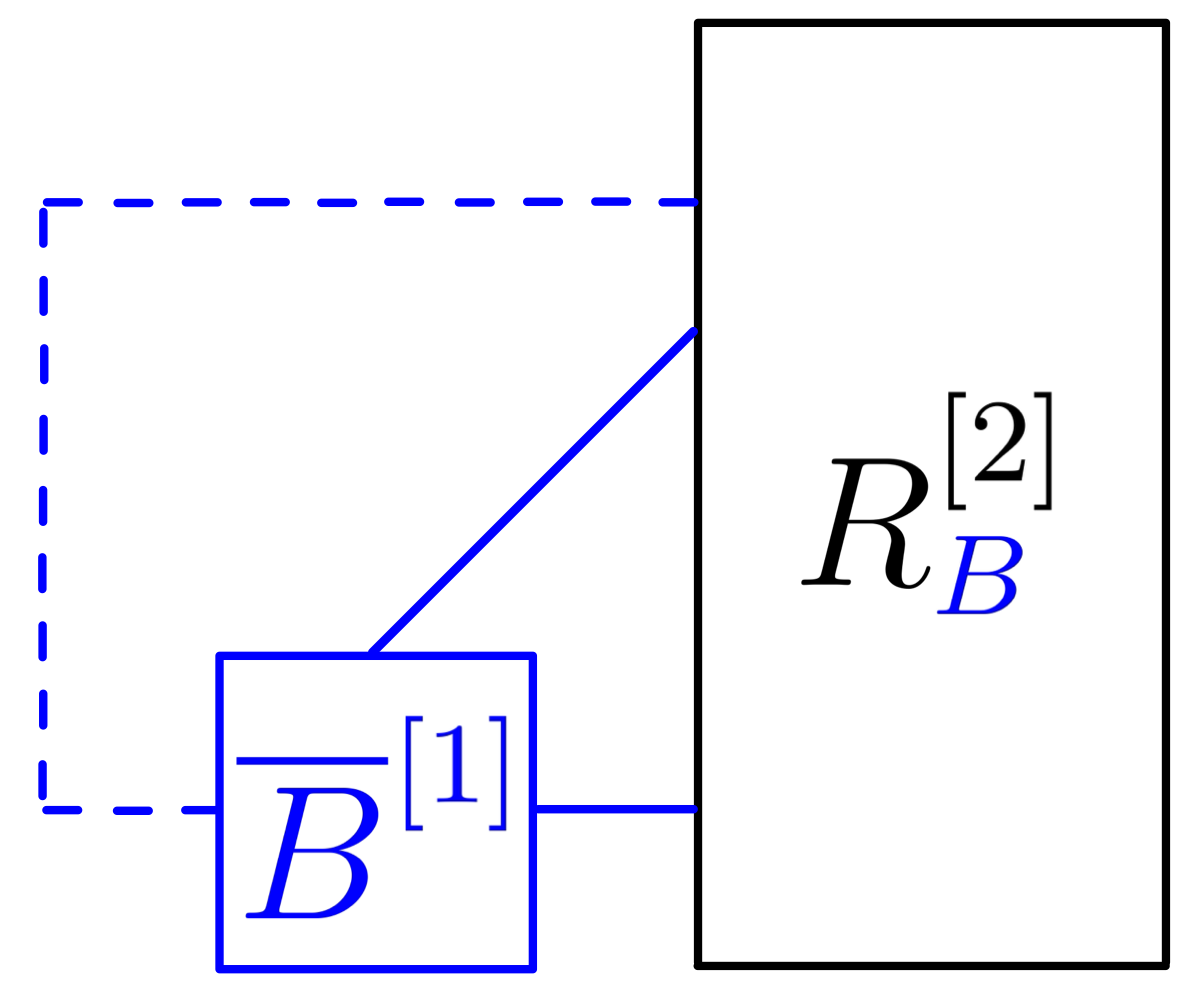
\includegraphics[height=2.cm]{T1.png}} 
	\:+\: \sum_{n=2}^N \left[
	\raisebox{-0.45\height}{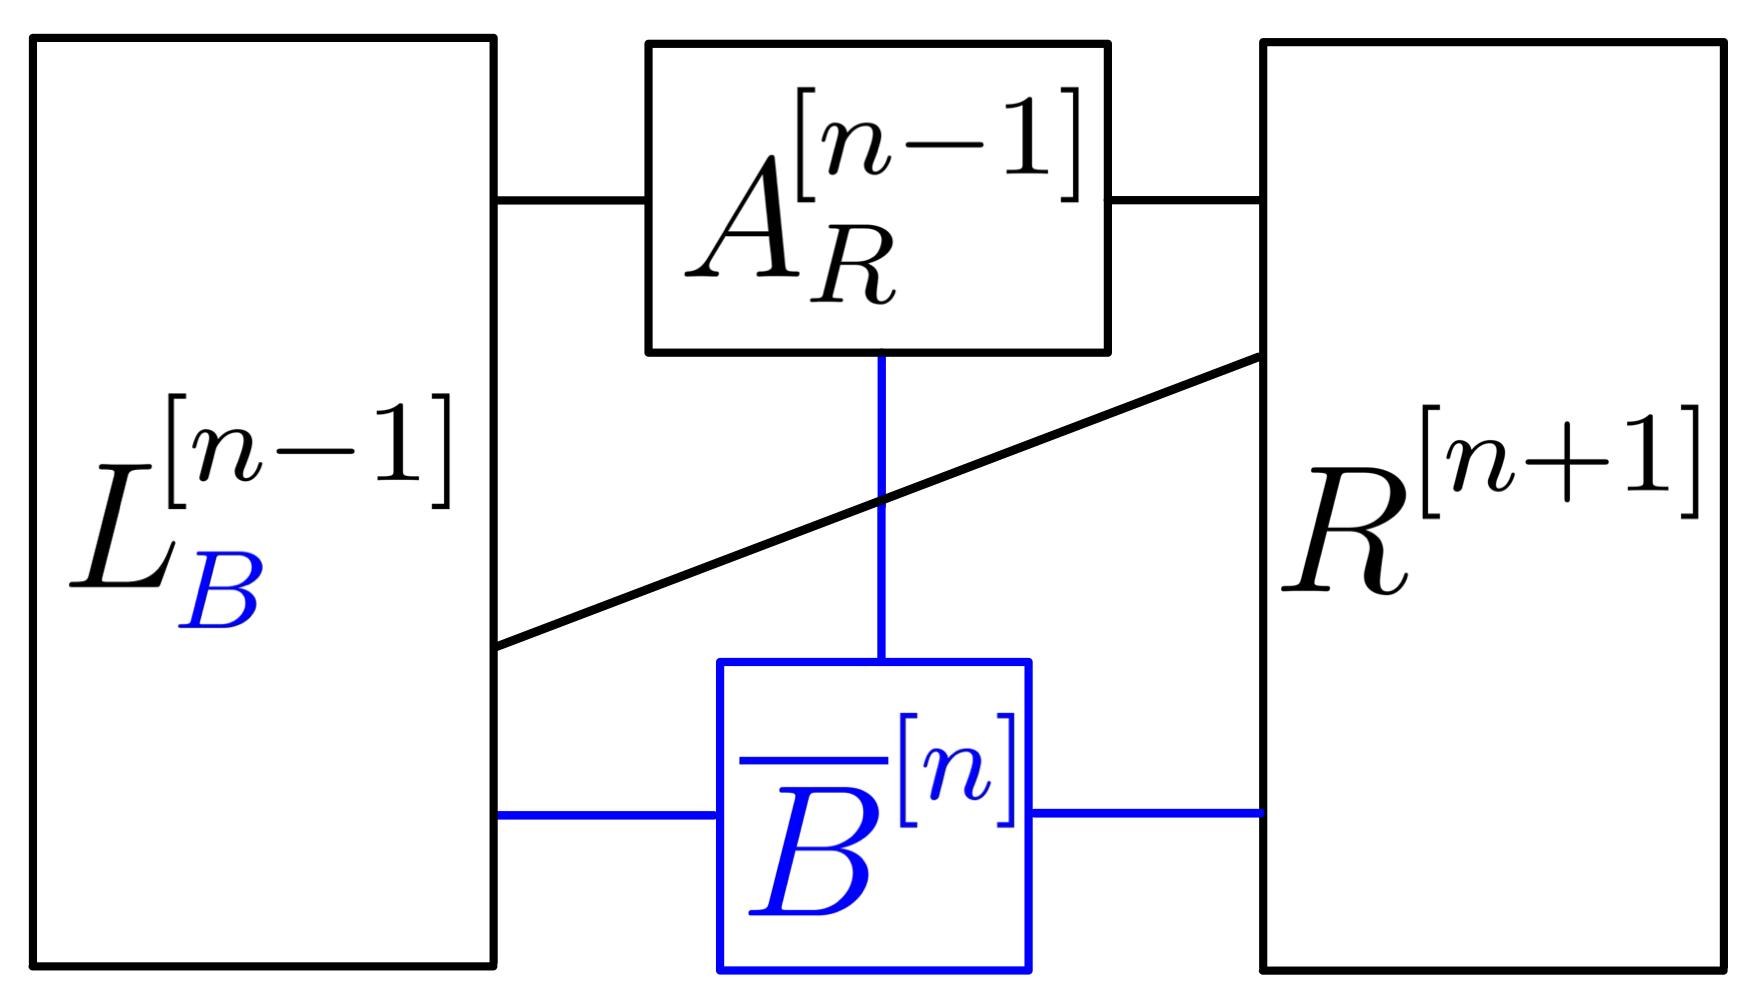
\includegraphics[height=2.cm]{T2.png}}
	+
	\raisebox{-0.45\height}{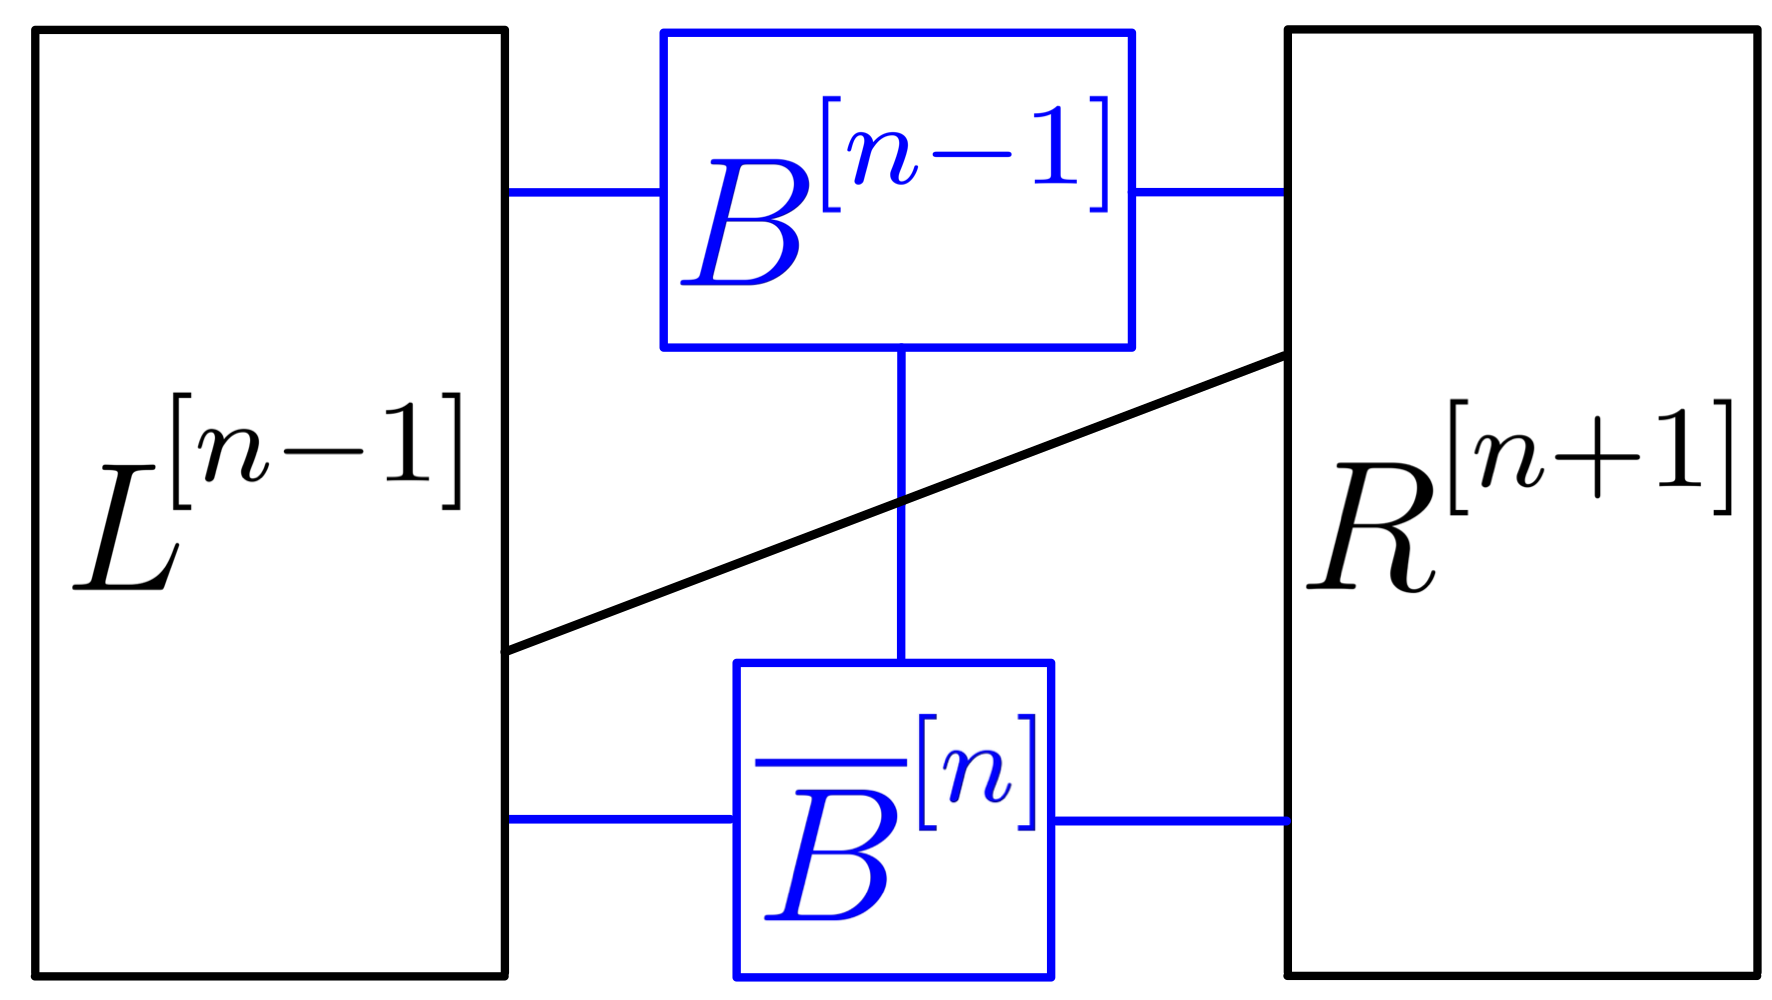
\includegraphics[height=2.cm]{T3.png}} 
	+ 
	\raisebox{-0.45\height}{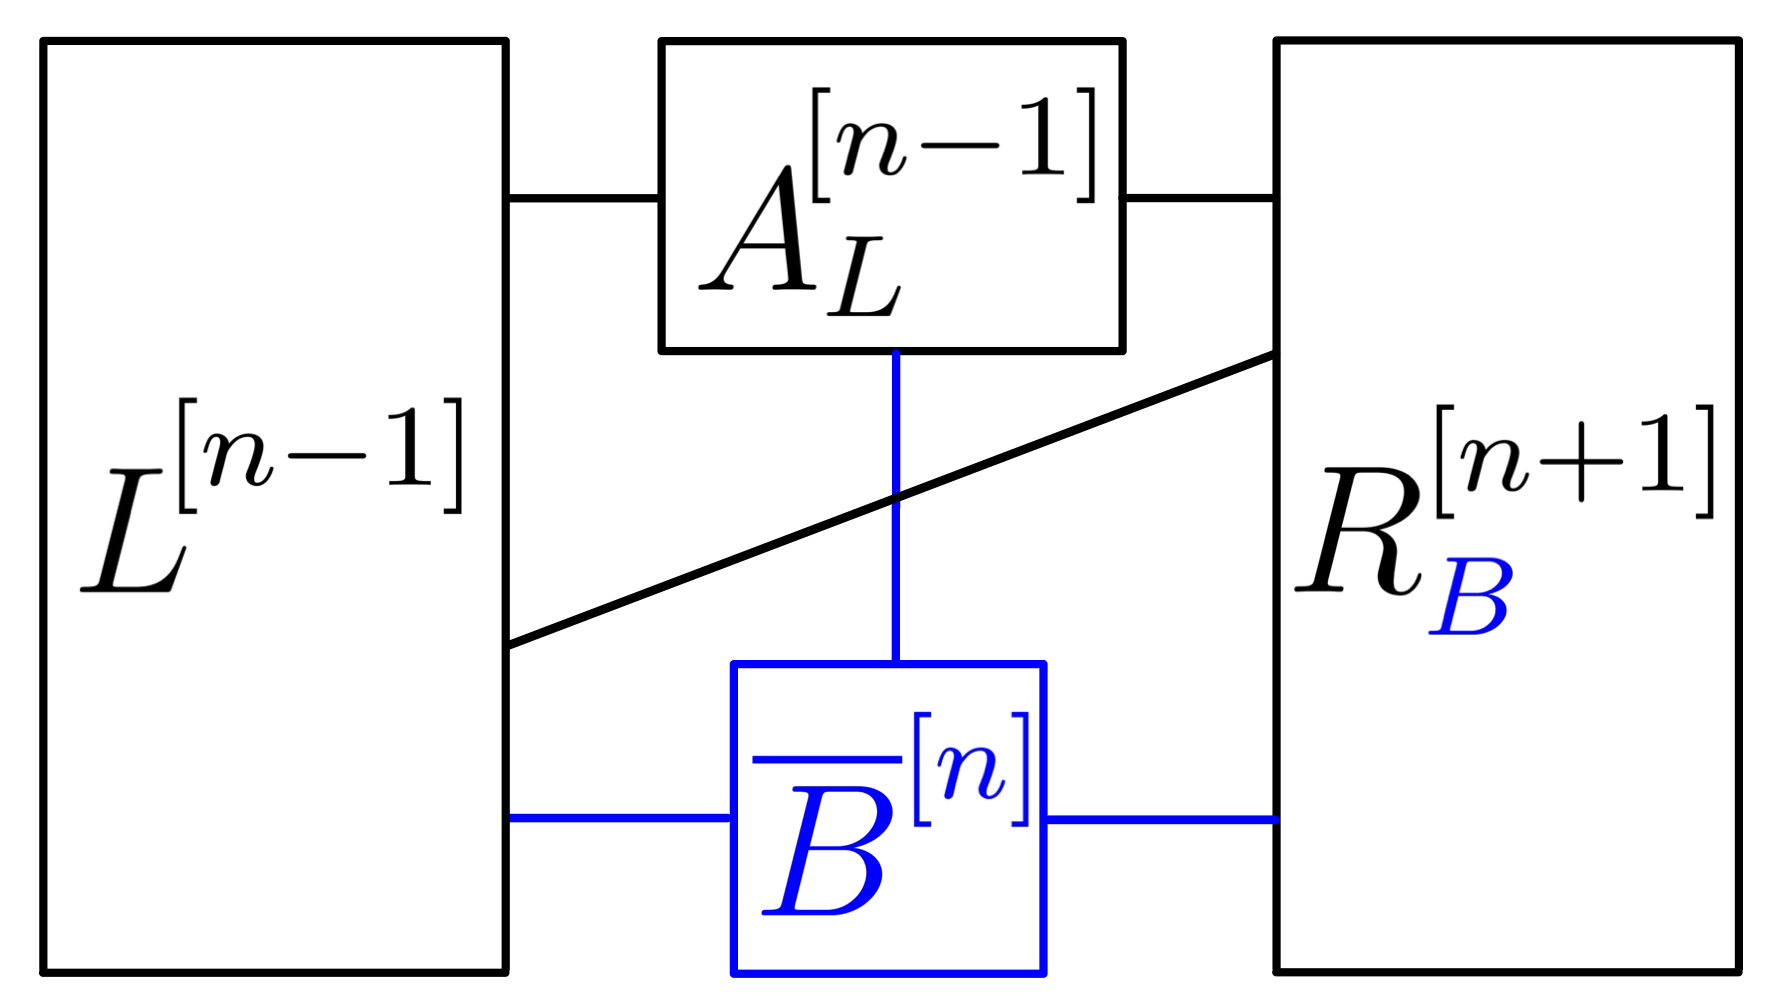
\includegraphics[height=2.cm]{T4.png}} 
	\right],
\end{equation*}
\vspace*{0.5cm}
\begin{align}
\begin{split}
	\textcolor{blue}{\tbra{\overline{B}}} &T_{\text{eff}}^{\dagger} \textcolor{blue}{\tket{B}} \\
	&=
\end{split}
\end{align}
\vspace*{-0.5cm}
\begin{equation*}
	\sum_{n=1}^{N-1} \left[
	\raisebox{-0.45\height}{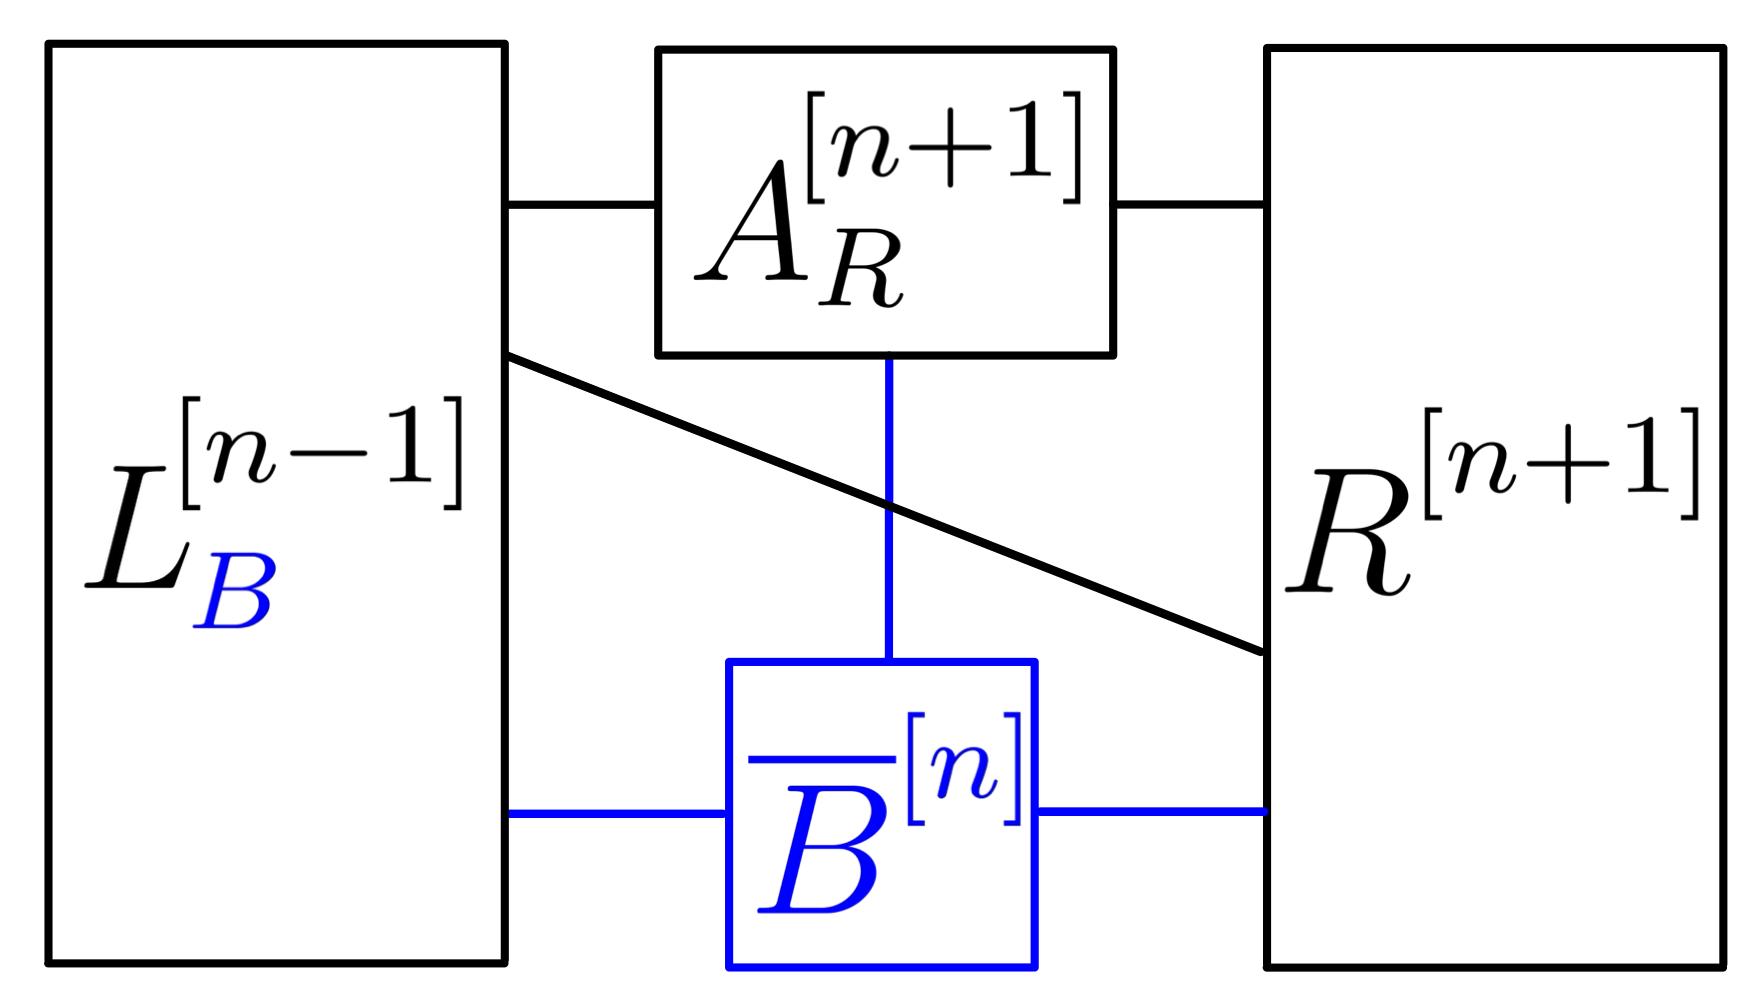
\includegraphics[height=2.cm]{Tdagger1.png}} 
	+
	\raisebox{-0.45\height}{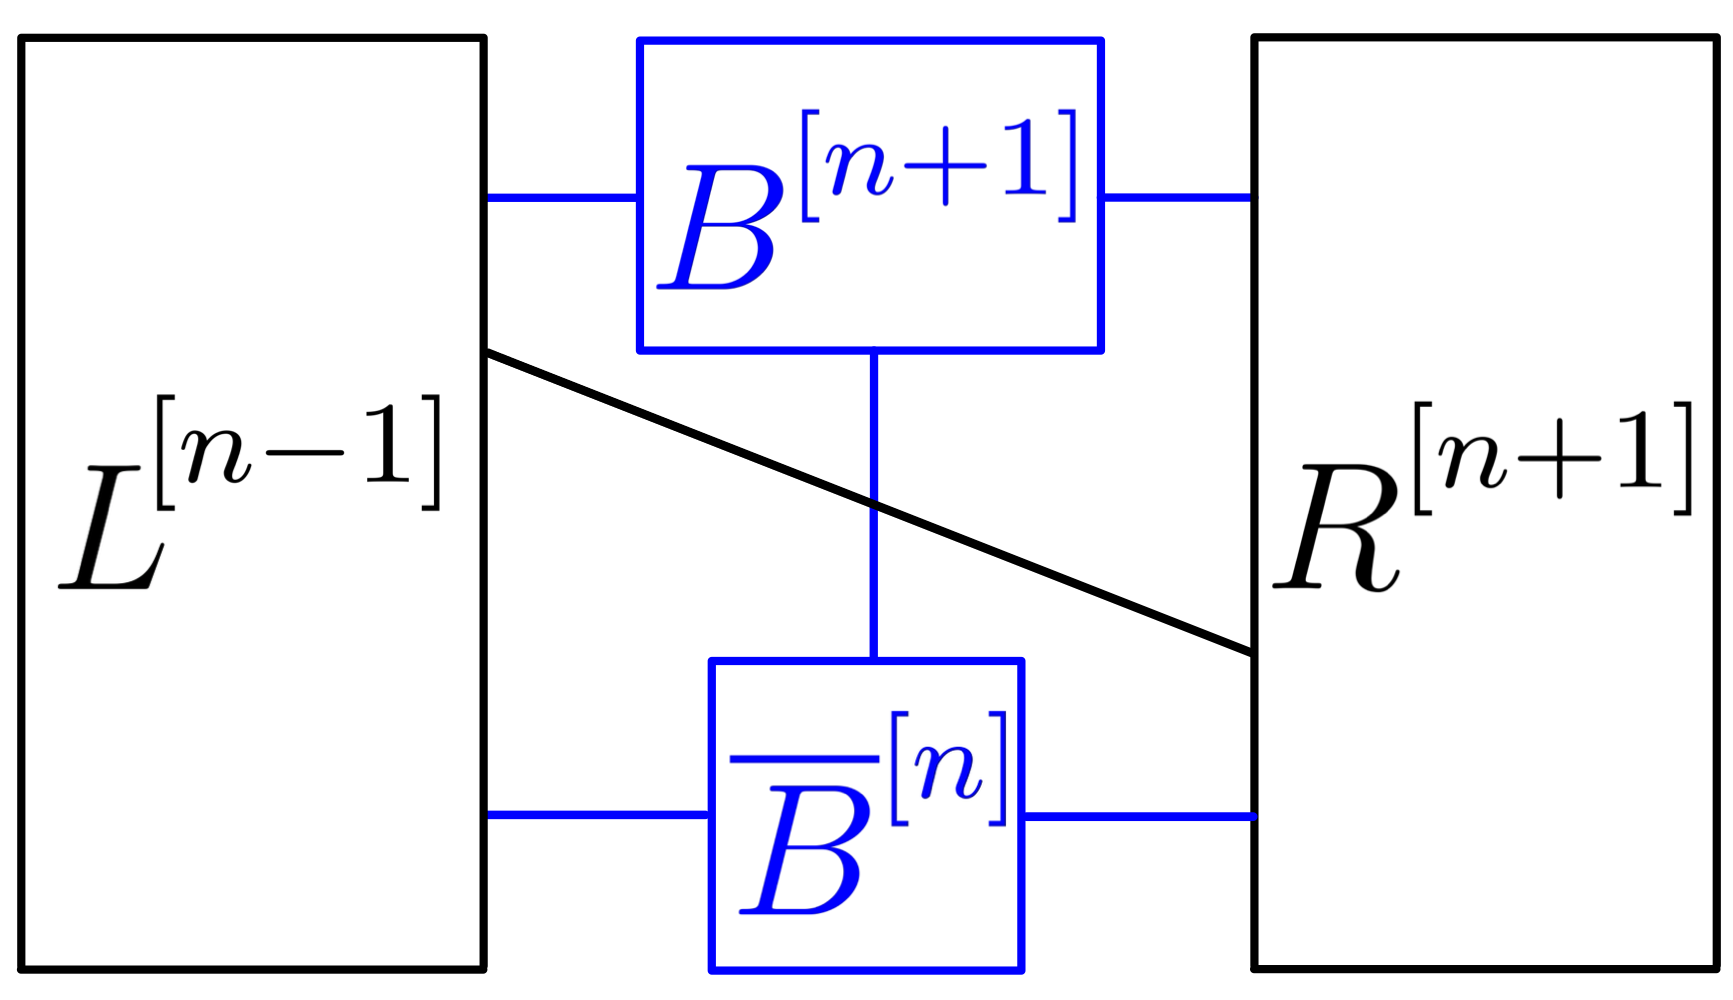
\includegraphics[height=2.cm]{Tdagger2.png}}
	+
	\raisebox{-0.45\height}{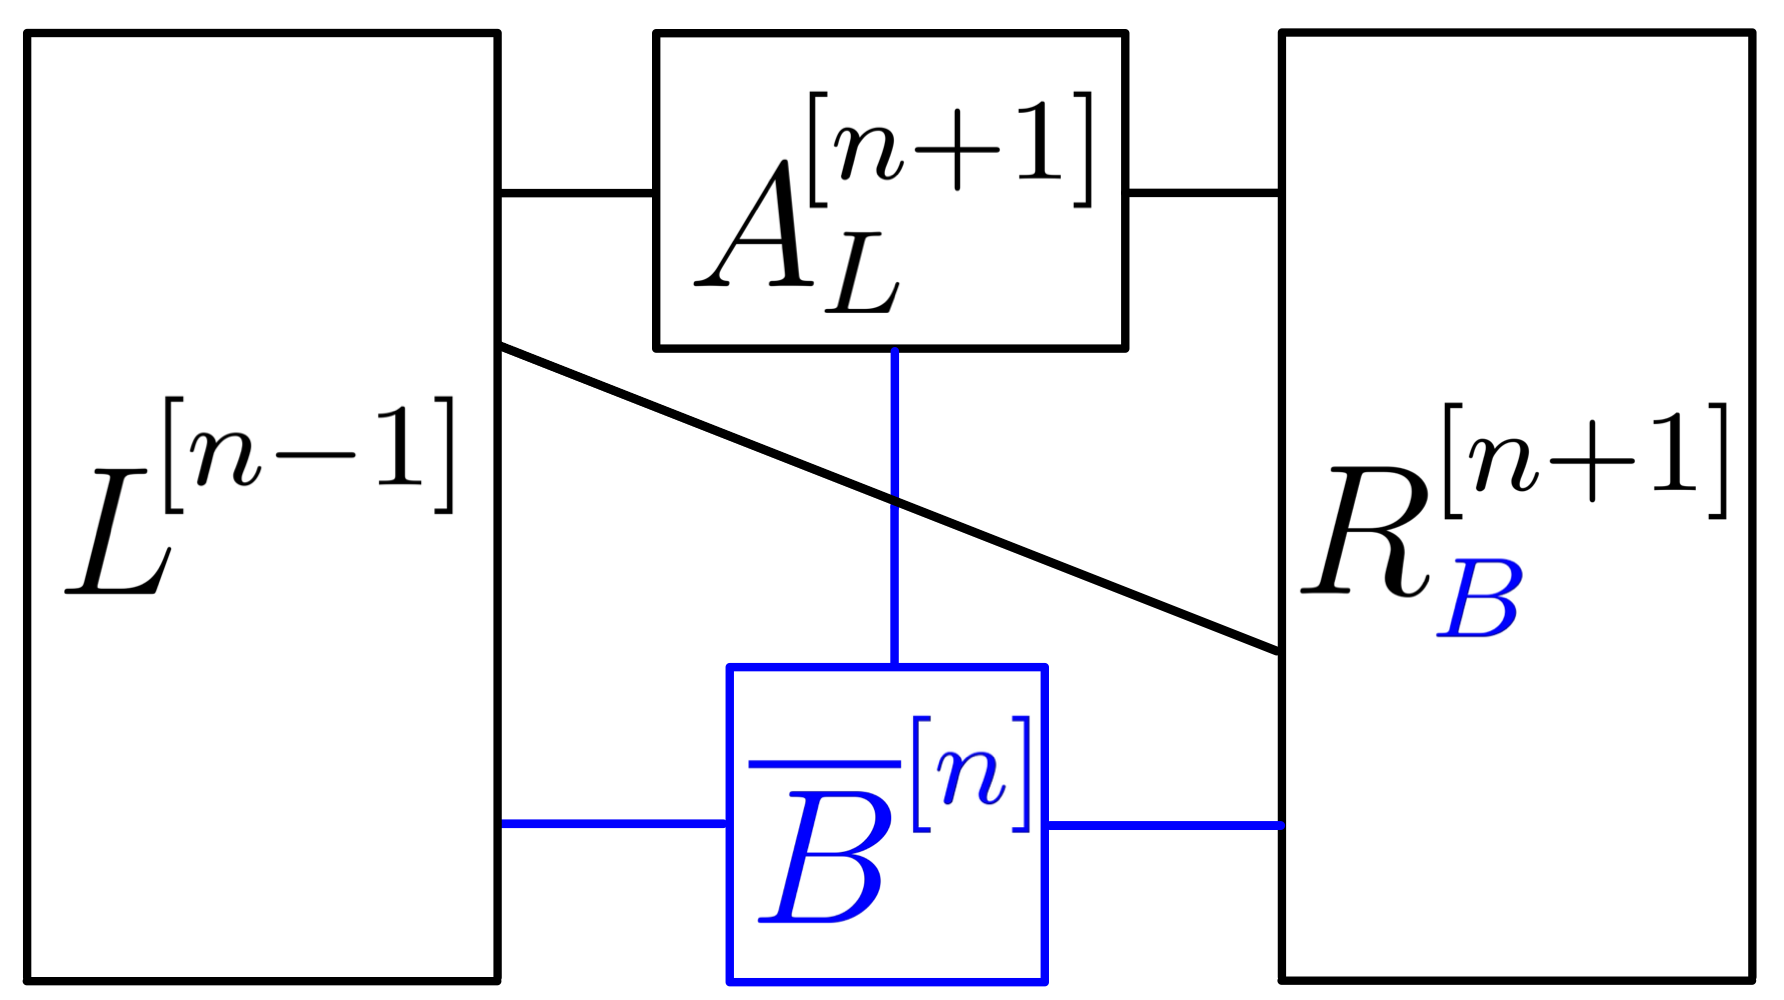
\includegraphics[height=2.cm]{Tdagger3.png}} 
	\right] 
	\:+\:
	\raisebox{-0.45\height}{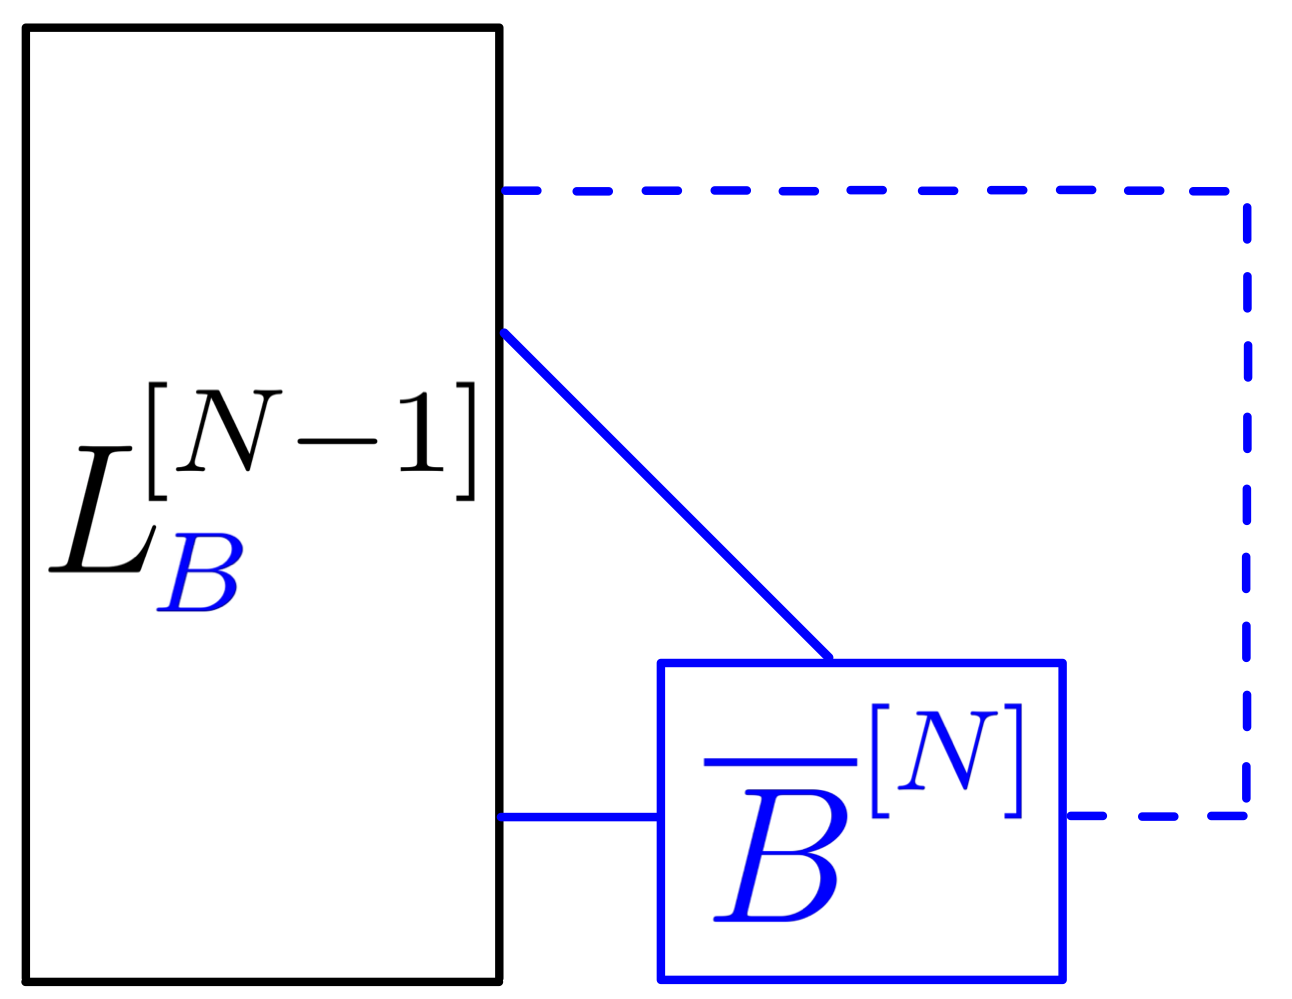
\includegraphics[height=2.cm]{Tdagger4.png}} \:.
\end{equation*}

\vspace*{1cm}

\noindent The boundary tensors are specified in appendix \ref{ch:extensive_tensor_network_diagrams}. The recursive principle of summing up the terms that
\begin{enumerate}
	\item[(i)] apply $B^{[n]}$ to the identity boundary,
	\item[(ii)] transfer the boundary for which all $B^{[m < n]}$ have already been applied,
\end{enumerate}
is the same as for $H_{\text{eff}}$. The results for the TFI model, again for the values $g = 0.5$, $g = 1.0$ and $g = 1.5$ are shown in figure \ref{fig:excitations} (b). The crucial difference to (a) lies in the direct access to the whole dispersion relation, in the sense that we don't have to compute multiple excitations of the same momentum to reach the first excitation of other momenta. \\[1em]

\newpage
\begin{figure}[H]
  \centering
  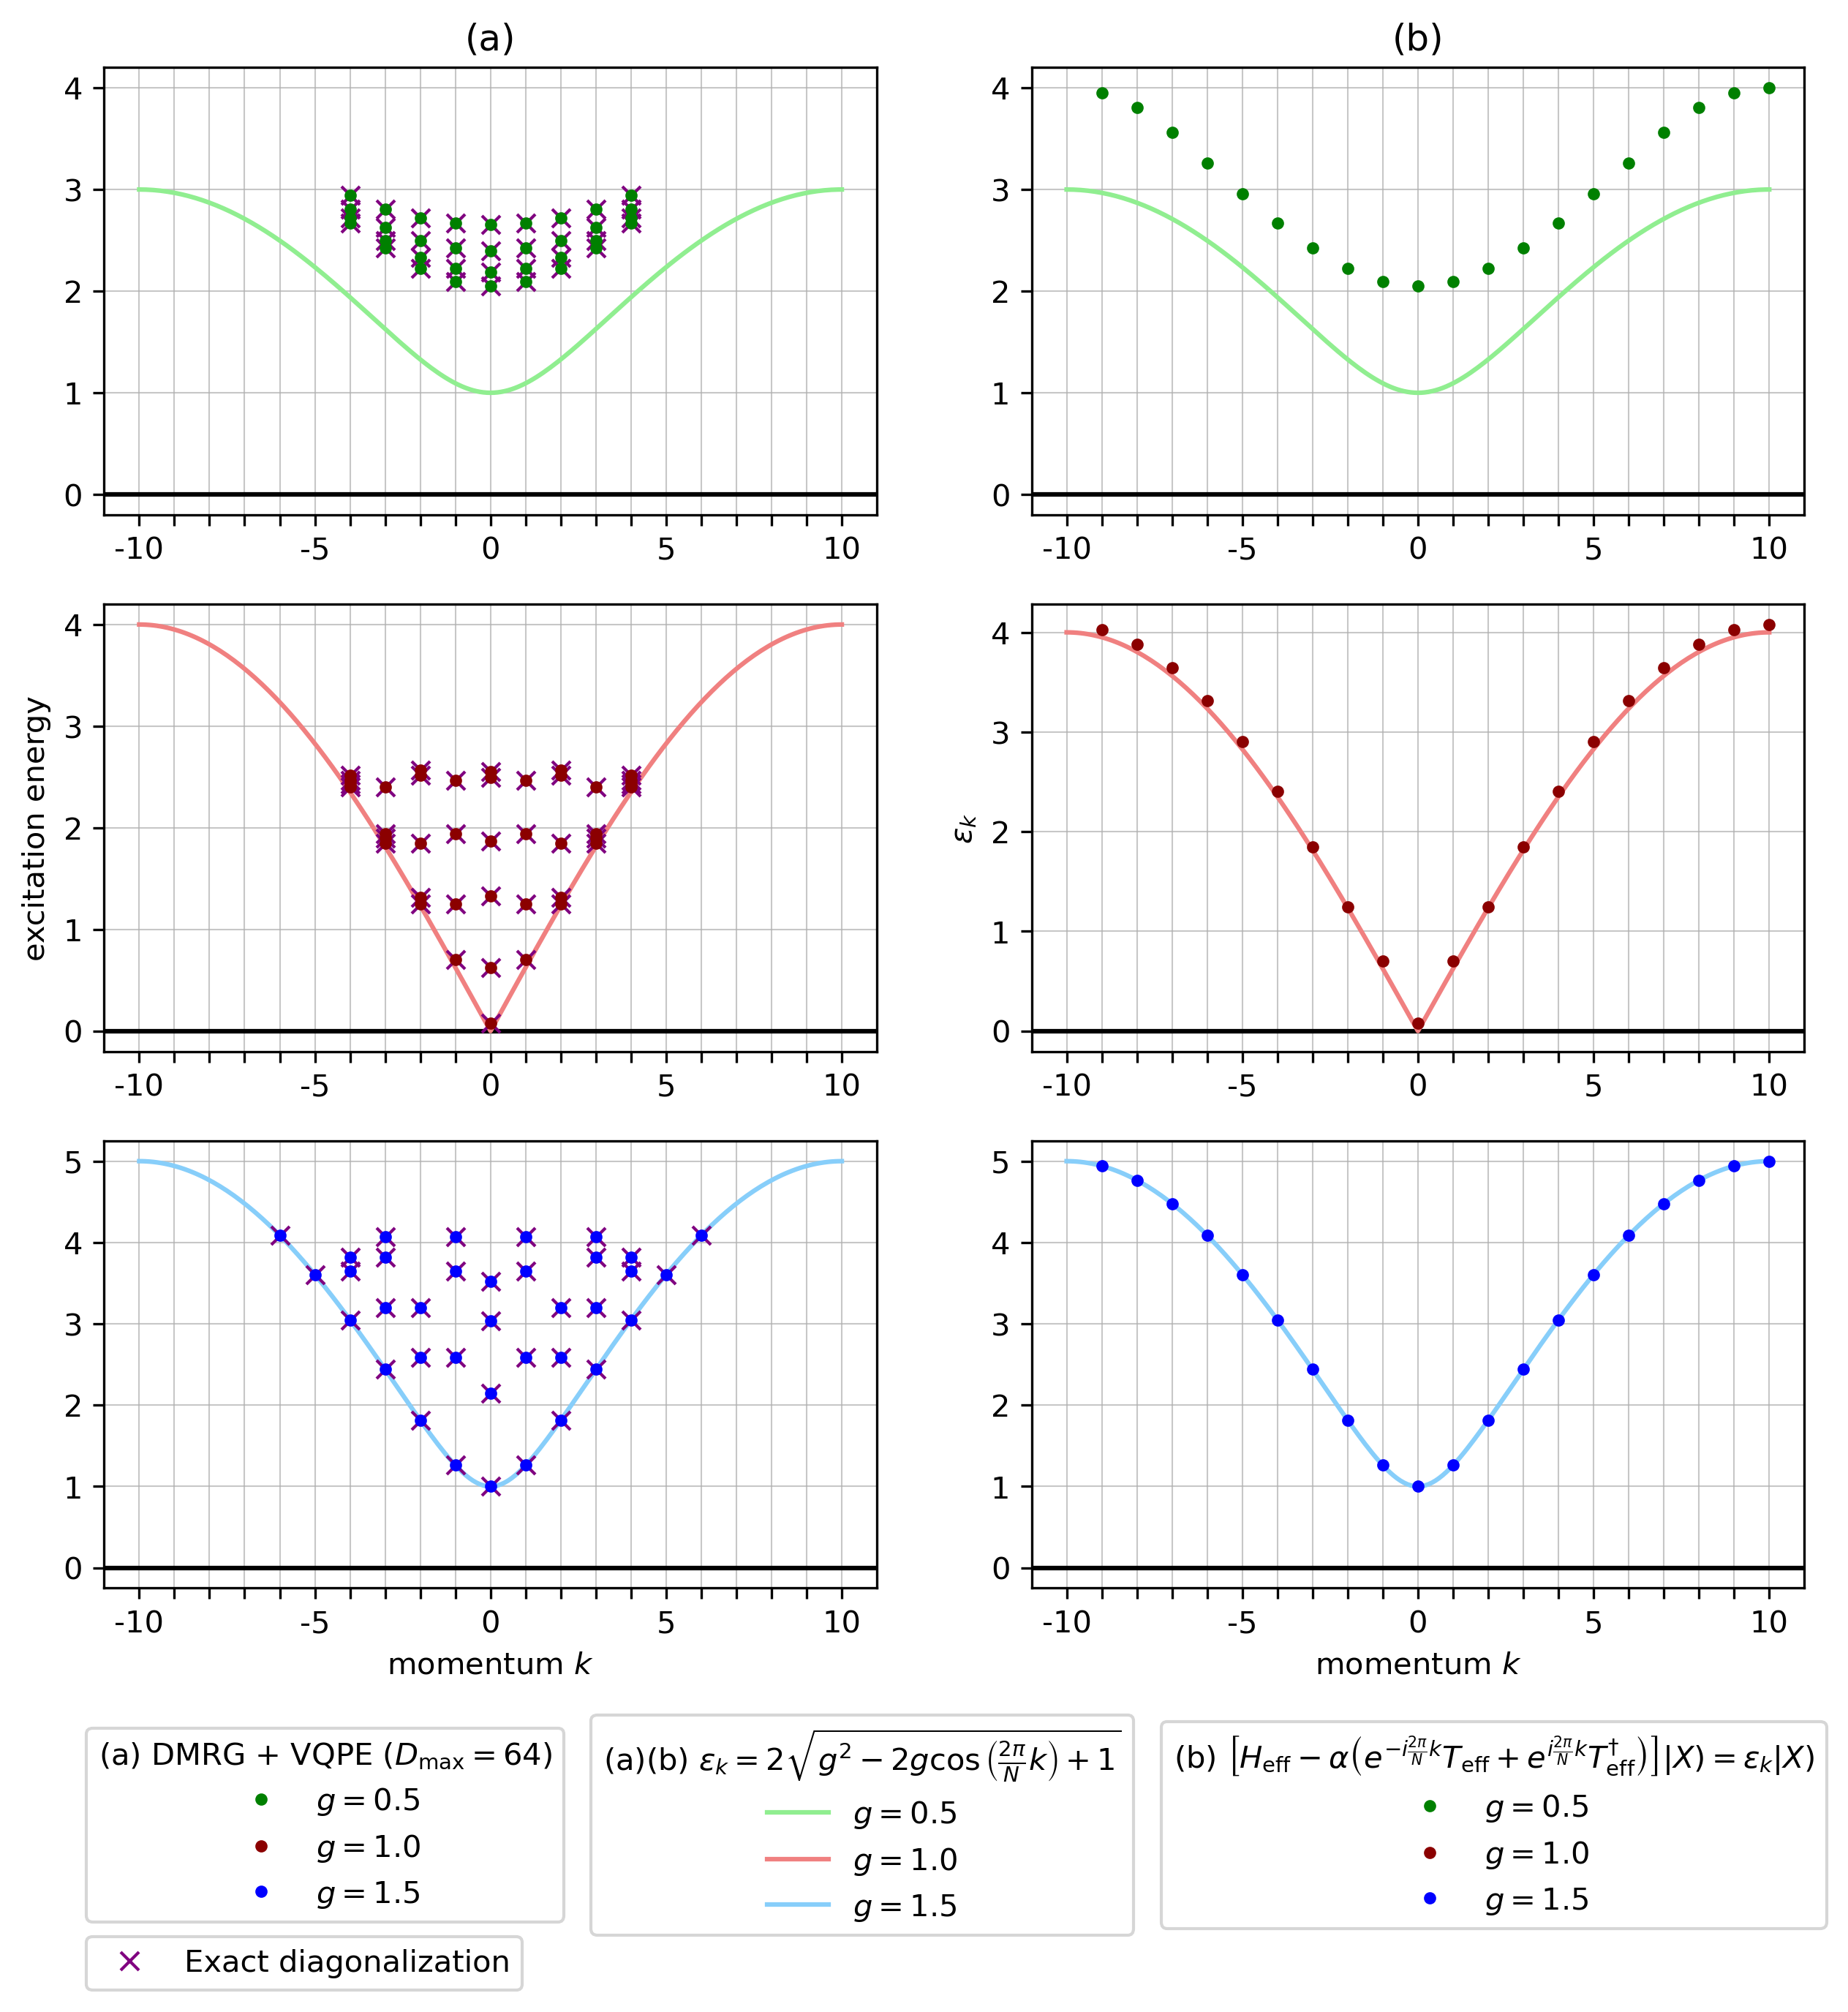
\includegraphics[width=1.0\linewidth]{excitations.png}
  \caption{TFI benchmark for variational quasiparticle excitations on top of a finite MPS ground state. We choose PBC for the Hamiltonian, chain length $N = 20$ and maximal bond dimension $D_{\text{max}} = 64$. On the left side (a), we first diagonalize the Hamiltonian and afterwards the translation operator within each energy-degenerate eigenspace. We compare the results to exact diagonalization and the single particle dispersion obtained from the Jordan-Wigner mapping to free fermions (in the odd parity sector). The lowest lying domain wall excitations in the ferromagnetic phase $g < 1$ are not eigenstates of the periodic Hamiltonian. The right side (b) shows the benchmark for quasiparticle excitations variational in energy and momentum. We include the Hermitian translation operator $- \alpha ( e^{-i 2\pi k / N} T_{\text{eff}} + e^{i 2\pi k / N} T_{\text{eff}}^{\dagger} )$ directly in the effective eigenvalue equation. This frees us from computing multiple excitations of the same momentum, whose energies lie below the first excitation of other momenta.}
\label{fig:excitations}
\end{figure}


% local energies
\noindent \underline{Local energies} \\[0.5em]
Going from periodic to open boundary conditions for the Hamiltonian, it does no longer commute with the translation operator. As a consequence, the excitations cannot be momentum eigenstates anymore. Nevertheless, we expect standing wave configurations of the very same dressed particle. 
This can be understood easiest in the single particle picture, known from the perturbative approach in section \ref{sec:tfi_perturbation_theory}. For the effective Hamiltonian 
\begin{equation}
	H_{\text{eff}} =  \mu \sum_n \ket{n} \bra{n} - t \sum_n \left( \ket{n} \bra{n+1} + \ket{n+1} \bra{n} \right),
\end{equation}
we want to compare the local energies, i.e. the expectation values of
\begin{equation}
	h_{n, n+1} =  \frac{\mu}{2} \ket{n} \bra{n} + \frac{\mu}{2} \ket{n+1} \bra{n+1} - t \left( \ket{n} \bra{n+1} + \ket{n+1} \bra{n} \right)
\end{equation}
for the respective eigenstates. For both boundary conditions, they can be labeled by a wave number $p$ such that
\begin{equation}
	H_{\text{eff}} = \sum_p \epsilon_p \ket{p} \bra{p} \text{ with } \epsilon_p =  \mu - 2t \cos(p).
\end{equation}
For the TFI model with large $g$ and $J = 1$, on-site energy and hopping take the values $\mu = 2g$ and $t = 1$. \\[0.5em]
\noindent 1) PBC: The eigenstates are plane waves
\begin{equation}
	\ket{p} = \frac{1}{\sqrt{N}} \sum_n e^{ipn} \ket{n} \: \text{ with }\: p = \frac{2 \pi}{N} k \:\text{ and }\: k = 0, \pm 1, \ldots, \pm \left( \frac{N}{2}-1 \right), \frac{N}{2}.
\end{equation}
While the pure momentum states $\ket{\pm p}$ have constant local energy $\langle h_{n, n+1} \rangle = \epsilon_p / N = \epsilon_{-p} / N$, their equal weighted superpositions show spatial oscillations:
\begin{align*}
	& \ket{p+} = \frac{1}{\sqrt{2}} \left( \ket{p} + \ket{-p} \right) = \sqrt{\frac{2}{N}} \sum_n \cos(pn) \ket{n}, \\
	& \langle h_{n, n+1} \rangle_+ 
	= \left[ 
	\mu \cos^2 \left( \frac{2 \pi k n}{N} \right) 
	+ \mu \cos^2 \left( \frac{2 \pi k (n+1)}{N}  \right) 
	- 4t \cos \left( \frac{2 \pi k n}{N} \right) \cos \left( \frac{2 \pi k(n+1)}{N} \right) 
	\right] / N, \\
	& \ket{p-} = \frac{1}{\sqrt{2}} \left( \ket{p} - \ket{-p} \right) = i\sqrt{\frac{2}{N}} \sum_n \sin(pn) \ket{n}, \\
	& \langle h_{n, n+1} \rangle_- 
	= \left[ 
	\mu \sin^2 \left( \frac{2 \pi k n}{N} \right) 
	+ \mu \sin^2 \left( \frac{2 \pi k (n+1)}{N} \right) 
	- 4t \sin \left( \frac{2 \pi k n}{N} \right) \sin \left( \frac{2 \pi k (n+1)}{N}  \right)
	\right] / N.
\end{align*}

\vspace*{1em}
\noindent 2) OBC: For Dirichlet "vanishing edge" conditions $\psi_0 = \psi_{N+1} = 0$, the solutions are standing waves with nodes at the boundaries. They provide a finer resolution in wave numbers $k$, which are confined to half the Brillouin zone:
\begin{align*}
	& \ket{p} = \sqrt{\frac{2}{N+1}} \sum_n \sin(pn) \ket{n} \:\text{ with }\: p = \frac{\pi}{N+1} k \:\text{ and }\: k = 1, \ldots N, \\
	& \langle h_{n, n+1} \rangle 
	= \left[ 
	 \mu \sin^2 \left( \frac{\pi k n}{N+1} \right) 
	+ \mu \sin^2 \left(  \frac{\pi k (n+1)}{N+1} \right) 
	- 4t \sin \left( \frac{\pi k n}{N+1} \right) \sin \left( \frac{\pi k (n+1)}{N+1} \right)
	\right] / (N+1).
\end{align*}

\begin{figure}[H]
  \centering
  \includegraphics[width=1.0\linewidth]{excitations_local_energies.png}
  \caption{TFI benchmark for the quasiparticle excitation waves with PBC and OBC. For $g = 1.5$, $N = 100$ and $D_{\text{max}} = 64$ we compute the four lowest lying MPS quasiparticle excitations. For OBC the local energies describe standing wave configurations with nodes at the boundary and corresponding wave numbers confined to half the Brillouin zone. For PBC the momenta are distributed symmetrically in both halves of the Brillouin zone and the superpositions of $\pm k$ eigenstates show periodic oscillations in the local energies, without nodes.}
 \label{fig:excitations_local_energies}
\end{figure}

\vspace*{1.5em}
\noindent For an MPS quasiparticle excitation \eqref{eq:excitation_ansatz}, the local energy expectation value leads to the double sum 
\begin{equation}
	\bra{\psi(\overline{B}; \overline{A})} h^{[n, n+1]} \ket{\psi(B; A)}
	=
	\sum_{m, \Tilde{m}}\bra{\psi(\overline{B}^{[\Tilde{m}]}; \overline{A})} h^{[n, n+1]} \ket{\psi(B^{[m]}; A)}.
\end{equation}
We efficiently combine the terms where $B^{[m]}$ and/or $\overline{B}^{[\Tilde{m}]}$ are at positions $m, \Tilde{m} \notin \{n, n+1\}$ in the following environment tensors, all computed recursively starting from zero tensors at $n = 0$ or $n = N+1$:
\begin{equation} \label{eq:local_energies_boundary_tensors}
	 \raisebox{-0.5\height}{\includegraphics[height=3cm]{hLBB1.png}}
	 \:=\:
	 \raisebox{-0.5\height}{\includegraphics[height=3cm]{hLBB2.png}}
	 \:+\:
	 \raisebox{-0.5\height}{\includegraphics[height=3cm]{hLBB3.png}}
	 \hspace{1em} \text{\scriptsize{$(n = 1, \ldots, N-2)$}},
\end{equation}
\begin{equation*}
	 \raisebox{-0.5\height}{\includegraphics[height=3cm]{hRB1.png}}
	 \:=\:
	 \raisebox{-0.5\height}{\includegraphics[height=3cm]{hRB2.png}}
	 \:+\:
	 \raisebox{-0.5\height}{\includegraphics[height=3cm]{hRB3.png}}
\:\: ; \:\:\:\:
	 \raisebox{-0.5\height}{\includegraphics[height=3cm]{hRB4.png}}
	 \:=\:
	 \raisebox{-0.5\height}{\includegraphics[height=3cm]{hRB5.png}}
	 \:+\:
	 \raisebox{-0.5\height}{\includegraphics[height=3cm]{hRB6.png}}
\:\: ;
\end{equation*}
\begin{equation*}
	 \raisebox{-0.5\height}{\includegraphics[height=3cm]{hRBB1.png}}
	 \:=\:
	 \raisebox{-0.5\height}{\includegraphics[height=3cm]{hRBB2.png}}
	 \:+\:
	 \raisebox{-0.5\height}{\includegraphics[height=3cm]{hRBB3.png}}
	 \:+\:
	 \raisebox{-0.5\height}{\includegraphics[height=3cm]{hRBB4.png}}
	 \:+\:
	 \raisebox{-0.5\height}{\includegraphics[height=3cm]{hRBB5.png}}
	 \hspace{1em} \text{\scriptsize{$(n = N, \ldots, 3)$}}.
\end{equation*}

\vspace*{1em}
\noindent With these boundary tensors the higher level tensor diagram reads
\begin{equation} \label{eq:local_energies}
\begin{array}{cccccc}
	& & & \bra{\psi(\textcolor{blue}{\overline{B}}; \overline{A})} h^{[n, n+1]} \ket{\psi(\textcolor{blue}{B}; A)} & & 
\\[0.5em]
	& & & = & &
\\[0.5em]
	& & & \raisebox{-0.5\height}{\includegraphics[height=3cm]{h1.png}} & & 
\\[5em]
	\:+\: 
	& \raisebox{-0.5\height}{\includegraphics[height=3cm]{h2.png}} 
	& \:+\: 
	& \raisebox{-0.5\height}{\includegraphics[height=3cm]{h3.png}}
	& \:+\: 
	& \raisebox{-0.5\height}{\includegraphics[height=3cm]{h4.png}} 
\\[5em]
	\:+\: 
	& \raisebox{-0.5\height}{\includegraphics[height=3cm]{h5.png}} 
	& \:+\: 
	& \raisebox{-0.5\height}{\includegraphics[height=3cm]{h6.png}}
	& \:+\: 
	& \raisebox{-0.5\height}{\includegraphics[height=3cm]{h7.png}} 
\\[5em]
	\:+\: 
	& \raisebox{-0.5\height}{\includegraphics[height=3cm]{h8.png}} 
	& \:+\: 
	& \raisebox{-0.5\height}{\includegraphics[height=3cm]{h9.png}}
	& \:+\: 
	& \raisebox{-0.5\height}{\includegraphics[height=3cm]{h10.png}} \:.
\end{array}
\end{equation}

\vspace*{1.5em}
\noindent At $g = 1.5$, for $N = 100$ and $D_{\text{max}} = 64$, we contract these networks for the four lowest lying MPS quasiparticle excitations, both for PBC and OBC. The results meet the expectations, as demonstrated in figure \ref{fig:excitations_local_energies}. The bond energies show the correct spatial oscillations and reveal the wave numbers. The corresponding total energies lie on the analytical dispersion curve.